\documentclass{LTHthesis}

\usepackage{float}
\usepackage[T1]{fontenc}
\usepackage[utf8]{inputenc}  %% Comment if you are not using utf8
\usepackage{mathptmx, helvet}
\usepackage{graphicx}
\usepackage{biblatex}
\usepackage{amsmath}
\usepackage{amsfonts}
\usepackage{amssymb}
\usepackage{ntheorem}
\usepackage{latexsym}
\usepackage{framed}
\usepackage{siunitx}
\usepackage{scrextend}

\addtokomafont{labelinglabel}{\sffamily}




\addbibresource{mybib.bib} 

\makeatletter
\newcommand{\mathleft}{\@fleqntrue\@mathmargin40pt}
\newcommand{\mathcenter}{\@fleqnfalse}
\makeatother

\begin{document}
\begin{titlepages}
\author{Angelica Persson and Pontus Lundberg}
\title{Optimization of Reverse Osmosis Performance}
\year{2018}
\month{June}
\TFRT{9999}  %%  You will get the number from the department.
\printer{Media-Tryck}  %% Probably. You may get other information from the department.
\end{titlepages}
\chapter*{Abstract}
A condensed description of my work.
\chapter*{Acknowledgements}
These people helped me a lot with my work.

\tableofcontents


% !TEX root = /Users/Gela/Desktop/Thesis_latex/thesis.tex

% ordlista

Permeate

Reject

RO

Flux

Pressure

Osmosis

Reverse Osmosis

Semi-permeable membrane

Conductivity

more





%symbolf�rteckning - tecken tabell

\chapter{Introduction}
% !TEX root = /Users/Gela/Desktop/Thesis_latex/thesis.tex

\section{Background}

The Water Technologies department at Baxter develops water systems for use in mixing fluid for dialysis treatments. The water quality is important in order not to harm the patients when using the final product. The water systems used for water purification are using the reverse osmosis (RO) method as the first stage in the purification process. It removes impurities, as salt and inorganic molecules from the water\cite{1}.\\
\\
In a RO-system the feed water is pressurized by a pump and forced through the RO-membrane to overcome the osmotic pressure. The RO-membrane is a semi-permeable membrane that lets water pass freely through the membrane creating a purified product stream. The product water is used by the dialysis machines in order to give the patients a safe treatment. If the water is not pure enough the patient is exposed to high risk and it is of great importance that the purification plant, e.g the water device delivers good quality water at all times.\\
\\
The current water device system is implemented with one pump, which has two purposes, creating a pressure to overcome the osmotic pressure and creating a flow on the reject side of the RO-membrane to prevent aggregation of impurities on the membrane surface. Both flow rate and pressure have a significant impact on the performance of the membrane.\\


\section{Motivation}
By using two pumps instead of one in the RO-system it will be possible to control the pressure on the membrane and the flow on the reject side independently and thus it might be possible to optimize the performance of the RO-system, focusing on reducing impurities, energy consumption and water consumption. \\
\\
Currently there is a simulink model of the RO-membrane from an earlier masters thesis. However, this model does not include the temperature dependencies of the membrane and therefor these dependencies should be investigated and added to the model. 
\section{Goal}
The purpose of this masters thesis is to evaluate the feasibility of replacing the main RO-pump with two pumps, one for controlling the flow through the membrane and one for controlling the pressure. The positioning of the pumps, membrane and other components should be investigated and tested. \\
\\
To achieve good performance it will be necessary to design a realistic model of the system, once the model has been designed and tested a control algorithm is to be developed and implemented on a physical test setup. This algorithm, should be able to control the flow and pressure over the RO-membrane to maximize the performance of the membrane while minimizing waste water and energy consumption. \\


\subsection{Framing of questions}
\label{framing}
\begin{itemize}
\renewcommand\labelitemi{-}
   \item \textbf{Is it possible to upgrade the RO-membrane model to include temperature dependencies?}\\ Due to the fact that the membrane is temperature dependent and considered non linear in different temperatures, is it possible to implement the temperature dependencies in full range or is it preferable to limit the membrane to work in a set range in order to handle the temperature dependencies linearly?
   \item \textbf{Is it possible to control the system with two pumps instead of one?}\\ Will the two pump system increase the performance of the membrane under all circumstances, or even some? Will it ensure the quality on the water in a higher range than today?   
   \item \textbf{Is it possible to design a control algorithm using two pumps that will optimize the performance of the membrane while reducing waste water, power and possibly noise? (In comparison with the current system)}\\ The belief is that the two pump system will give a higher degree of freedom to control pressure and flow in the system. However, parameters as the amount of waste water, the uses energy to deliver pure water and even noise level is parameters that can be improved by a two pumps system.  
\end{itemize}


\section{Method}

In order to investigate the performance of the current system and to compare it with the new model the following steps will be evaluated:

\begin{itemize}
\renewcommand\labelitemi{-}
    \item Research on the RO-membrane that is implemented in the system.
    \item Research on previous work on the field.
    \item Modelling of the system to identify suitable component properties and design of the flow path.
    \item Design of control algorithms.
    \item Implementation in a test rig to verify the performance of the system.
    \item Run tests to determine the performance.
\end{itemize}







\chapter{Theory}
% !TEX root = /Users/Gela/Desktop/Thesis_latex/thesis.tex
 The theory about RO-filters


\chapter{Equipment}
% !TEX root = /Users/Gela/Desktop/Thesis_latex/thesis.tex

\section{Reverse Osmosis Membrane}
The membrane used is a reverse osomosis membrane manufactured by the DOW chemicals company. It is a custom made membrane for Baxter AB. 

\section{Pumps}
The pumps used in the system are magnet drive rotary vane pump TSSS401 from Fluid-o-Tech. They are designed to deliver a smooth flow reliably and optimized to reduce noise and power consumption. They are made for a maximum static pressure of 20 bar and has a speed limit of 1725 rpm. The nominal flow rate is 400 l/h. 

\section{Simscape/Simulink} 
\label{Simscape}

Simscape is a graphical programming tool within the Matlab simulink environment designed to model and simulate physical systems. A model of the RO-membrane and the flow path is designed using simscape and the simulated system could then be controlled using a control algorithm running in Simulink, a Matlab software too. The RO-membrane model encorporate separete mathematical models of the most important system dependencies, such as temperature , flow, pressure and conductivity.  

The system control is implemented in Simulink. 


\section{Speedgoat Real-Time Target Machine}
\label{speedgoat}
Speedgoat is a realtime target machine used for development. It is an FPGA I/O module with Simulink driver blocks. It is capable of simultaneous sampling and is used to drive the system rig. It contains an Intel 2.0 GHz quad core CPU. More technical information can be seen in Appendix 


\section{Measurement instruments} 
\label{measure}
Different instruments used to measure pressure, flow, temperature and conductivity in the physical rig.

\subsection{Conductivity sensor block}
\label{senscond}
A conductivity sensor block built by Gambro Lundia AB, called C3 is used to measure the water conductivity. In order to measure the required range two of the blocks where adjusted and calibrated. Two of the blocks, implemented in feed and recirculation path measures in range 0-3000 $\mu$S. The sensors cell implemented on permeate side measures up to 1500 $\mu$S.

\subsection{Temperature sensor}
\label{senstemp}
The C3 cell described in section \ref{senscond} contains sensors for temperature measurements and are used fro the temperature measurements in the system.

\subsection{Pressure sensor}
\label{senspress}
Pressure sensors where implemented in the C3 block, described in section \ref{senscond}, and calibrated in order to achieve the pressure at feed, recirculation and permeate side of the membrane. The pressure sensors range is between 0-20 bar.


\subsection{Flow sensor}
\label{sensflow}
A flowsensor from Bronkhorst High-Tech B.V is used to measure the flow on permeate side. The flowmeter works in 4-1500 ml/min range and 0-100 bar with water as liquid flowing through. It has an accuracy of +- 1 ml/min. 










\chapter{Method/Implementation}
% !TEX root = /Users/Gela/Desktop/Thesis_latex/thesis.tex
\section{Modeling}
Simscape software tool described in section Appendix A is used to do a physical model in order to achieve the characteristics of the membrane. The isolated system with pump, pipes, valves and water supply(tank) is implemented. Mass balance equations from section \ref{sec:soldiff} is used together with equations from \ref{sec:doweq}. The Temperature correction factor, $TCF$ is implemented with equation \ref{eq:TCF} to simulate the temperature dependency of the membrane. The osmotic pressure, $P_{osm}$ is implemented in the model by equation \ref{eq:feedOsmP}. The polariztion factor, $P_{f}$ that describes the polarization along the membrane surface is implemented with equation \ref{eq:polfac}. 
\\
\\
Dimensions on valves and pipes are implemented as the dimensions in the water device. Water quality, and temperature can be adjusted to simulate different conductivity and temperatures, to represent real values. The pump speed can be adjusted in the model to represent an actual value. Plots of characteristics of pressure, flow, salt concentration, temperature are received from the simulations, and can be seen in section \ref{sec:modres}

\section{Flowchart investigation}
\label{Flowchart}
Today, a system containing one pump is used. The pump is implemented at feed side of the membrane. The pump creates a pressure to overcome the osmotic pressure end create a flow from feed to permeate side. The system can be seen in \ref{fig:System11}. \\
\\
\begin{figure}[h]
    \centering
    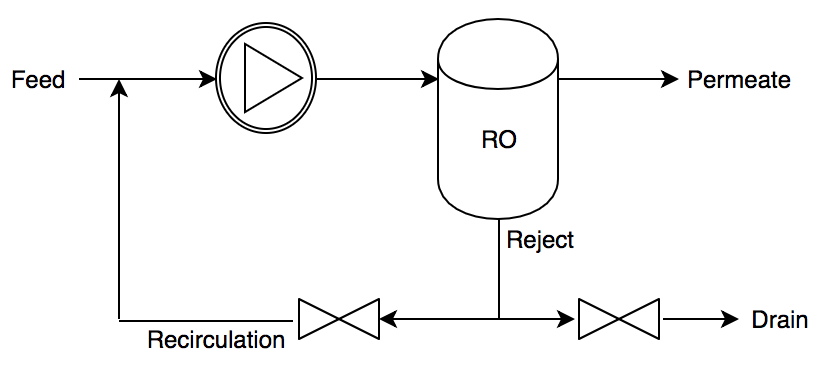
\includegraphics[width=0.5\textwidth]{Sys1}
    \caption{One pump system}
    \label{fig:System11}
\end{figure}
To obtain a system to investigate the membrane behaviour some different flowchart are considered. The current pump will be replaced by two pumps. Following requirements will be desirable when obtaining a updated model of the flowchart:
\begin{itemize}
\renewcommand\labelitemi{ }
\item Pressure drop over the membrane is high
\item Flow through membrane is high
\end{itemize}

\textbf{The model shall contribute with the following:}
\begin{itemize}
\renewcommand\labelitemi{ }
\item Permeate conductivity (minimised)
\item Fouling on the membrane (minimised)
\item Temperature dependencies 
\item Waste water going through drain (minimised)
\end{itemize}

\subsection{System 1}
Mainly two different systems containing two pumps were considered. The first system with one with pump on feed side and one pump on permeate side, as seen in Figure \ref{fig:FlowCInves1}. This setup contributes with the ability to create a net pressure over the membrane with a low, or even a under pressure on permeate side, whilst the feed pump creates a "high" pressure on feed side. Benefits with this implementation is the low energy consumption due to the ability to create negative pressure on permeate side. A high net driving pressure(pressure difference from feed to permeate side) can be achieved with rather low pressur on feed side. The withdrawal might be the implementation of the pump on permeate side. The water is used to feed dialysis machines and has high requirements on its purity. This sets high requirements on the pump, to not soil the purified water. 

\begin{figure}[h]
    \centering
    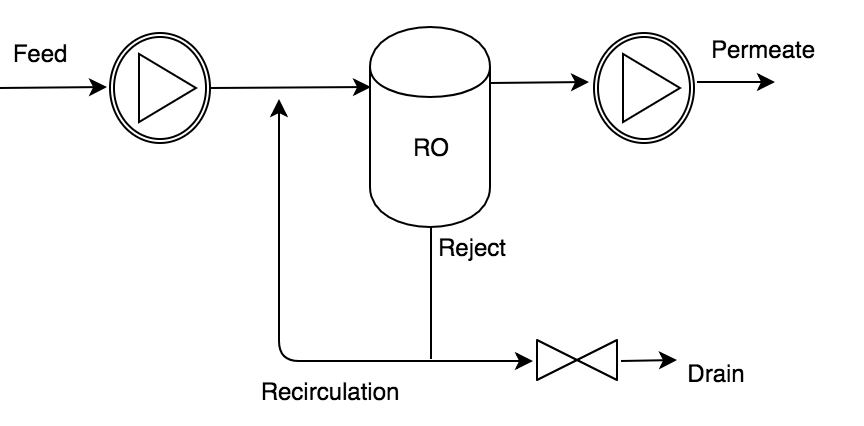
\includegraphics[width=0.4\textwidth]{FlowCInves1}
    \caption{System 1}
    \label{fig:FlowCInves1}
\end{figure}

\subsection{System 2}
The second system considered with one pump on feed side and one pump on reject side, in recirculation path, seen in Figure \ref{fig:Sys2}. The feed pump is used to create a high pressure on feed side and the pump in the recirculation path is used to control the flow in recirculation path. This contributes to control the recovery rate. Due to theory the membrane behaviour is dependent on feed and flow characteristics over the membrane, salt concentration and temperature. with this two pump solution the flow and pressure can be controlled independently and the membrane behaviour can be improved. The quality of the permeate water is ensured. \\
\\
\begin{figure}[h]
    \centering
    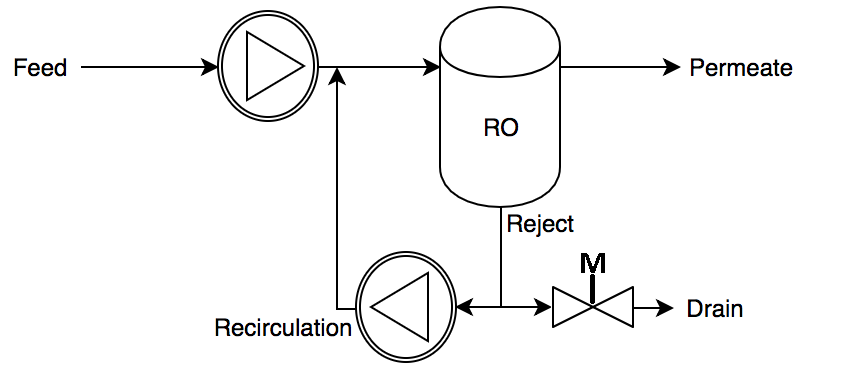
\includegraphics[width=0.4\textwidth]{Sys2}
    \caption{System 2}
    \label{fig:Sys2}
\end{figure}
\newpage

System 1 and System 2 contributes with the ability to control pressure and flow characteristics over the membrane. The big withdrawal with the implementation of a pump on permeate side is considered a high risk implementation and might put patients to high risks. System 1 is therefore precluded.

\section{Mapping}
In order to investigate the performance of the membrane pressure, flow, conductivity and temperature is  measured and logged. In the systems there are critical values of high pressure on feed side and reject side which makes it difficult to find measurement equipment that can handle both the high pressure and relatively low flows with no loss of pressure and required accuracy. \\
\\
Due to lack of instruments that could measure the flow under the high pressure some mapping of the flow from the pumps were done. The flow stream through the pumps were measured at different RPM and with different pressure resistance on the outlet. The flow is depending on the RPM with negligible difference depending on the applied outlet pressure from the pump. The mapped flow has an accuracy of $\pm$10\%.

\section{Implementation Test Rig}
\subsection{Current System}
In order to run all tests a physical rig was built. A first version to meet the specifications of the system used in the current water device were built according to Figure \ref{fig:MeasCurrSys}, with all the measurement sensors implemented. The rig contained, at the first stage: 1 pump with power supply, 1 RO-membrane, 3 needle valve, 1 drain valve, 1 water bath, three measurement sensors, pipes and couplings. The water bath is used to simulate different inlet water temperatures. The needle valves is used to adjust the pressure in the system to correspond with the real pressure characteristic in the water device. \\
\\
In order to log all signals and to run the system the Real-Time Target Machine described in Appendix A is connected with all significant signals. A GUI designed in Simulink to control the rig is connected to the rig. All control and feedback signals to and from the rig is handled in a built Simulink workspace where it is able to log and export all data to be able to analyse the system behaviour. All signals are filtered and displayed in real-time on a screen. \\
\\

\begin{figure}[h]
    \centering
    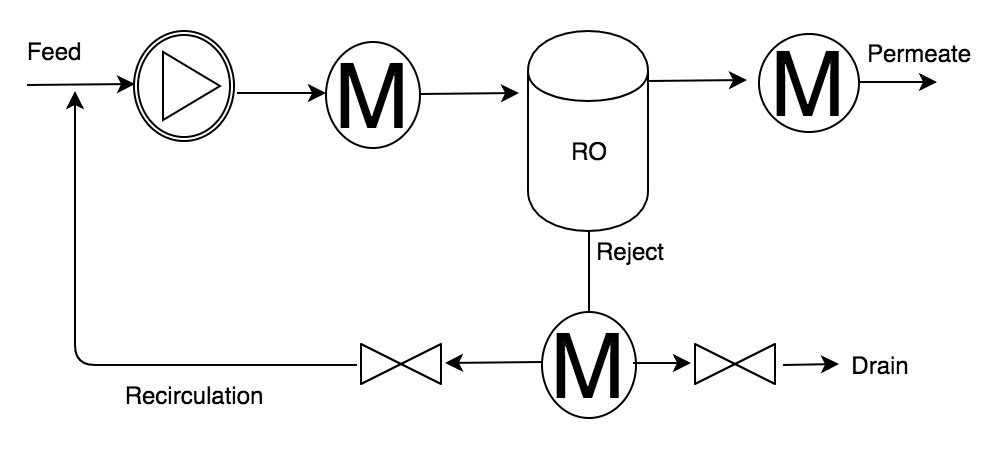
\includegraphics[width=0.4\textwidth]{MeasCurrSys}
    \caption{Current System, with measurement sensors}
    \label{fig:MeasCurrSys}
\end{figure}

\subsection{System 2  "Comparing system"}
The second system, System 2, were built by modifying the first rig, according to Figure \ref{fig:MeasSys2}. The second rig build contains: 2 pumps with power supply, 1 RO-membrane, 3 needle valve, 1 drain valve, 1 water bath, 1 flow meter, 3 measurement sensors, pipes and couplings. The water bath is used to simulate different inlet water temperatures. The needle valves is used to adjust the pressure in the system to correspond with the real pressure characteristic in the water device. The flow meter is used to measure the permeate flow from the membrane. \\
\\
The Simulink workspace, and the GUI was modified to be able to log all signal from the rig. All signals is displayed in real time as in the previous rig edition. Data is sampled and logged to be able to analyse the behaviour in the two pump system.  \\
\\
Different interfaces, as $i^{2}c$, Analog I/O, Digital inputs, PWM were used to implement the communication between the Real-Time Target Machine and measurement instruments. Circuits were built to transform voltage supply to required level for each component. All implementation of the communication and power supply can be seen in Figure \ref{fig:PressConn} - \ref{fig:PumpConn}. 

\begin{figure}[h]
    \centering
    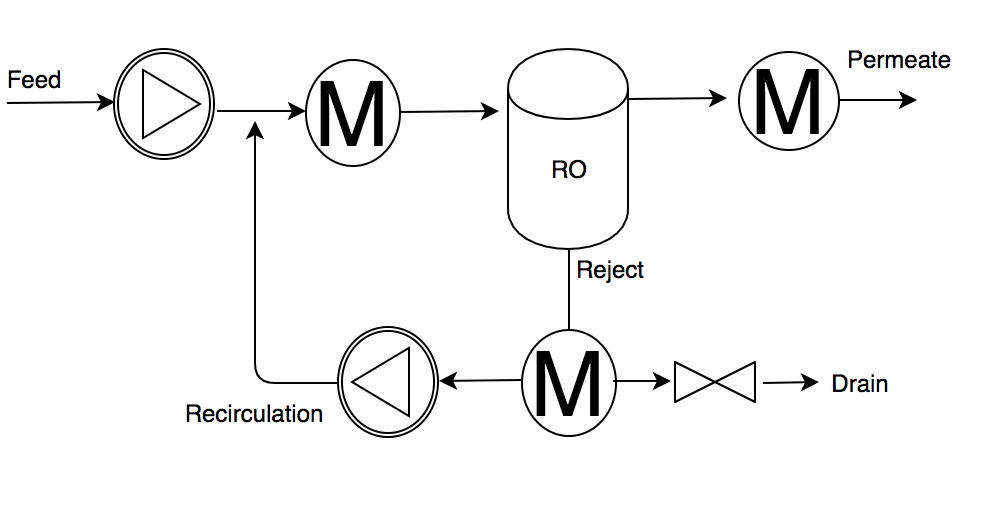
\includegraphics[width=0.4\textwidth]{MeasSys2}
    \caption{System 2, with measurement sensors}
    \label{fig:MeasSys2}
\end{figure}

\section{Test setup for membrane behaviour}
In order to compare results of the current system, furthermore called "Current System" and the updated system, System 2, some test will be done on the current setup. Reasonable values are investigated in order to meet requirements of the Water device. Corresponding points will be tested on the comparing system to evaluate any improvements on the membrane performance. The critical operational areas for the membrane is considered high temperatures (over 30 $^\circ$C) and high conductivity (over 2000 \SI{}{\micro\siemens}). The tests are performed in a range from 280-3000 \SI{}{\micro\siemens} and from 18-40 $^\circ$C. \\
\\
Points to be investigated can be seen in Table \ref{tab:testcases}. Same tests is performed on Current system and System 2 in order to analyse the difference in performance and membrane behaviour.\\
\begin{table}[h]
\begin{tabular}{|p{1.4cm}||p{2cm}|p{3.2cm}|p{1.8cm}|}
 \hline
 \textbf{Steady state }&Temperature&Feed Conductivity&Motor effect \\
 \hline
 1.1 & 18 $^\circ$C   & 280 \SI{}{\micro\siemens} & 60 \% \\
 1.2   &  18 $^\circ$C   & 500 \SI{}{\micro\siemens} & 60 \% \\
 1.3 &  18 $^\circ$C  &1000 \SI{}{\micro\siemens} & 60 \% \\
 1.4 &  18 $^\circ$C  &1000 \SI{}{\micro\siemens} & \textbf{80 \%} \\
 1.5 &18 $^\circ$C &2000 \SI{}{\micro\siemens}& 60 \%\\
 1.6 &18 $^\circ$C  &2000 \SI{}{\micro\siemens}& \textbf{80 \%}\\
 1.7   &18 $^\circ$C & 3000 \SI{}{\micro\siemens}&60 \% \\
 1.8   &18 $^\circ$C&3000 \SI{}{\micro\siemens}& \textbf{80 \%}\\
 \hline
 2.1 & 30 $^\circ$C & 280 \SI{}{\micro\siemens}&60 \%\\
 2.2 & 30 $^\circ$C &500 \SI{}{\micro\siemens}& 60 \%\\
 2.3 & 30 $^\circ$C&1000 \SI{}{\micro\siemens}& 60 \%\\
 2.4 & 30 $^\circ$C&1000 \SI{}{\micro\siemens}& \textbf{80 \%}\\
 2.5 & 30 $^\circ$C&2000 \SI{}{\micro\siemens}& 60 \%\\
 2.6 & 30 $^\circ$C&2000 \SI{}{\micro\siemens}& \textbf{80 \%}\\
 2.7 & 30 $^\circ$C& 3000 \SI{}{\micro\siemens}&60 \%\\
 2.8 & 30 $^\circ$C& 3000 \SI{}{\micro\siemens}&\textbf{80 \%}\\
 \hline 
 3.1 & 40 $^\circ$C& 280 \SI{}{\micro\siemens}& 60 \%\\
 3.2 & 40 $^\circ$C &500 \SI{}{\micro\siemens}& 60 \%\\
 3.3 & 40 $^\circ$C  & 1000 \SI{}{\micro\siemens}& 60 \%\\
 3.4 & 40 $^\circ$C  & 1000 \SI{}{\micro\siemens}& \textbf{80 \%}\\
 3.5 & 40 $^\circ$C&2000 \SI{}{\micro\siemens}& 60 \%\\
 3.6 & 40 $^\circ$C &2000 \SI{}{\micro\siemens}& \textbf{80 \%}\\
 3.7 & 40$^\circ$C &3000 \SI{}{\micro\siemens}& 60 \%\\
 3.8 & 40$^\circ$C &3000 \SI{}{\micro\siemens}& \textbf{80 \%}\\
\hline
\end{tabular}
\caption{Testcases}
    \label{tab:testcases} 
\end{table}


\newpage


\section{Design of control algorithms}

Investigating tests on System 2, Figure \ref{fig:Sys2}, were executed prior the design of the control algorithms to receive required reference signals to the pumps and drain valve. During the tests one parameter at a time changed while the others were kept constant. In test 1, seen in Figure \ref{fig:PreTestReg1} the pump in recycle path were the changing parameter and in Test 2, seen in Figure \ref{fig:PreTestReg3} the pressurising pump on inlet side were the changing parameter. 










\chapter{Results}
% !TEX root = /Users/Gela/Desktop/Thesis_latex/thesis.tex
\section{Modeling}
A physical model of the membrane were made and the given results can be seen below. In figure \ref{fig:simscape} the flowchart is given. The RO-membrane is simulated with three nodes; feed, product and reject, and an extra input temp. The temp node gives freedom to simulate the behaviour of the membrane in different temperature ranges. The model consists the pump, pipes, valves and tank. The water in the tank can be set to contain any salt koncentration to be able to simulate different conductivity values. The speed of the pumps can be changed to change the flow and pressure characteristic over the membrane in the model.\\
\\
\begin{figure}[h]
\label{fig:simscape}
\centering
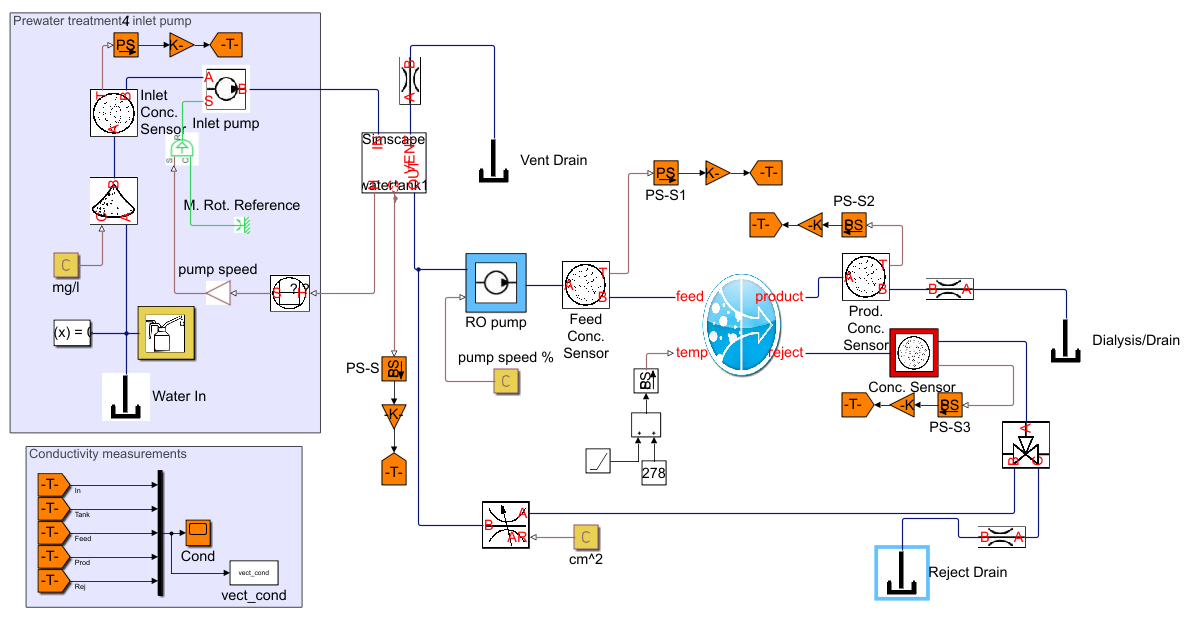
\includegraphics[width=\textwidth]{simscape_fc1.PNG}
\caption{Model made in Matlab tool Simscape}
\end{figure}


\subsection{Temperature}
In figure \ref{fig:temp} the simulated temperature, 278-316 K is shown. All plots \ref{fig:msaltf} - \ref{fig:conden} shows the behaviour over a simulated time of 2000 s and a temperature range of 278-316 K. Pump speed is kept constant. The temperature correction factor, TCF, in figure \ref{fig:tcf} is the temperature dependent parameter implemented in the simulated model to receive the differences of the behaviour of the membrane. At 298 K TCF is equal to 1. Below and above it is adjusted to compensate for the differences of the membrane behaviour. \\
\\
\begin{figure}[h]
  \centering
  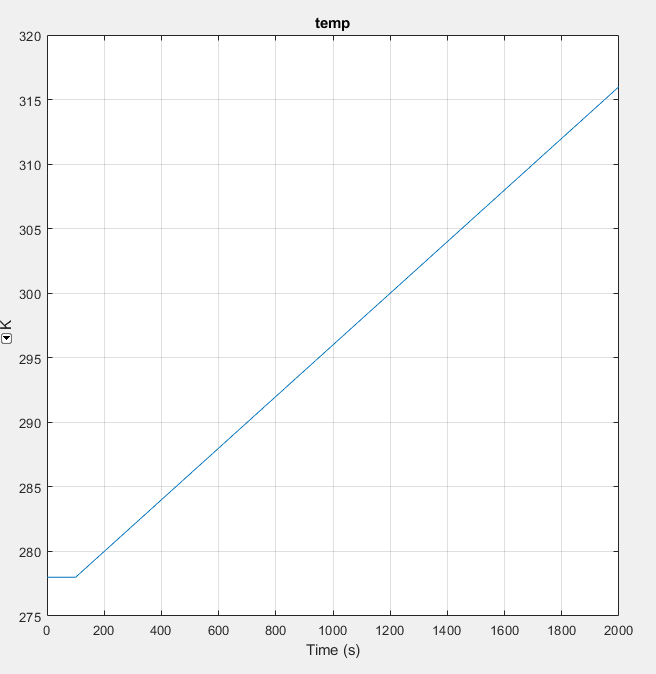
\includegraphics[width=0.5\linewidth]{temp.PNG}
  \caption{Temperature}
  \label{fig:temp}
\end{figure}
\begin{figure}[h]
\centering
    \centering
    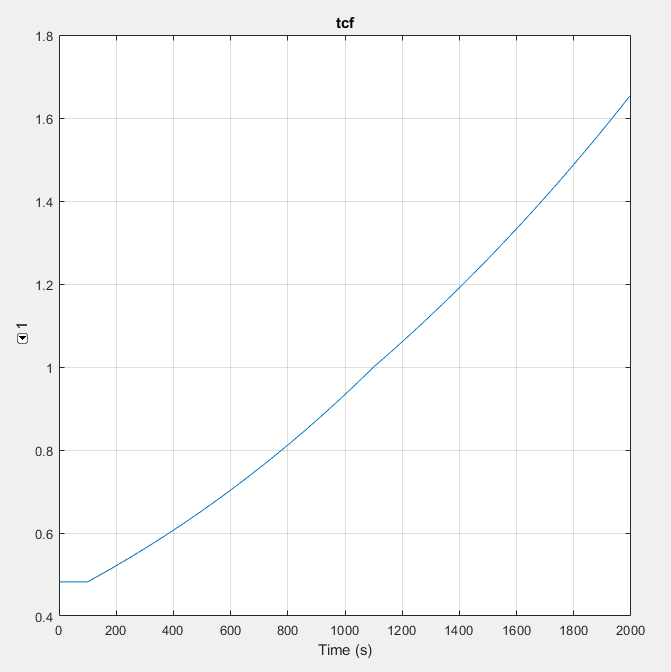
\includegraphics[width=0.5\textwidth]{tcf.PNG}
    \caption{Temperature correction factor}
    \label{fig:tcf}
\end{figure}

\subsection{Salt koncentration}

In figure \ref{fig:msaltf} the salt koncentration in kg/s on feed side of the membrane is shown. The concentration increases over the simulated time and change in temperature. \\
In figure \ref{fig:msaltp} the salt koncentration on product side is shown. Due to the mass balance equation in XXXX the sign is negative, and the koncentration increases with temperature.\\
In figure \ref{fig:msaltr} the salt koncentration on reject side is shown. It increases a little with temperature (negative sign due to the mass balance equations).\\
The product salt koncentration increases with from a value of  0.8 - 0.96 kg/s. The product water koncentration increases from (-) 0.2 - 1.8 kg/s. The reject salt koncentration increases from (-) 0.8 - 0.96 kg/s.\\
\\
\begin{figure}[h]
\centering
    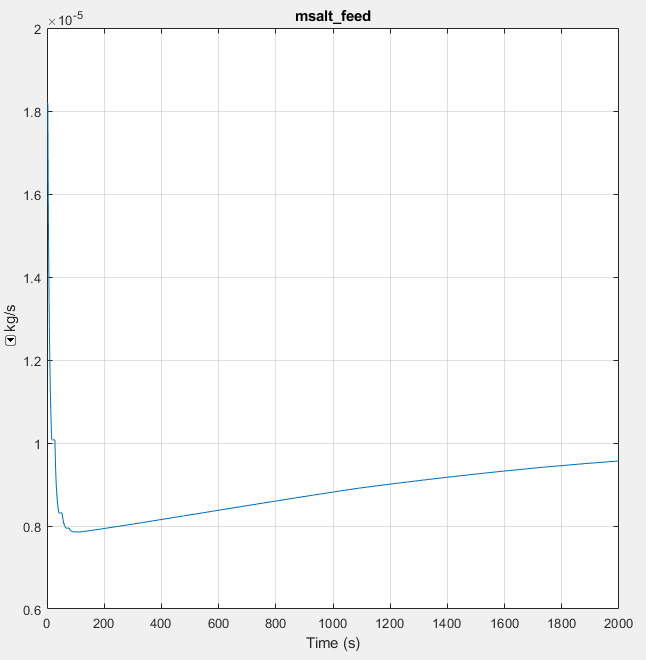
\includegraphics[width=0.5\textwidth]{msalt_feed.PNG}
    \caption{Salt concentration feedwater}
    \label{fig:msaltf}
\end{figure}
\begin{figure}[h]
\centering
  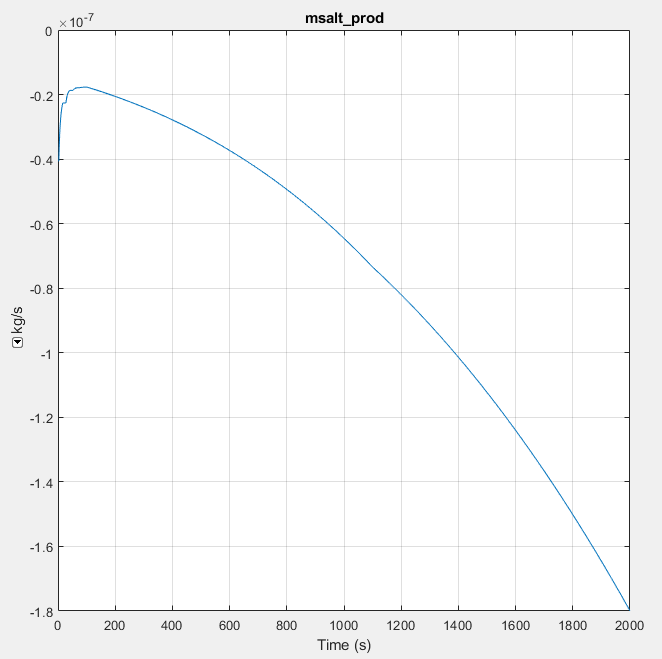
\includegraphics[width=0.5\linewidth]{msalt_prod.PNG}
  \caption{Salt concentration productwater}
  \label{fig:msaltp}
\end{figure}
\begin{figure}[h]
  \centering
  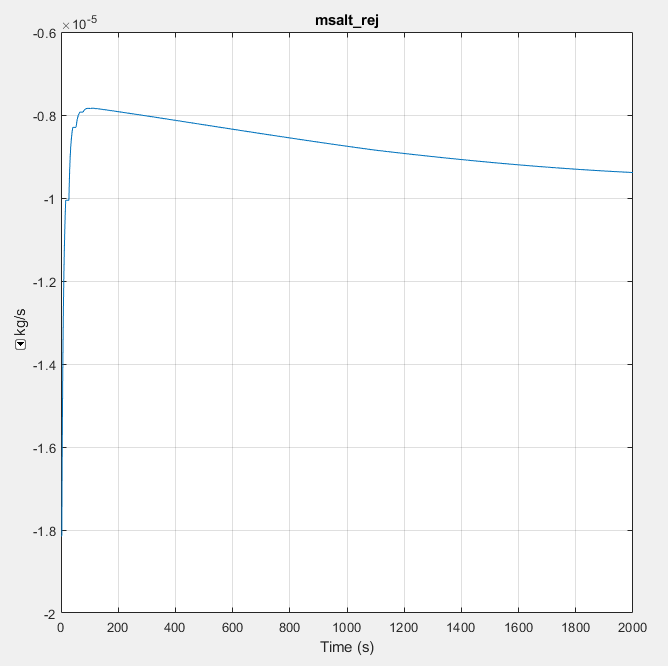
\includegraphics[width=0.5\linewidth]{msalt_rej.PNG}
  \caption{Salt concentration reject water}
  \label{fig:msaltr}
\end{figure}
Figure \ref{fig:qf} - \ref{fig:qrej} shows the flow in the three nodes; feed, product and reject. The mass balance equation in XXXX gives negative sign on reject and product side. The feed water flow increases negligible from 8.441-8.444 l/min. Product water flow increases from (-) 0.62-1.42 l/min. Reject water flow decreases from (-) 7.82-7.2 l/min. \\
\\

\subsection{Flow}
\begin{figure}[h]
  \centering
  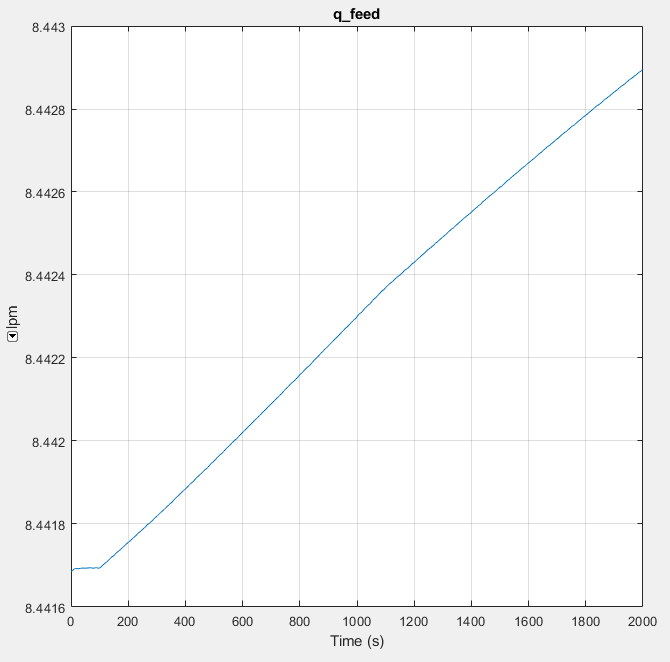
\includegraphics[width=0.5\linewidth]{q_feed.PNG}
  \caption{Flow feed side}
  \label{fig:qf}
\end{figure}
\begin{figure}[h]
  \centering
  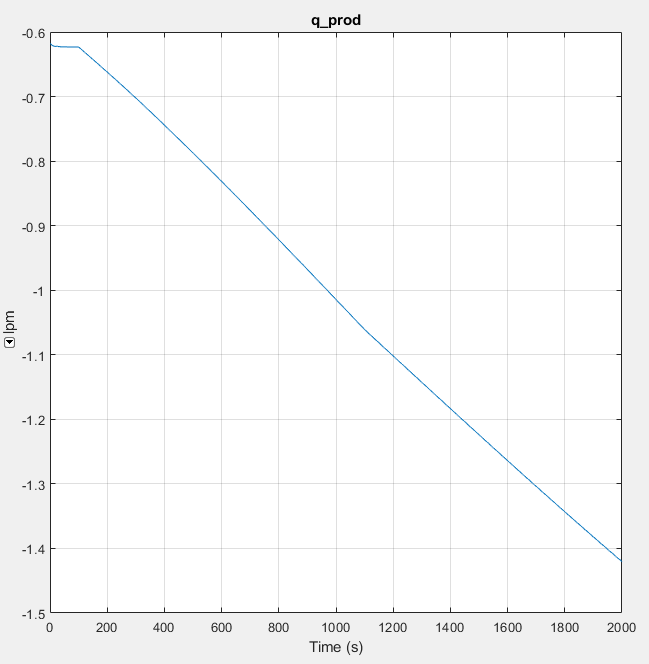
\includegraphics[width=0.5\linewidth]{q_prod.PNG}
  \caption{Flow product side}
  \label{fig:qp}
\end{figure}
\begin{figure}[h]
  \centering
  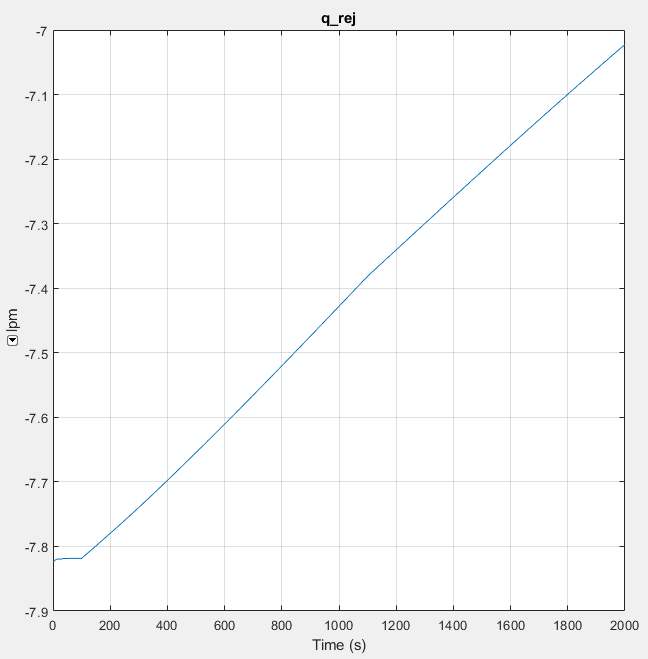
\includegraphics[width=0.5\linewidth]{q_rej.PNG}
  \caption{Flow reject side}
  \label{fig:qrej}
\end{figure}

\subsection{Pressure}
Figure \ref{fig:deltap} shows pressure difference from feed side to product side. The pressure decreases from (-) 11.5-7.7 bar when temperature changes from 278-316 K. \\
\\
\begin{figure}[h]
  \centering
  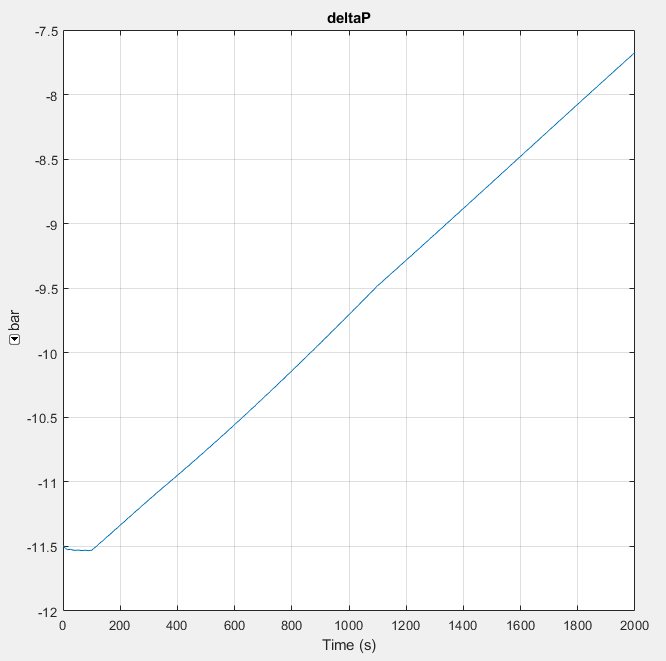
\includegraphics[width=0.5\linewidth]{deltap.PNG}
  \caption{Pressure drop feed side to product side}
  \label{fig:deltap}
\end{figure}

\subsection{Conductivity}
Figure \ref{fig:conden} displays the conductivity in feed, product and reject side. The conductivity in all nodes increases when temperature increases.\\
\\
\begin{figure}[h]
  \label{fig:conden}
  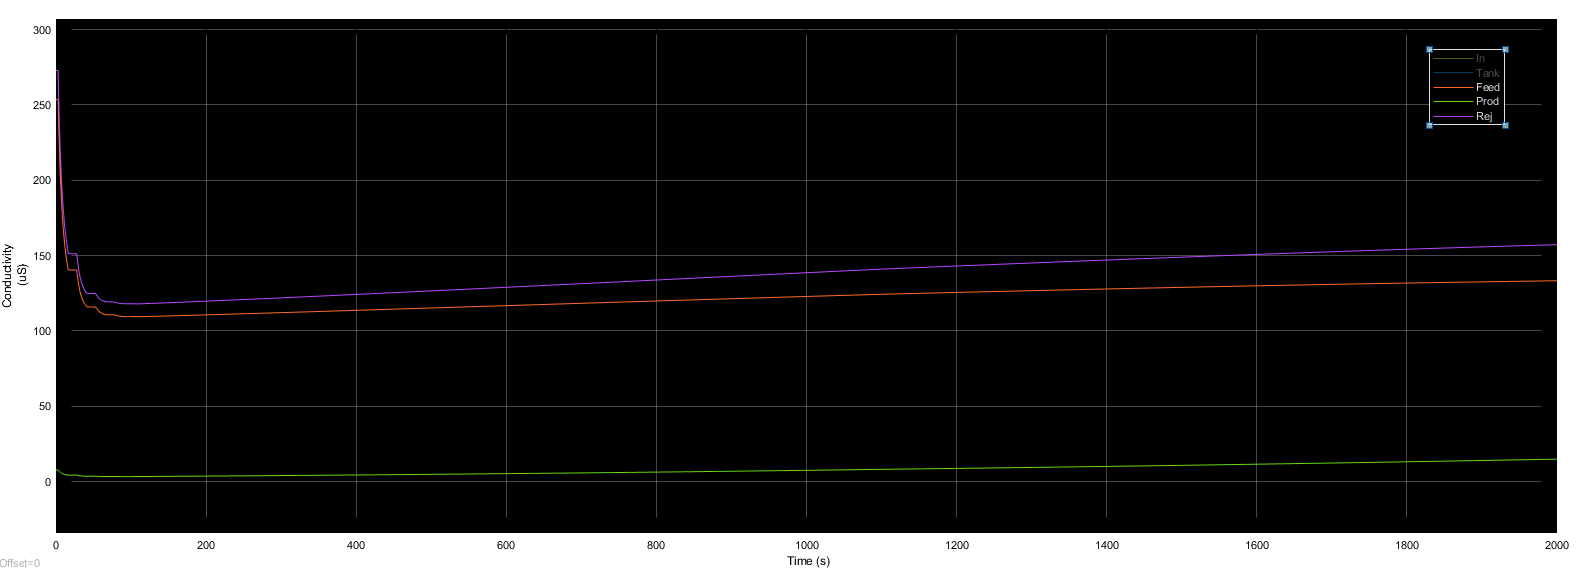
\includegraphics[width=1.1\linewidth]{cond.PNG}
  \caption{Conductivity in feed, reject and product side}
\end{figure}

\newpage


\section{Flowchart investigation}
By changing the flow path in the test setup both the one pump system and two pump system could be investigated and their performance could be compared. Both Systems were considered fulfilling most of the requirements, section \ref{framing}, for an updated version. \\

One pump system, figure \ref{fig:FlowCInves1}, The one pump system was designed to use both a tank and the recirculation loop as a water source and to create pressure by generating a large flow over the membrane and recirculation restrictor. \\


Two pump system, figure \ref{fig:Sys2}, In the two pump system the water path was modified so that the feed pump only used a tank as a source and pressureized the entire recirculation loop. The recirculation pump was used to recirculate the already\\ pressureized water within the recirculation loop.\\


An overview of the systems can be seen below.\\
\begin{figure}[h]
\centering
\begin{minipage}{.5\textwidth}
    \centering
    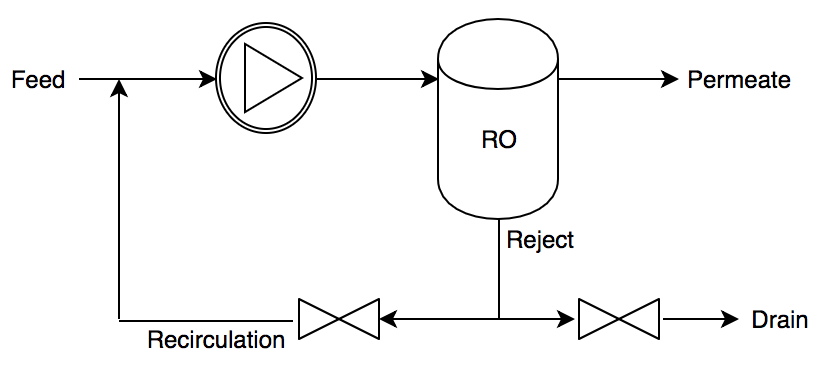
\includegraphics[width=0.8\textwidth]{Sys1}
    \caption{One pump system}
    \label{fig:System1}
\end{minipage}%
\begin{minipage}{.5\textwidth}
  \centering
  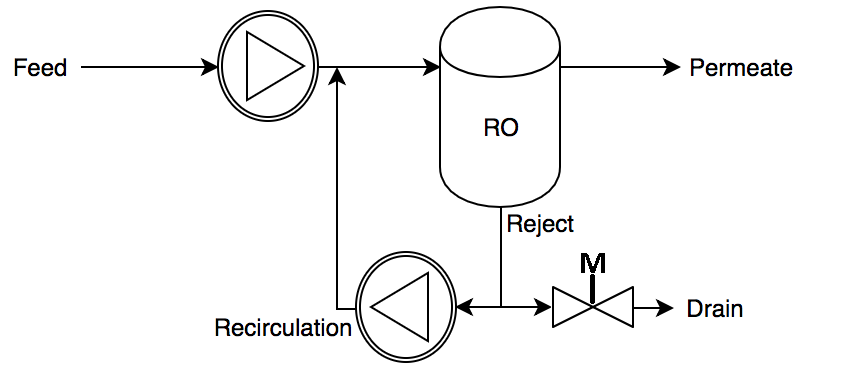
\includegraphics[width=.8\linewidth]{Sys2}
  \caption{Two pump system}
  \label{fig:System2}
\end{minipage}
\end{figure}

\newpage

\section{Implementation Test Rig}


\subsection{Connections}
In Figure (\ref{fig:PressConn}-\ref{fig:PumpConn}) all connections in the test rig is displayed. The whole rig can be seen in \ref{fig:Rig1} and \ref{fig:Rig2}

\begin{figure}[h]
    \centering
    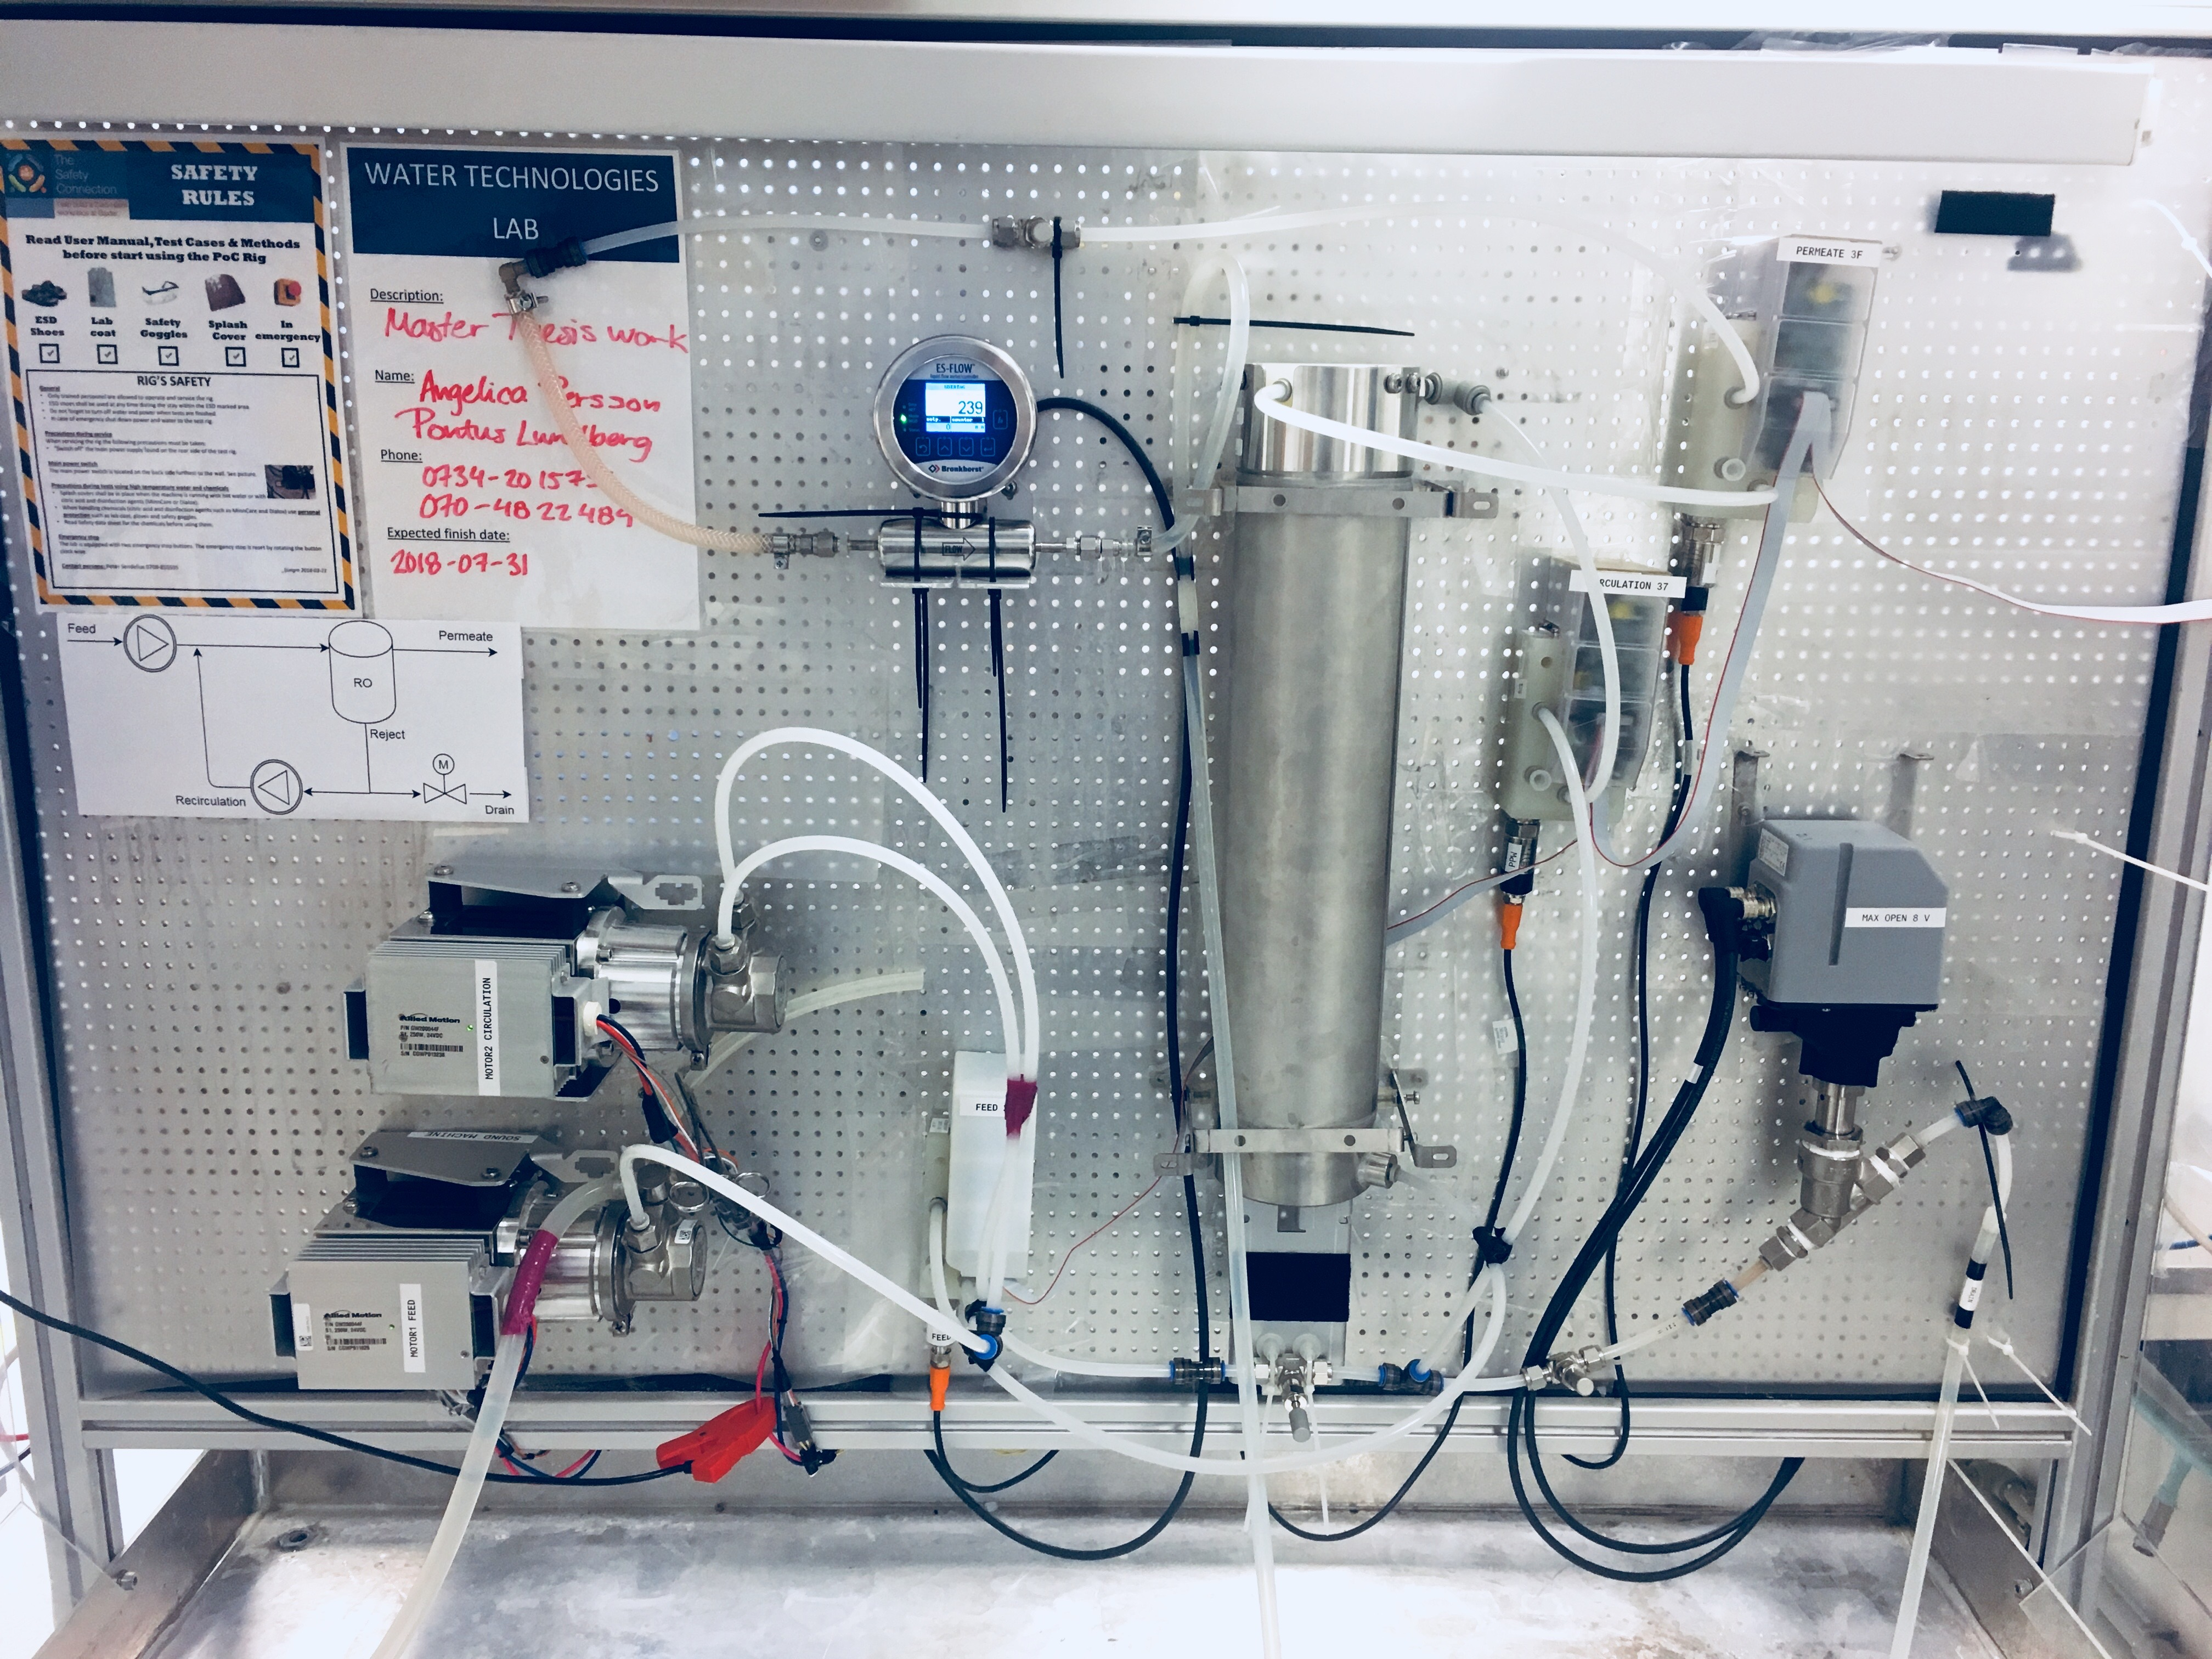
\includegraphics[width=0.5\textwidth]{Rig1}
    \caption{The rig built at Baxter Lund AB, with RO-membrane, pumps, pipes, flowmeter, measuremet sensors and valves}
    \label{fig:Rig1}
\end{figure}

\begin{figure}[h]
    \centering
    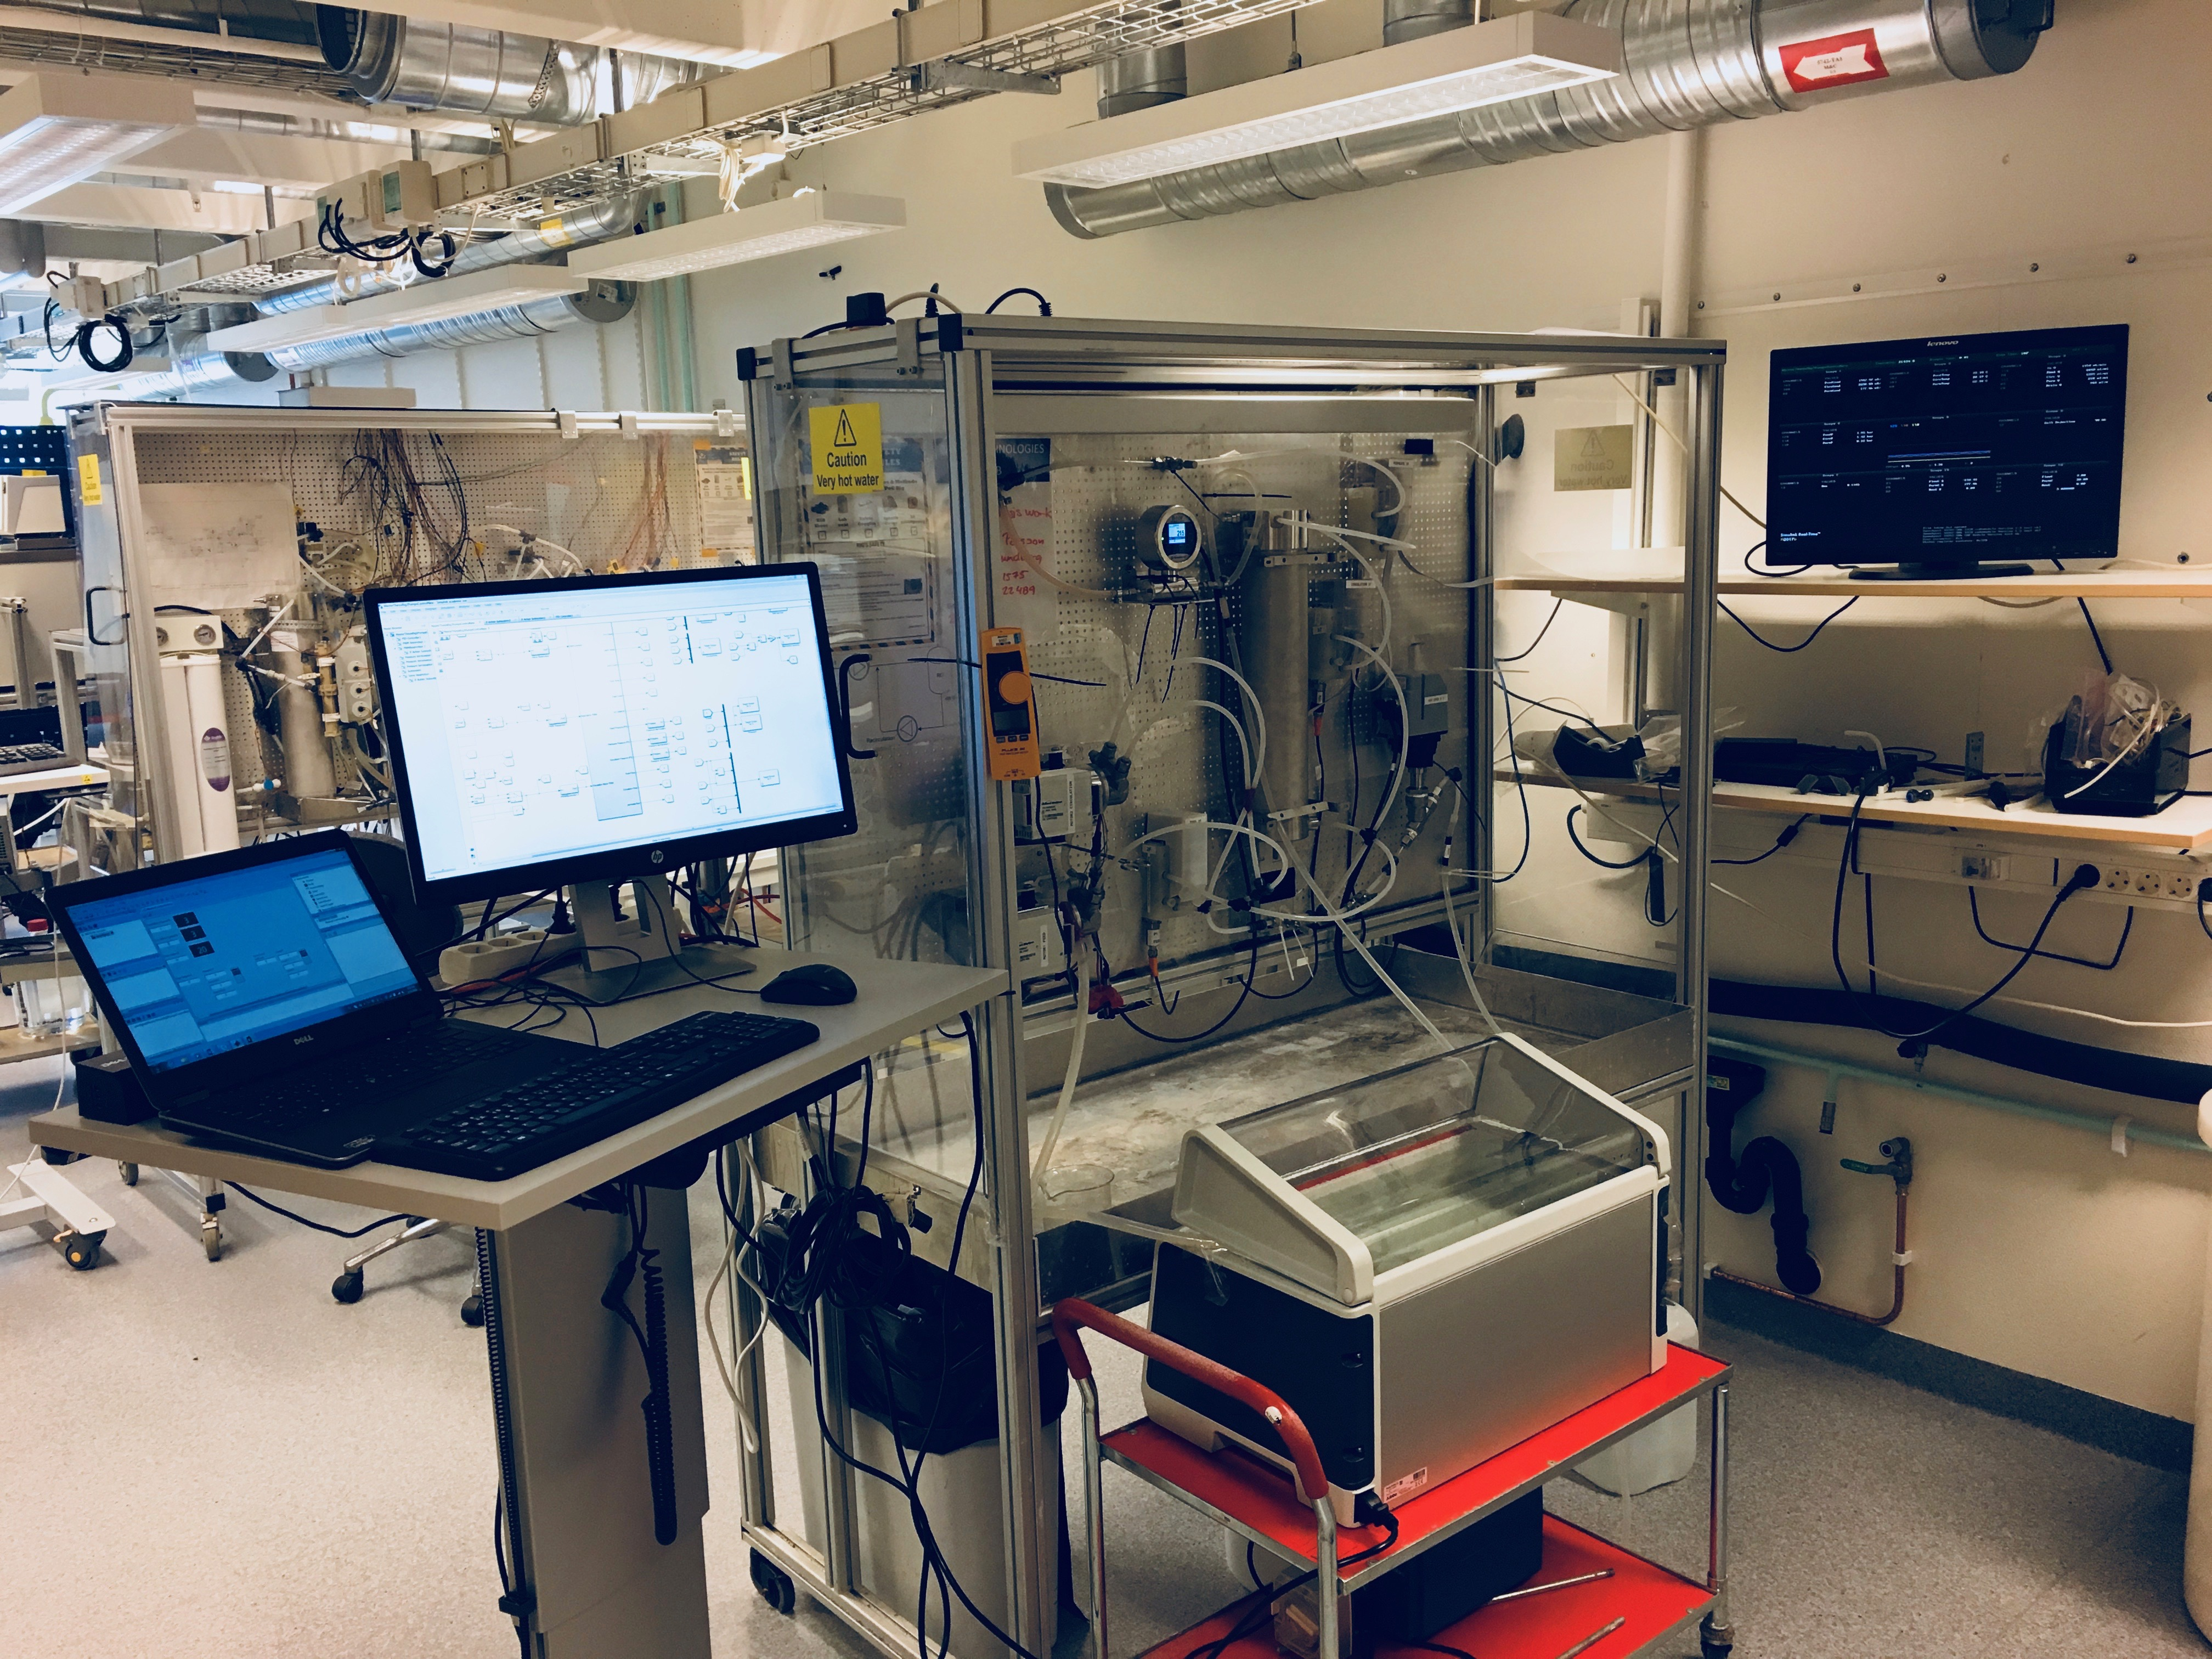
\includegraphics[width=0.5\textwidth]{Rig2}
    \caption{The full setup built at Baxter Lund AB, with simulink implementation, GUI, display and water bath}
    \label{fig:Rig2}
\end{figure}


\begin{figure}[h]
    \centering
    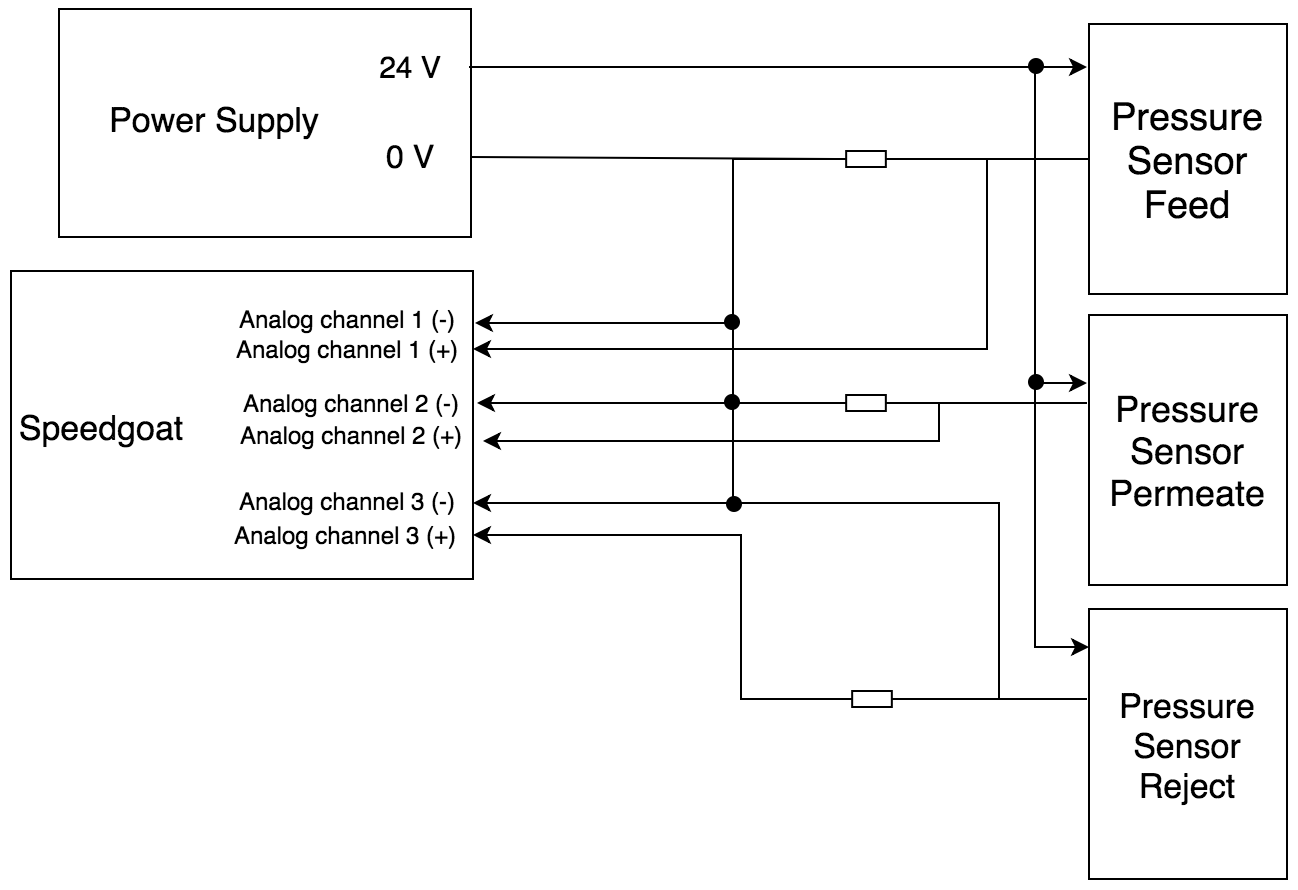
\includegraphics[width=0.6\textwidth]{PressConn}
    \caption{Connections Pressure sensors}
    \label{fig:PressConn}
\end{figure}

\newpage

\begin{figure}[h]
    \centering
    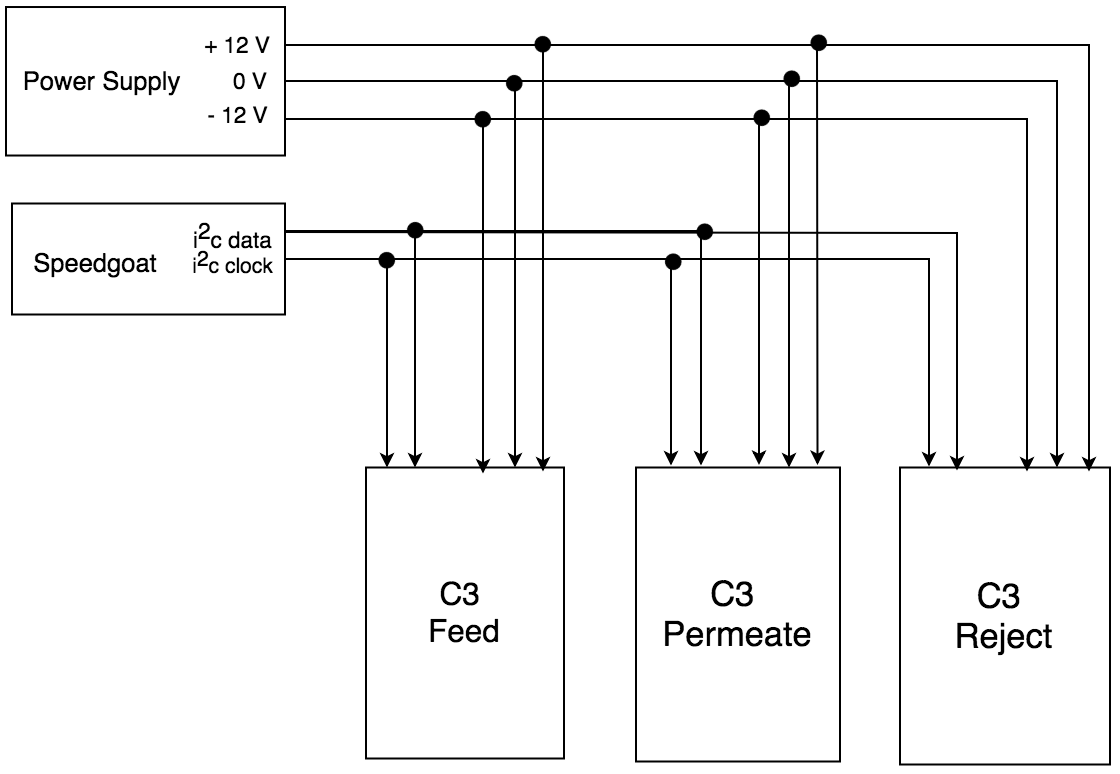
\includegraphics[width=0.6\textwidth]{C3Conn}
    \caption{Connections measurement blocks, C3}
    \label{fig:C3Conn}
\end{figure}

\begin{figure}[h]
    \centering
    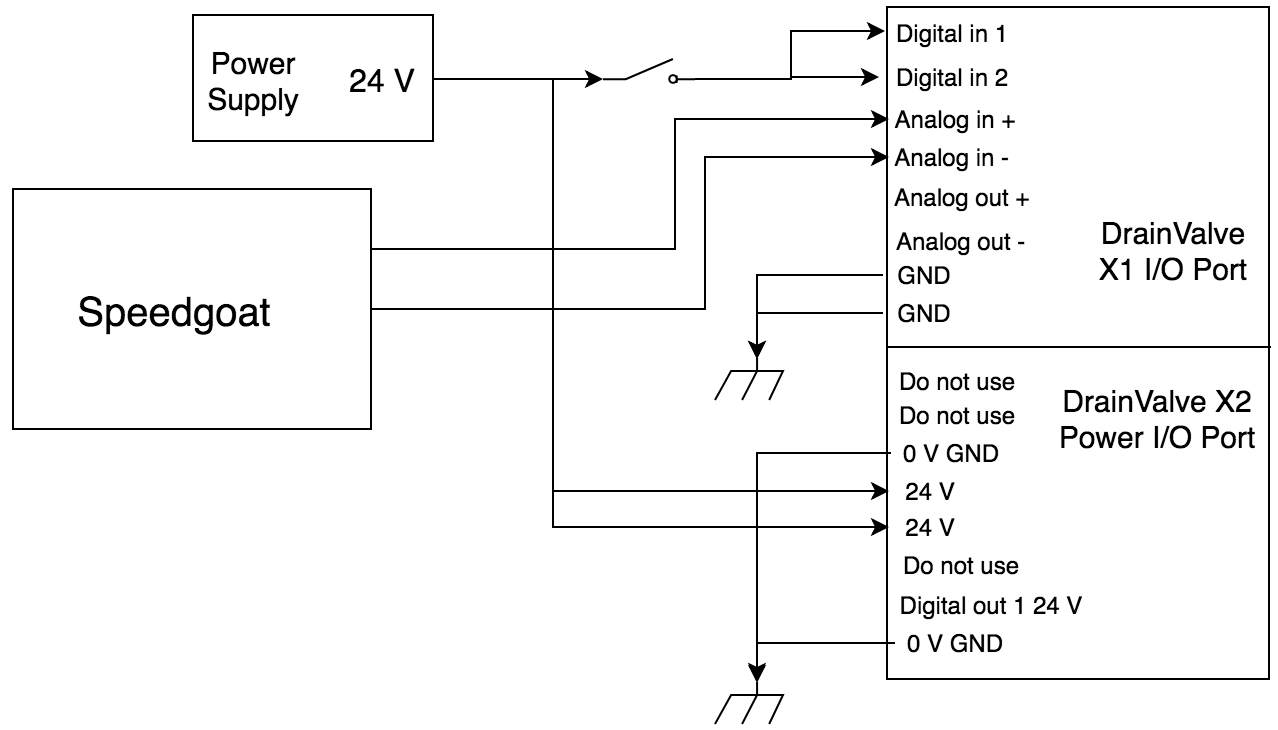
\includegraphics[width=0.6\textwidth]{ValveConn}
    \caption{Connections Drain Valve}
    \label{fig:ValveConn}
\end{figure}

\newpage

\begin{figure}[H]
    \centering
    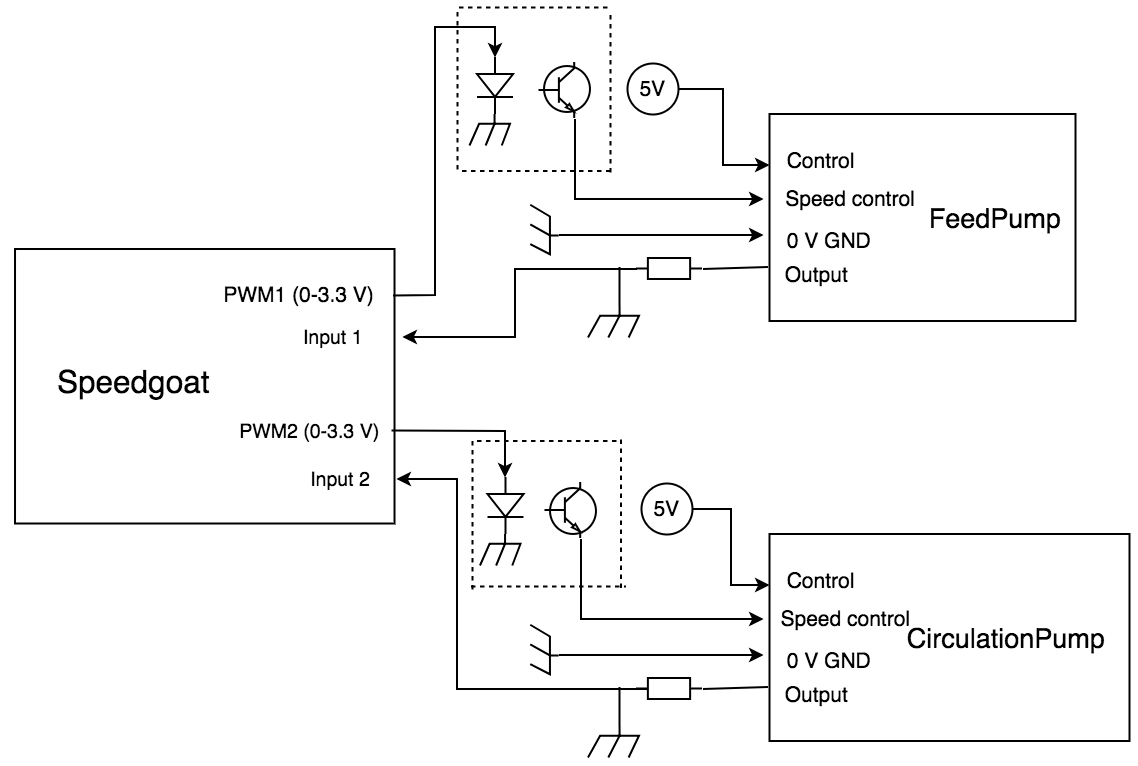
\includegraphics[width=0.6\textwidth]{PumpConn}
    \caption{Connections pumps}
    \label{fig:PumpConn}
\end{figure}
\begin{figure}[H]
    \centering
    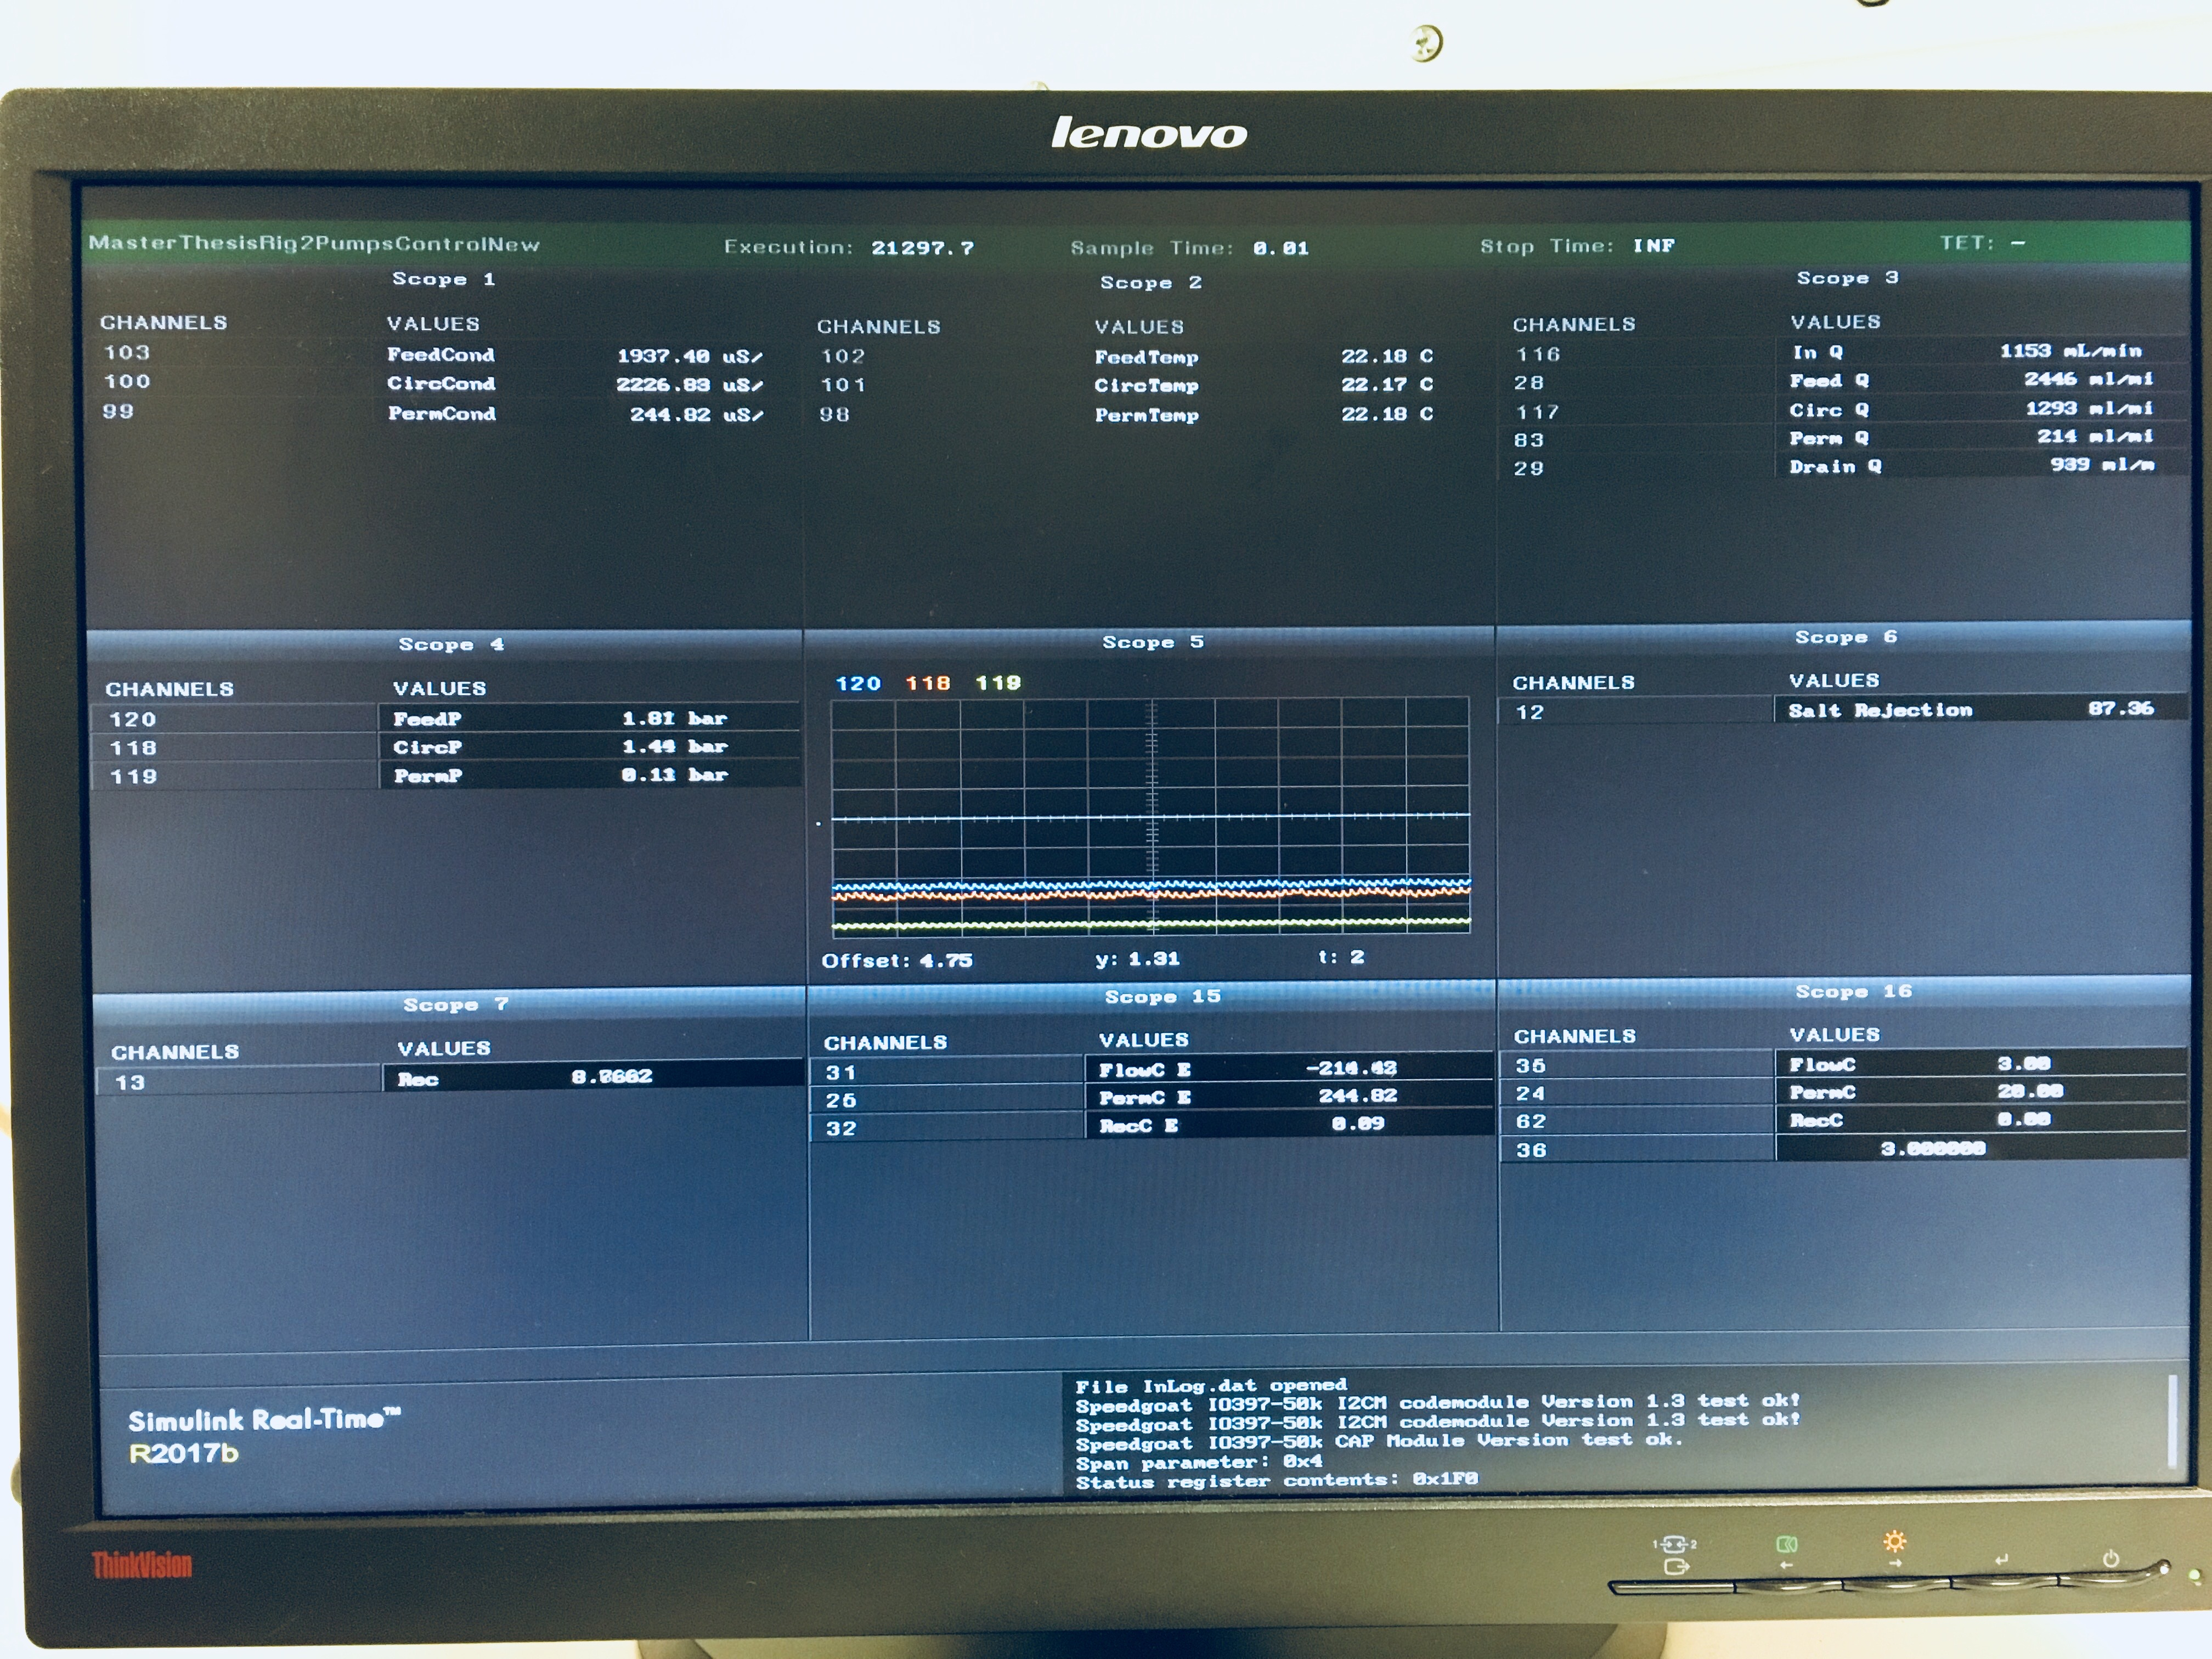
\includegraphics[width=0.6\textwidth]{Display}
    \caption{The Display with all key values, read from sensors in the rig}
    \label{fig:display}
\end{figure}
\begin{figure}[H]
    \centering
    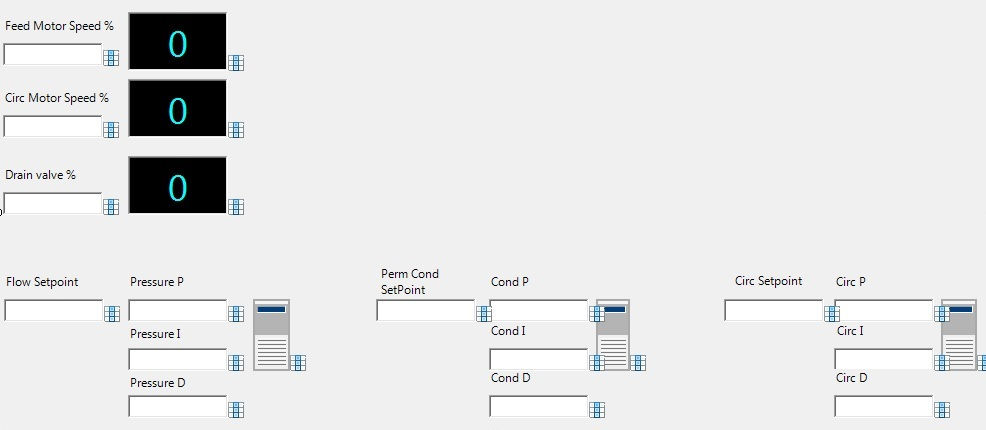
\includegraphics[width=0.6\textwidth]{GUI}
    \caption{The GUI implemented in Simulink and used to control the rig}
    \label{fig:gui}
\end{figure}


\newpage


\section{Investigation on membrane behaviour}

In order to compare the two systems and understand how the membrane performed in different working conditions both systems needed to be tested. The tests were conducted by controlling the temperature, pumps and the conductivity in the recirculation loop and log how the different conditions affected the system and the membrane. 

The tests were conducted by changing the temperature, recirculation conductivity and pump speed and meassure how the system behaved once it had reached steady state. The tests were divided into three test sequences. One test sequence was performed with room temperatured water (19 C), one with water heated to 30 C and in the last test sequence the water was heated to 40 C. Every test sequence included data from 8 steady state points with different settings on feed conductivity and pump speed. The test sequences are displayed in the table below. 

\begin{table}[h]
\centering
\begin{tabular}{|p{1.4cm}||p{2cm}|p{3.2cm}|p{1.8cm}|}
 \hline
 \textbf{Steady state }&Temperature&Feed Conductivity&Motor effect \\
 \hline
 1.1 & 18 $^\circ$C   & 280 \SI{}{\micro\siemens} & 60 \% \\
 1.2   &  18 $^\circ$C   & 500 \SI{}{\micro\siemens} & 60 \% \\
 1.3 &  18 $^\circ$C  &1000 \SI{}{\micro\siemens} & 60 \% \\
 1.4 &  18 $^\circ$C  &1000 \SI{}{\micro\siemens} & \textbf{80 \%} \\
 1.5 &18 $^\circ$C &2000 \SI{}{\micro\siemens}& 60 \%\\
 1.6 &18 $^\circ$C  &2000 \SI{}{\micro\siemens}& \textbf{80 \%}\\
 1.7   &18 $^\circ$C & 3000 \SI{}{\micro\siemens}&60 \% \\
 1.8   &18 $^\circ$C&3000 \SI{}{\micro\siemens}& \textbf{80 \%}\\
 \hline
 2.1 & 30 $^\circ$C & 280 \SI{}{\micro\siemens}&60 \%\\
 2.2 & 30 $^\circ$C &500 \SI{}{\micro\siemens}& 60 \%\\
 2.3 & 30 $^\circ$C&1000 \SI{}{\micro\siemens}& 60 \%\\
 2.4 & 30 $^\circ$C&1000 \SI{}{\micro\siemens}& \textbf{80 \%}\\
 2.5 & 30 $^\circ$C&2000 \SI{}{\micro\siemens}& 60 \%\\
 2.6 & 30 $^\circ$C&2000 \SI{}{\micro\siemens}& \textbf{80 \%}\\
 2.7 & 30 $^\circ$C& 3000 \SI{}{\micro\siemens}&60 \%\\
 2.8 & 30 $^\circ$C& 3000 \SI{}{\micro\siemens}&\textbf{80 \%}\\
 \hline 
 3.1 & 40 $^\circ$C& 280 \SI{}{\micro\siemens}& 60 \%\\
 3.2 & 40 $^\circ$C &500 \SI{}{\micro\siemens}& 60 \%\\
 3.3 & 40 $^\circ$C  & 1000 \SI{}{\micro\siemens}& 60 \%\\
 3.4 & 40 $^\circ$C  & 1000 \SI{}{\micro\siemens}& \textbf{80 \%}\\
 3.5 & 40 $^\circ$C&2000 \SI{}{\micro\siemens}& 60 \%\\
 3.6 & 40 $^\circ$C &2000 \SI{}{\micro\siemens}& \textbf{80 \%}\\
 3.7 & 40$^\circ$C &3000 \SI{}{\micro\siemens}& 60 \%\\
 3.8 & 40$^\circ$C &3000 \SI{}{\micro\siemens}& \textbf{80 \%}\\
\hline
\end{tabular}
\caption{Testcases}
    \label{tab:test cases} 
\end{table}


\newpage
\subsection{Current system, Test sequence 1, part 1}

The water in the tank was heated while the test was running. Because of this, the test was split up in two parts, first the motor was set to 60\% and steady state 1.1, 1.2, 1.3, 1.5 and 1.7 were investigated. In the part 2, the motor was set to 80 \% and steady state 1.4, 1.6 and 1.8 were investigated. 

\begin{figure}[h]
    \centering
    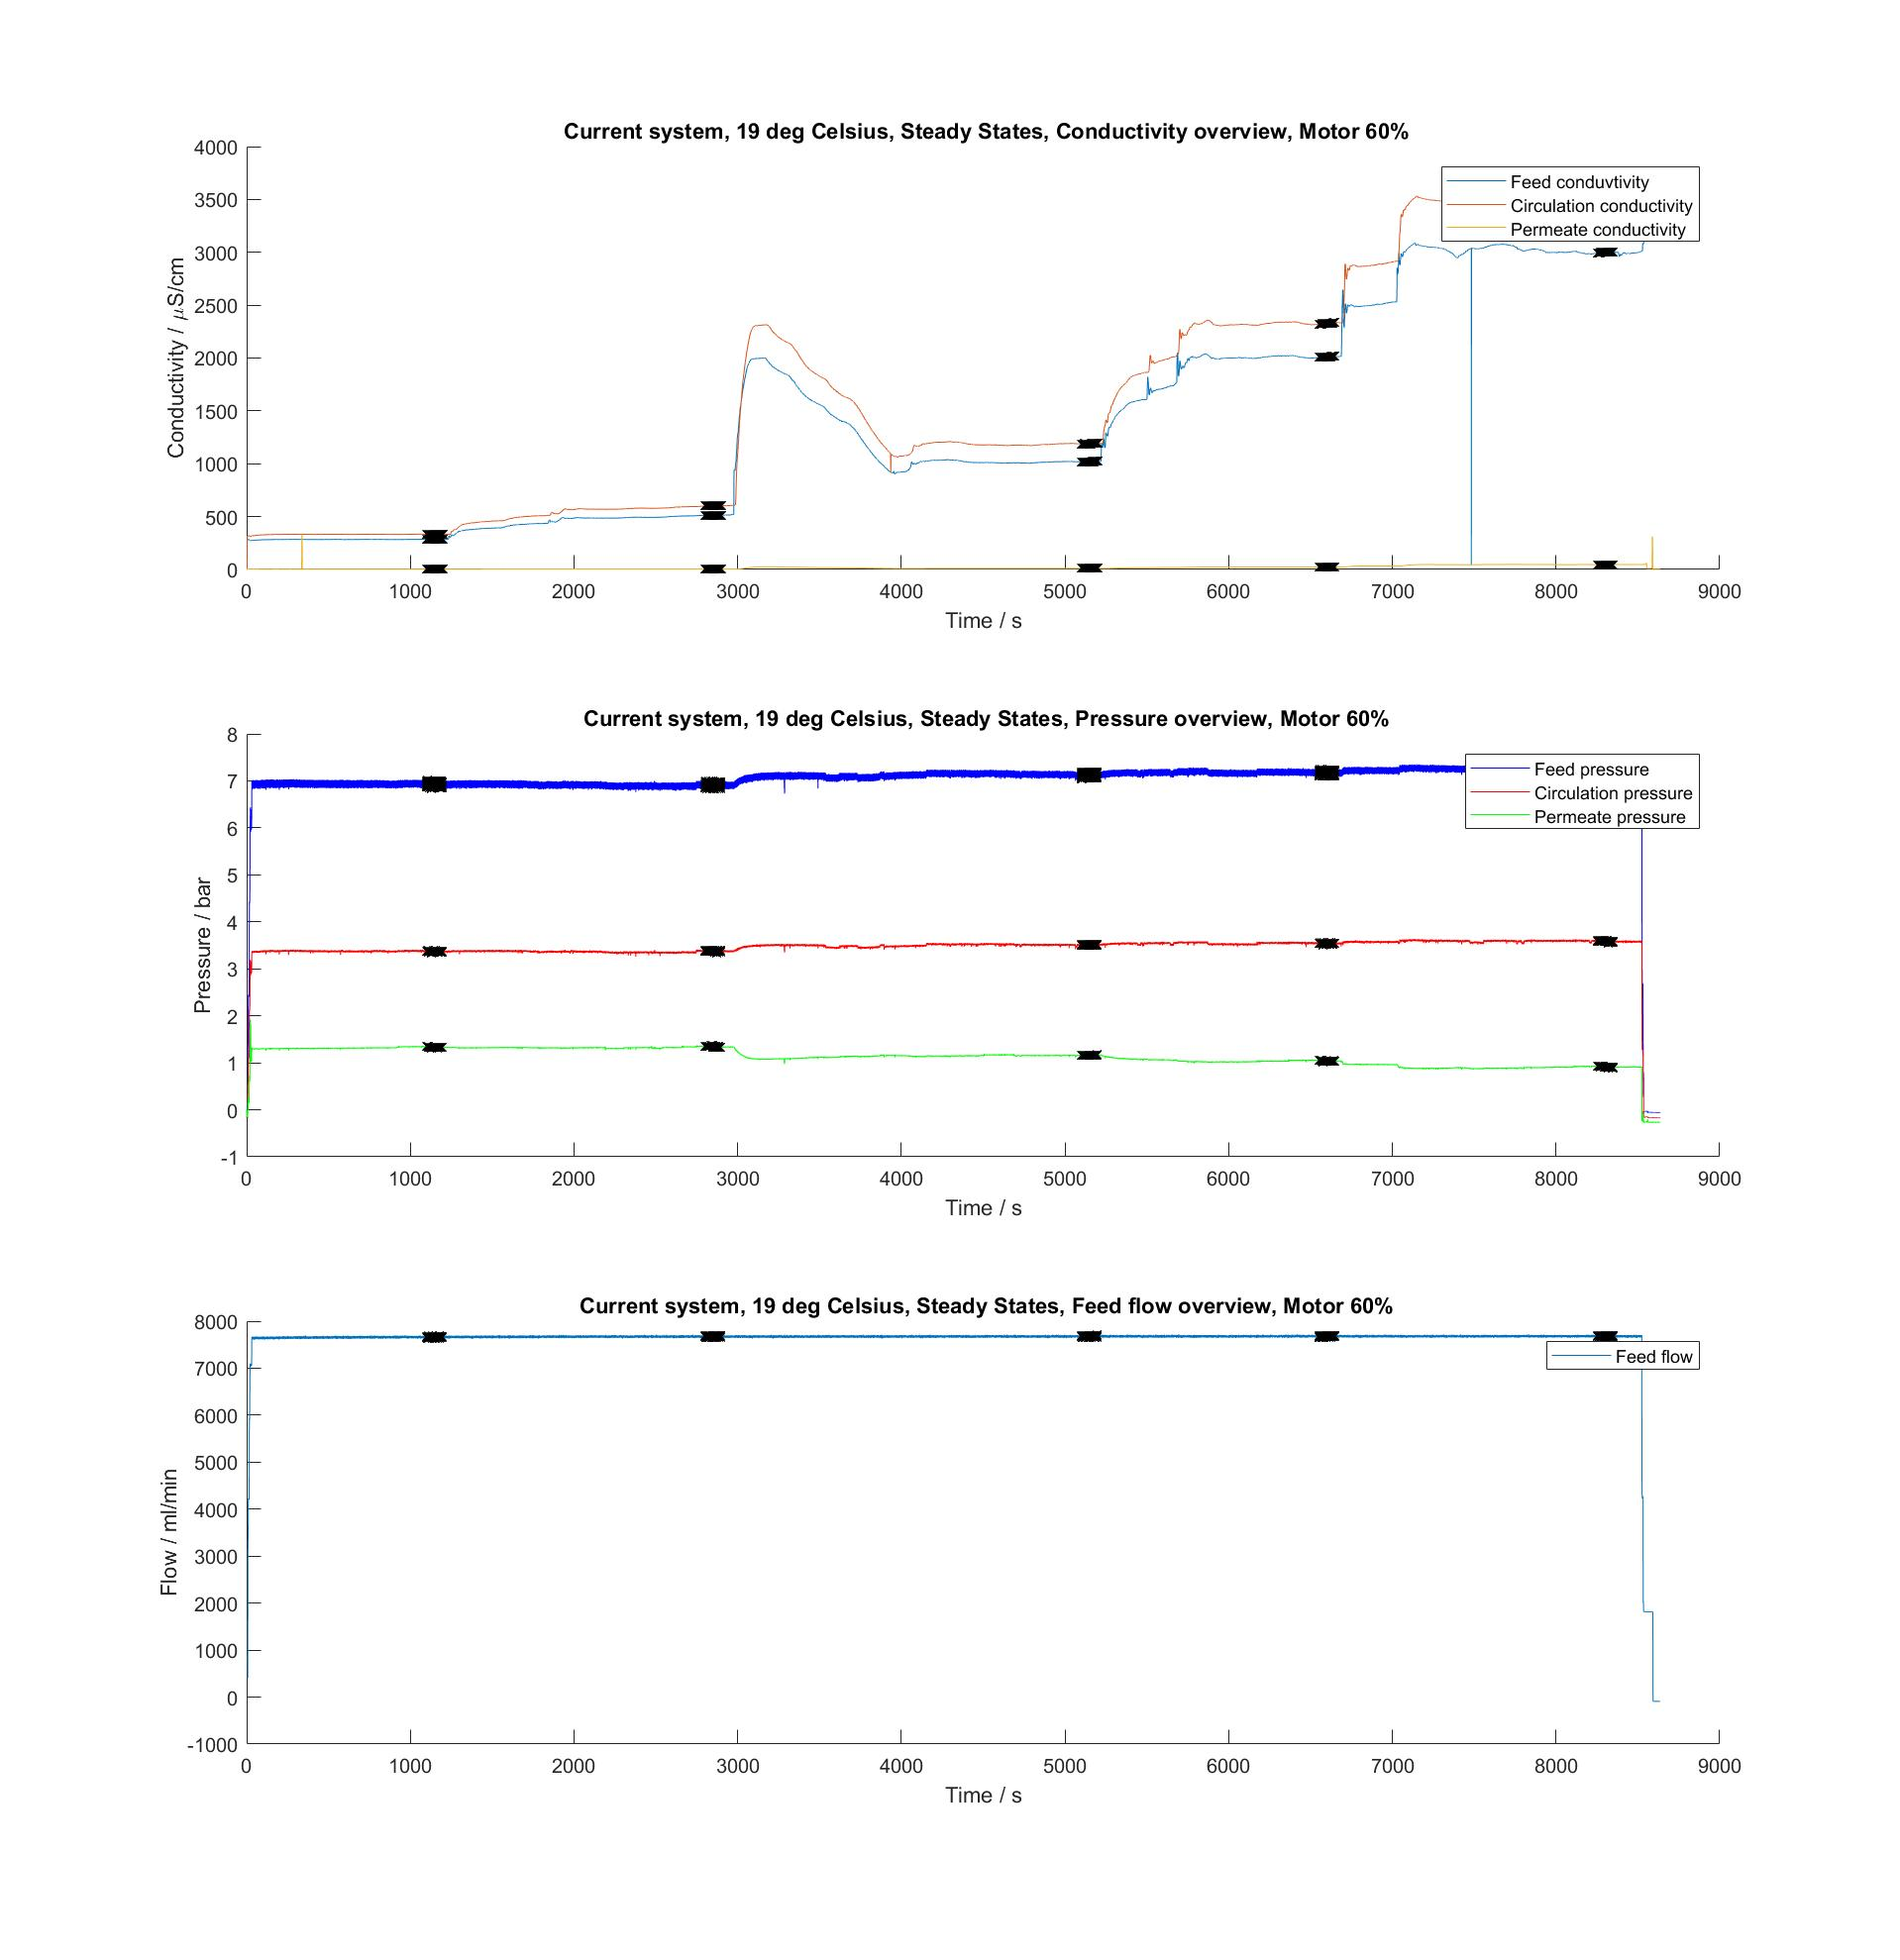
\includegraphics[width=1.1\textwidth]{overview20_60}
    \caption{Test 1, Current system, 18 degrees celsius. Steady states 1.1, 1.2, 1.3, 1.5 and 1.7 }
    \label{fig:PressConn}
\end{figure}

\newpage

\subsection{Current system, Test sequence 1, part 2}
  
\begin{figure}[H]
    \centering
    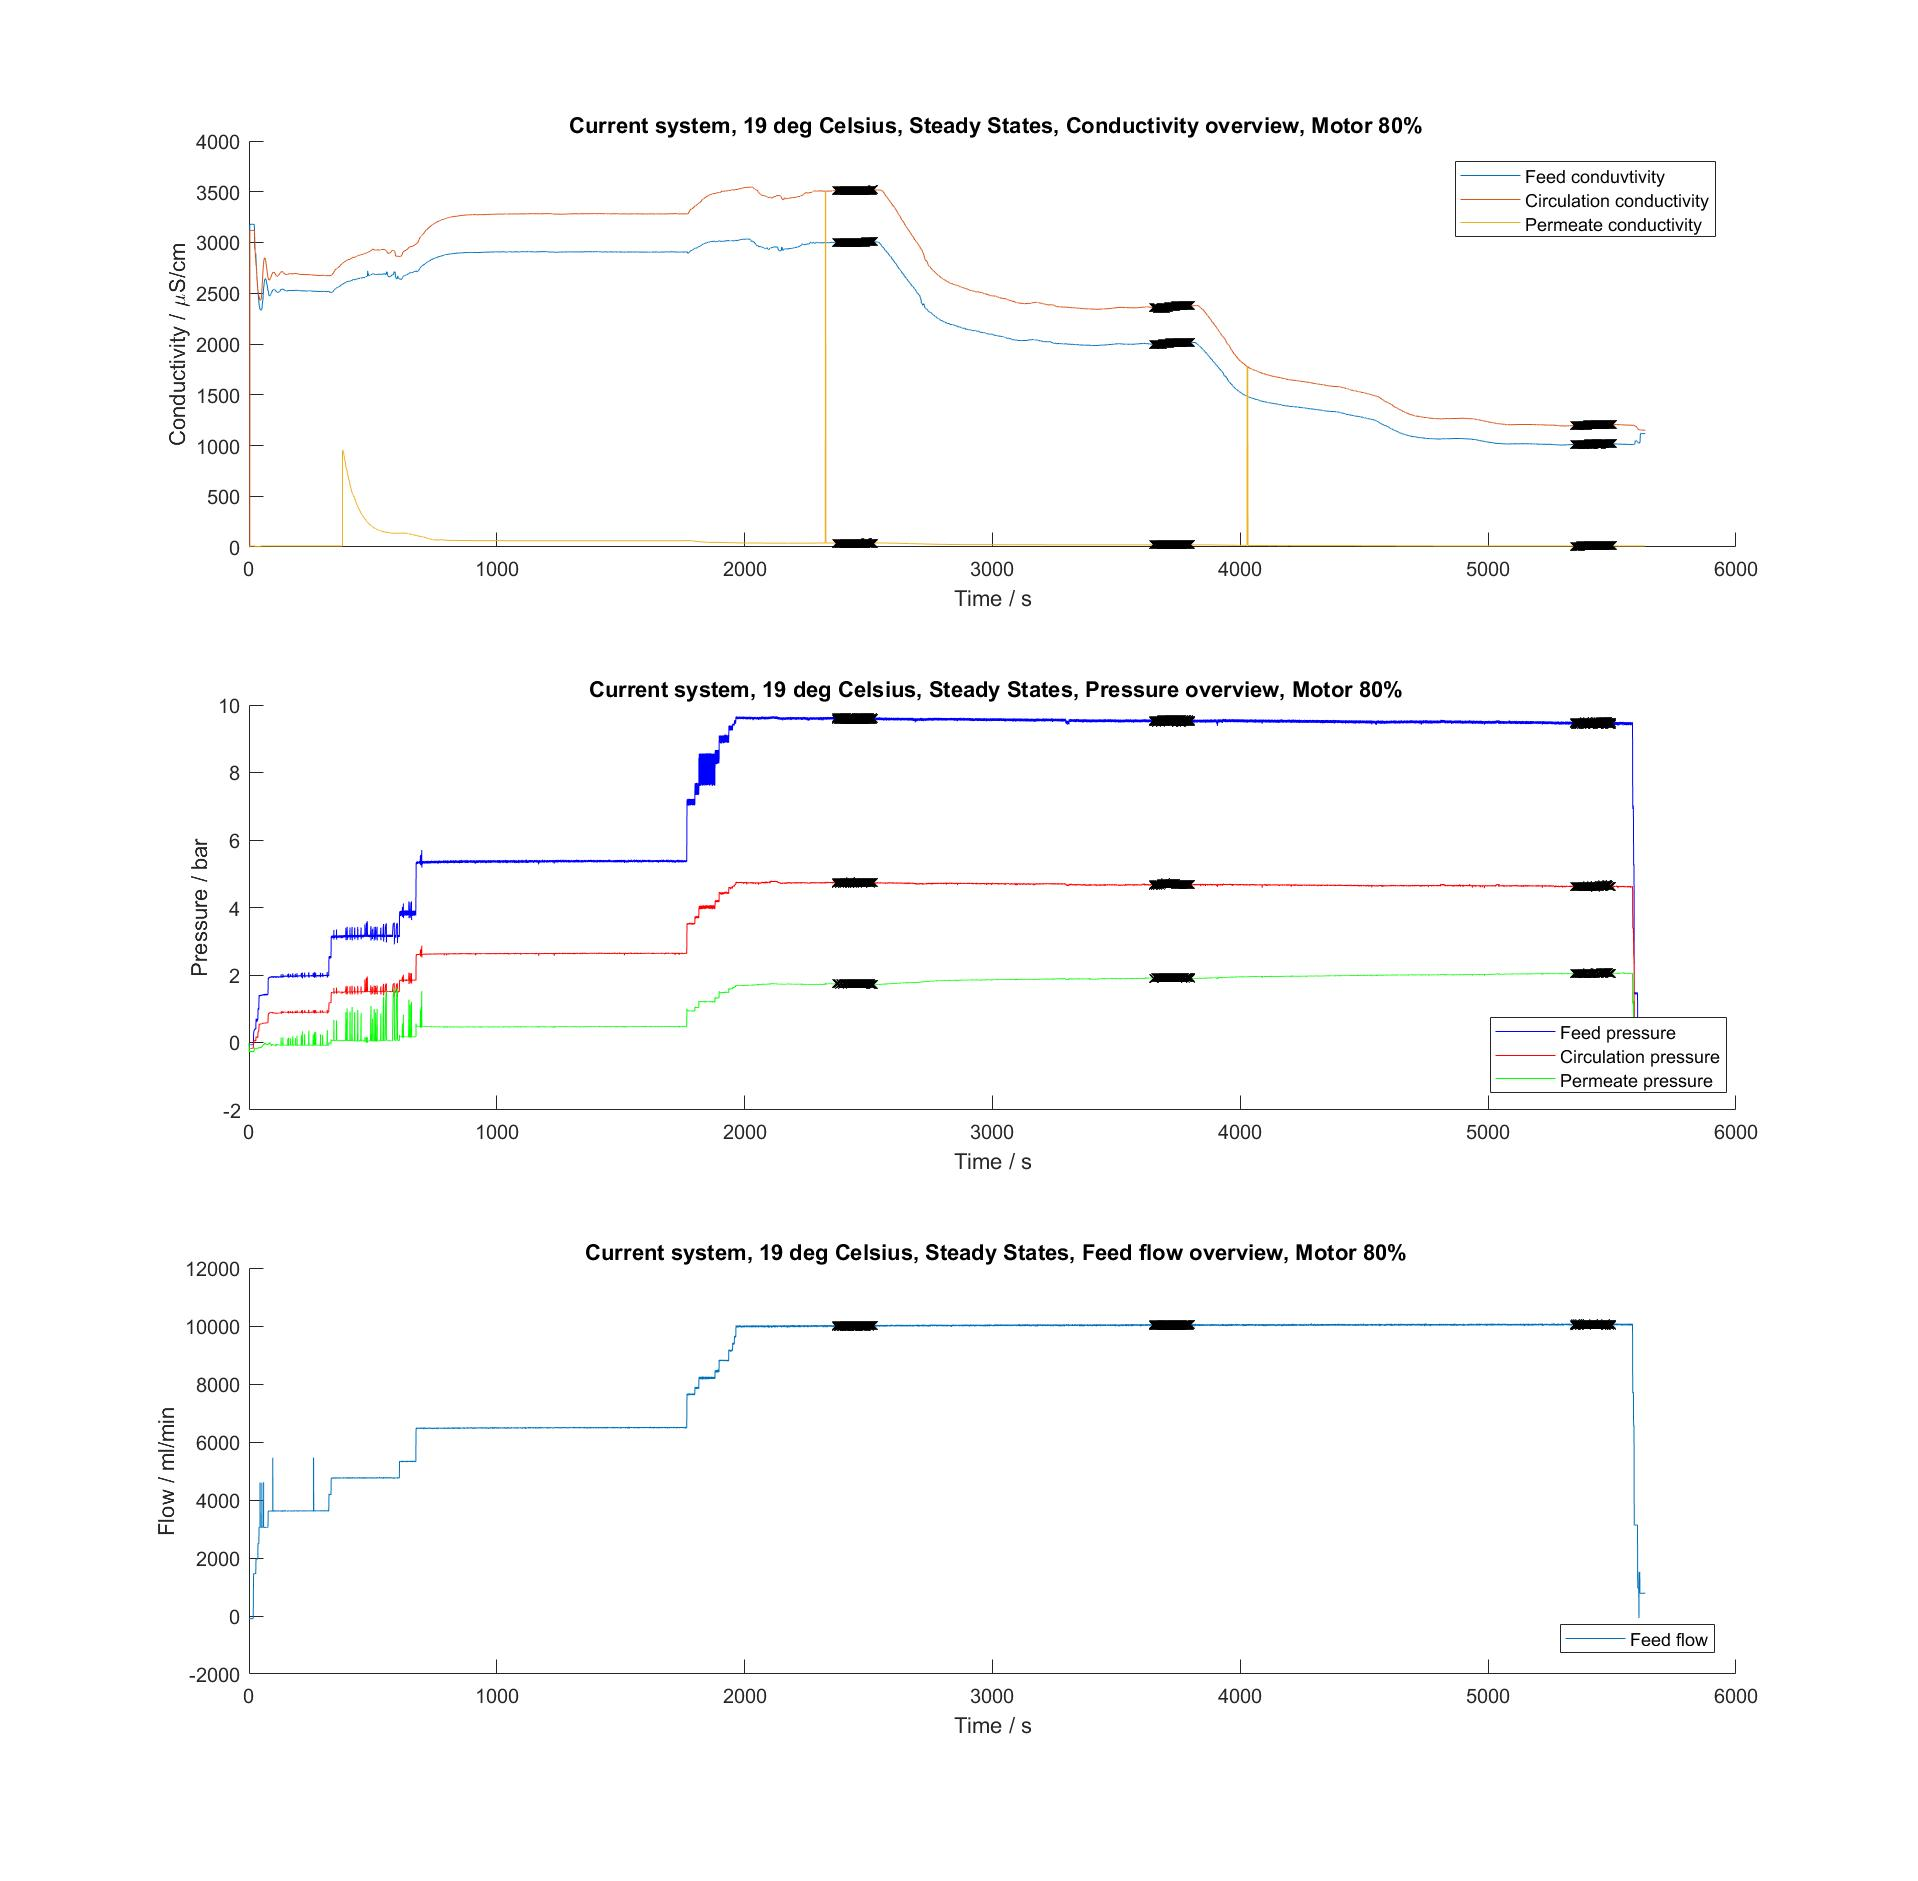
\includegraphics[width=1.1\textwidth]{overview20_80}
    \caption{Test 1, Current system, 18 degrees celsius. Steady states 1.4, 1.6 and 1.8}
    \label{fig:PressConn}
\end{figure}

\newpage

By post-proccesing the data from test one in Matlab it was possible to visually show how the system parameters were affected by the changed pump speed and feed conductivity. 


insert table, results on how the different graphs changed!!!

\begin{figure}[H]
    \centering
    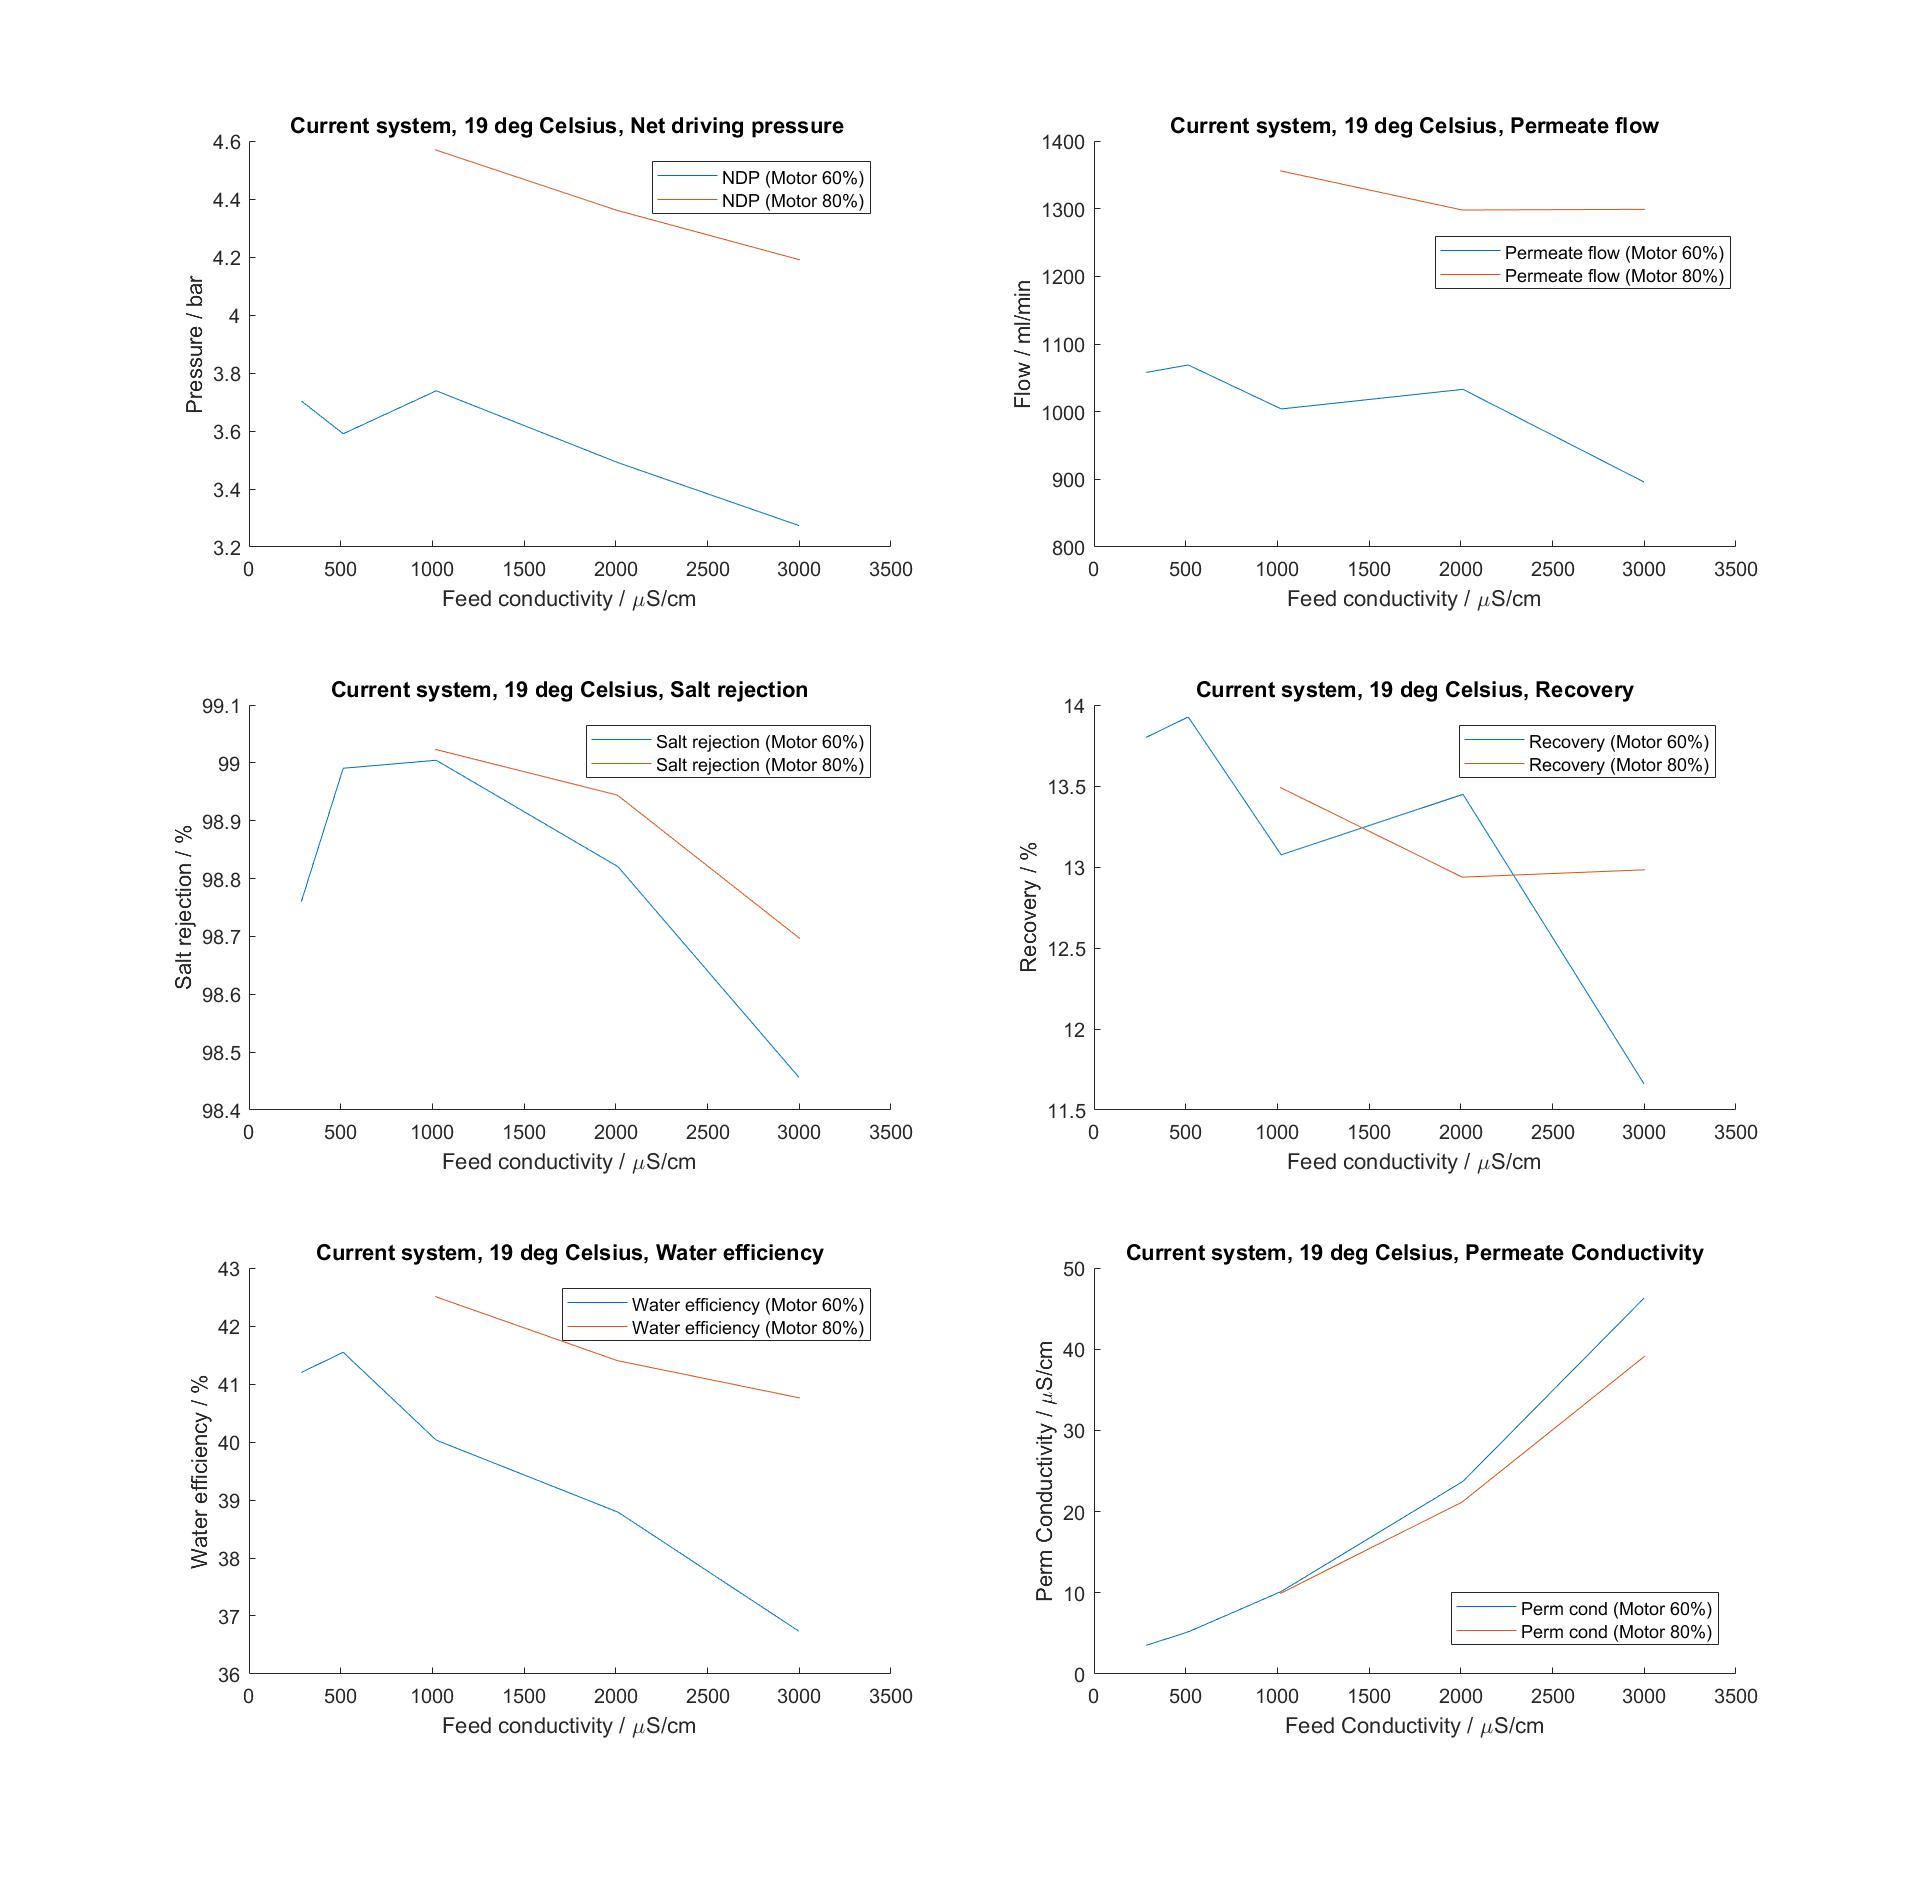
\includegraphics[width=1.1\textwidth]{Key20}
    \caption{Caption missing}
    \label{fig:PressConn}
\end{figure}

\newpage

\subsection{Current system, Test sequence 2}

The second test was carried out by setting the heater bath to 30 degrees celsius and and adjusting the conductivity and pump speed according to the test plan. Since the water was much warmer than the air in the room, the heating caused by the pump was not as prominent and allowed all steady states to be examined in one continous test.

\begin{figure}[H]
    \centering
    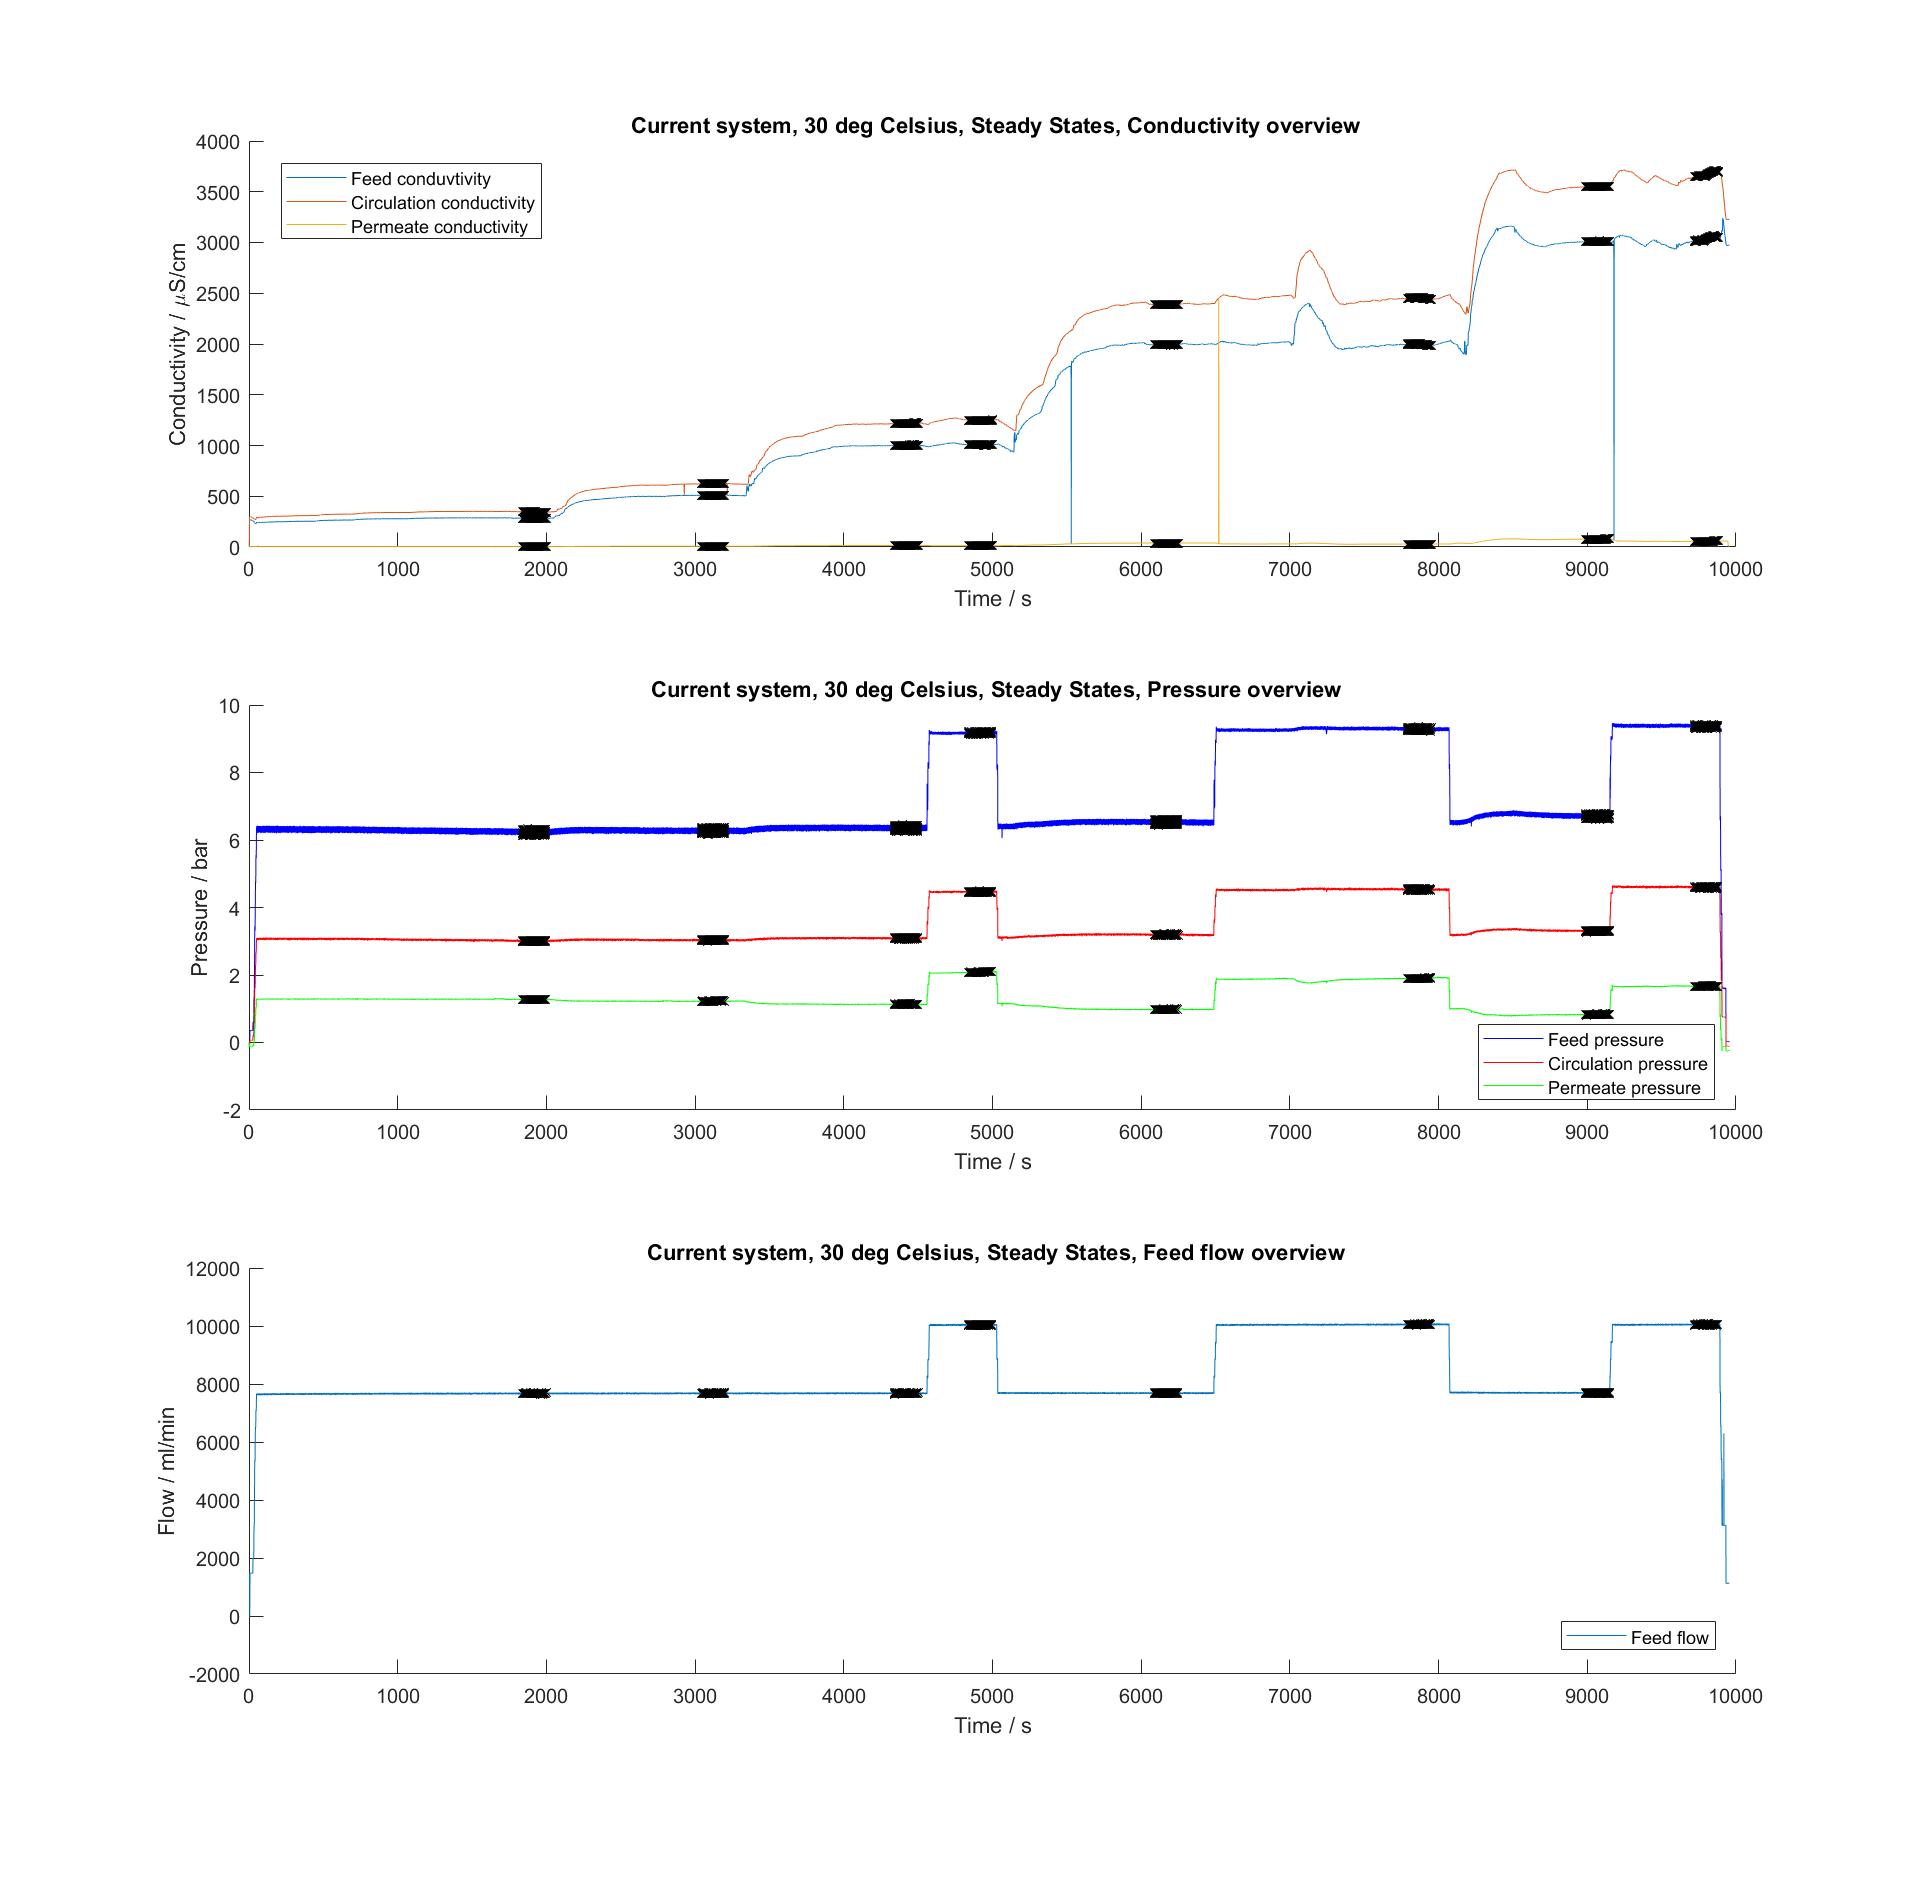
\includegraphics[width=1.1\textwidth]{overview30}
    \caption{Test 2, Current system, 30 degrees celsius. Steady states 1.1, 1.2, 1.3, 1.4 1.5, 1.6, 1.7 and 1.8}
    \label{fig:PressConn}
\end{figure}

\newpage


The data from the test was post processed in Matlab in exactly the same way as the previous test.

\begin{figure}[H]
    \centering
    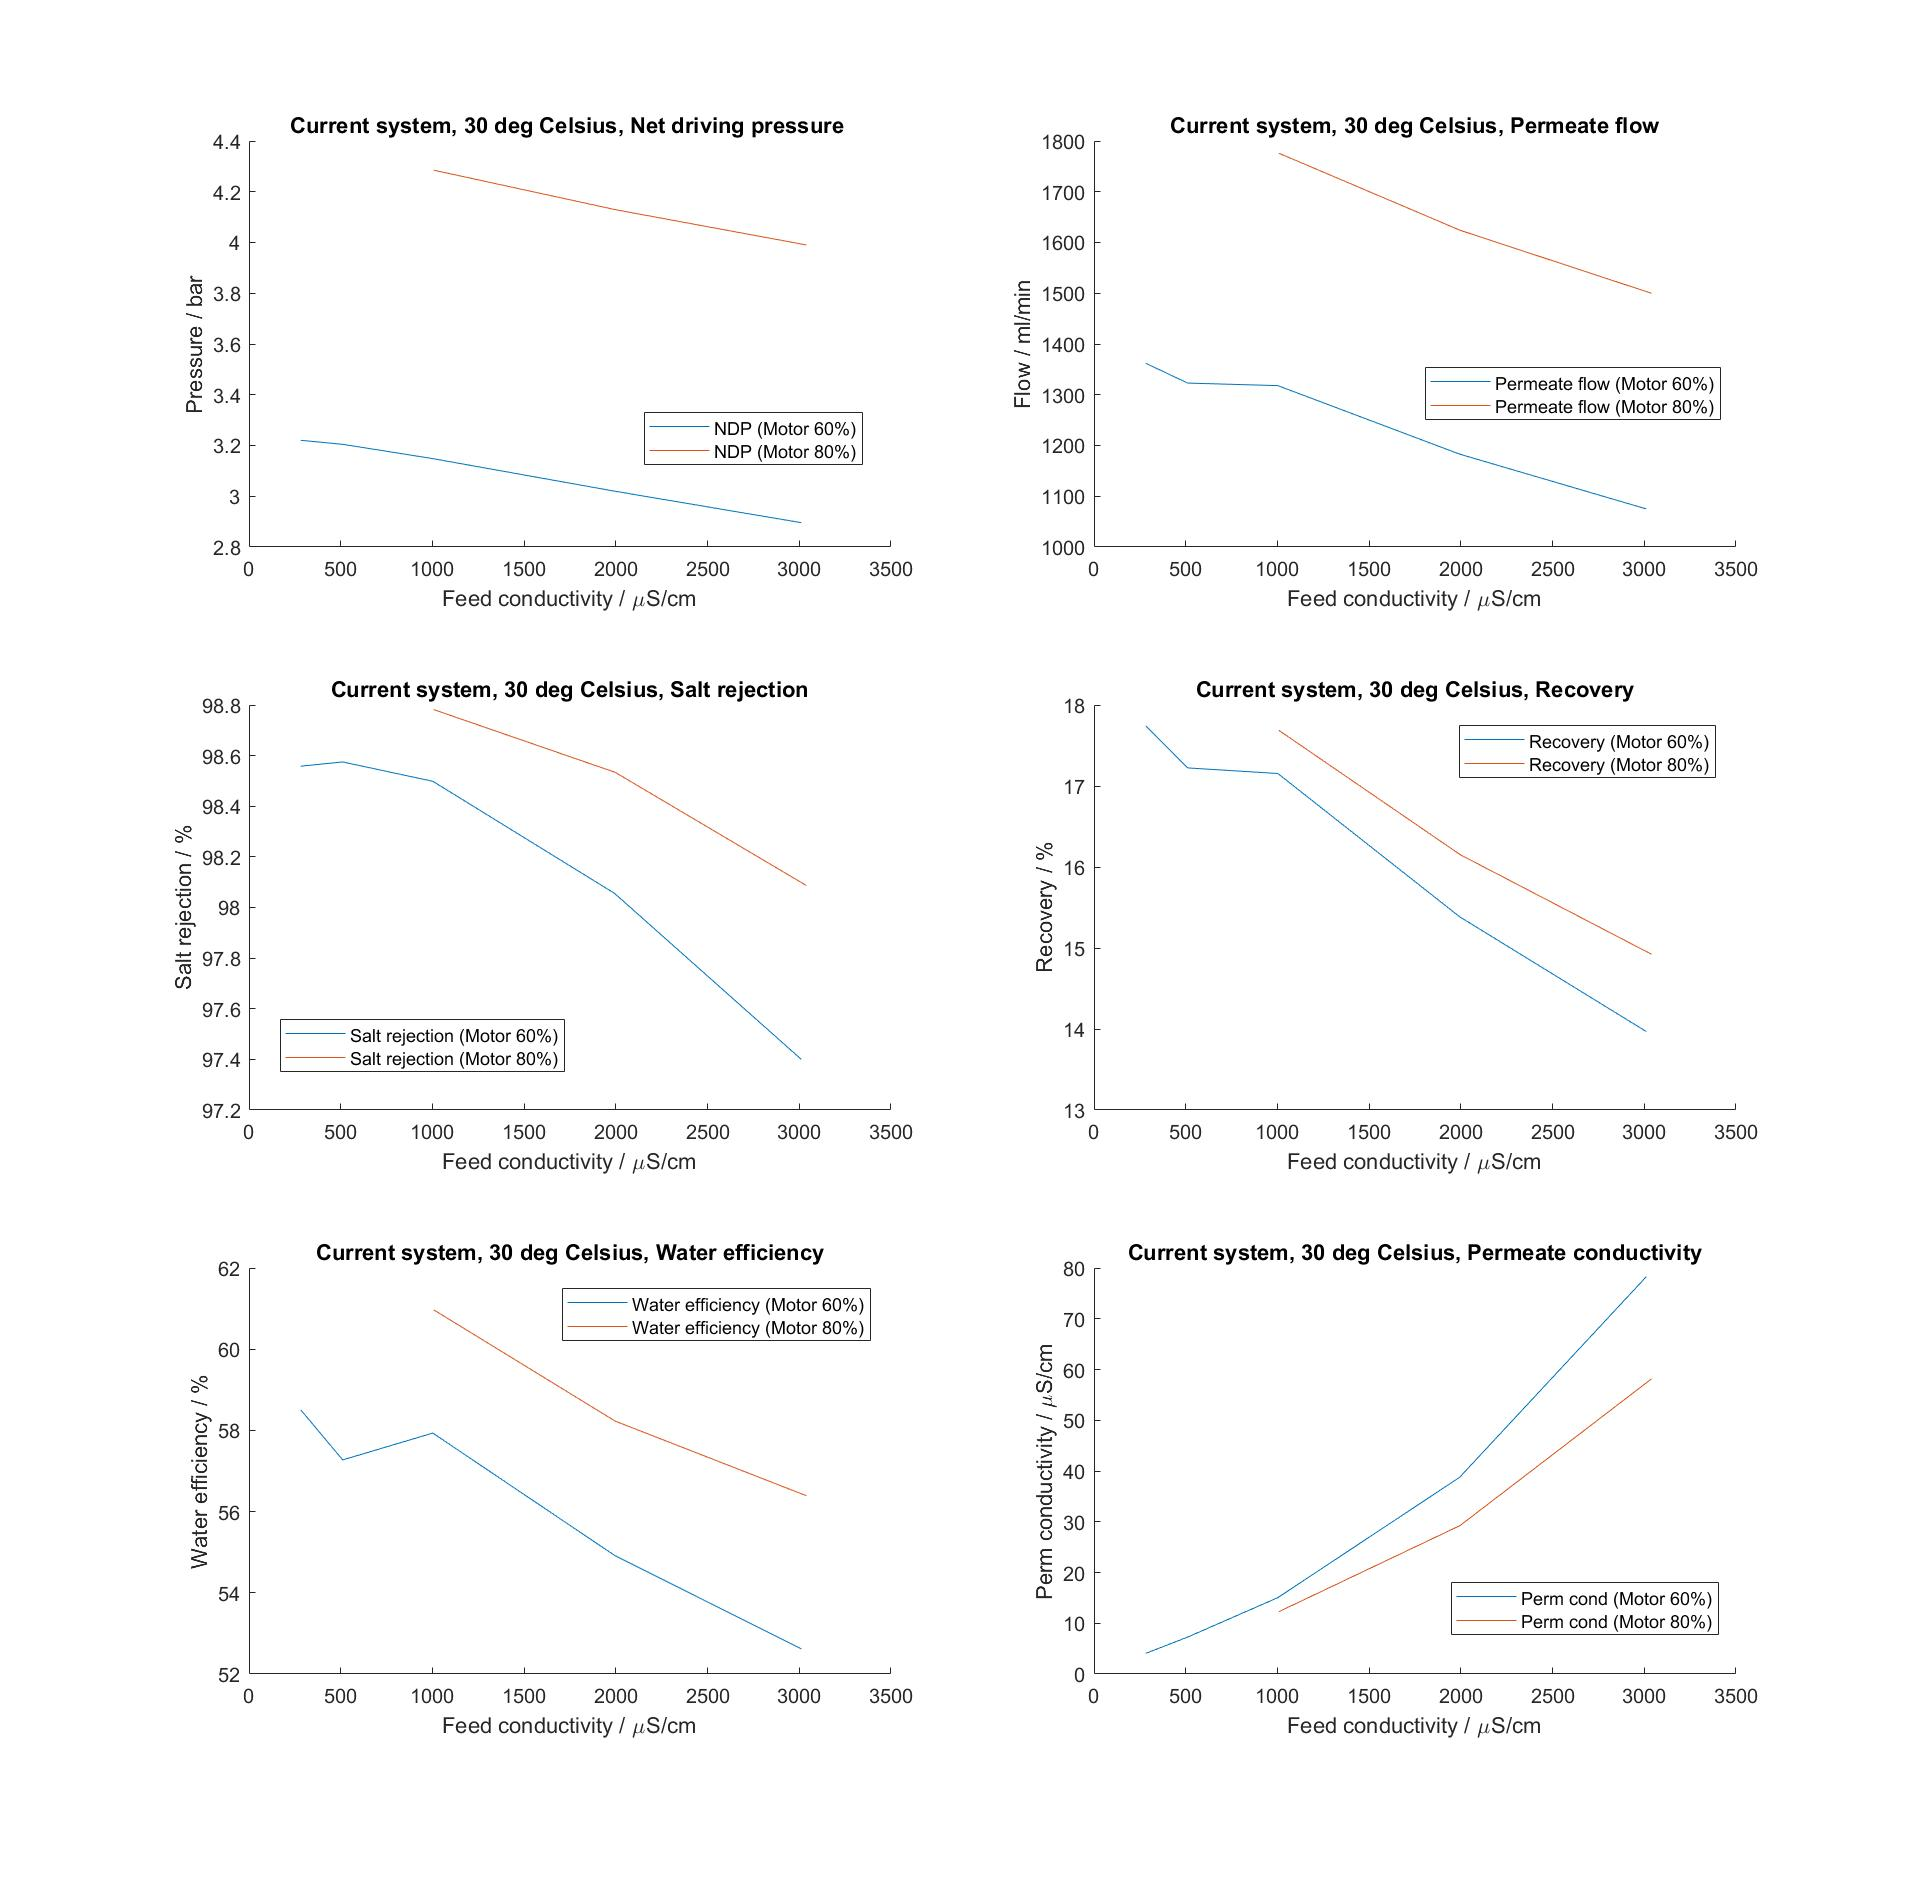
\includegraphics[width=1.1\textwidth]{Key30}
    \caption{Caption missing}
    \label{fig:PressConn}
\end{figure}

\newpage

\subsection{Current system, Test sequence 3}

Finally the heating bath was set to 40 C and the test sequence was performed just like test sequence 2. 

\begin{figure}[H]
    \centering
    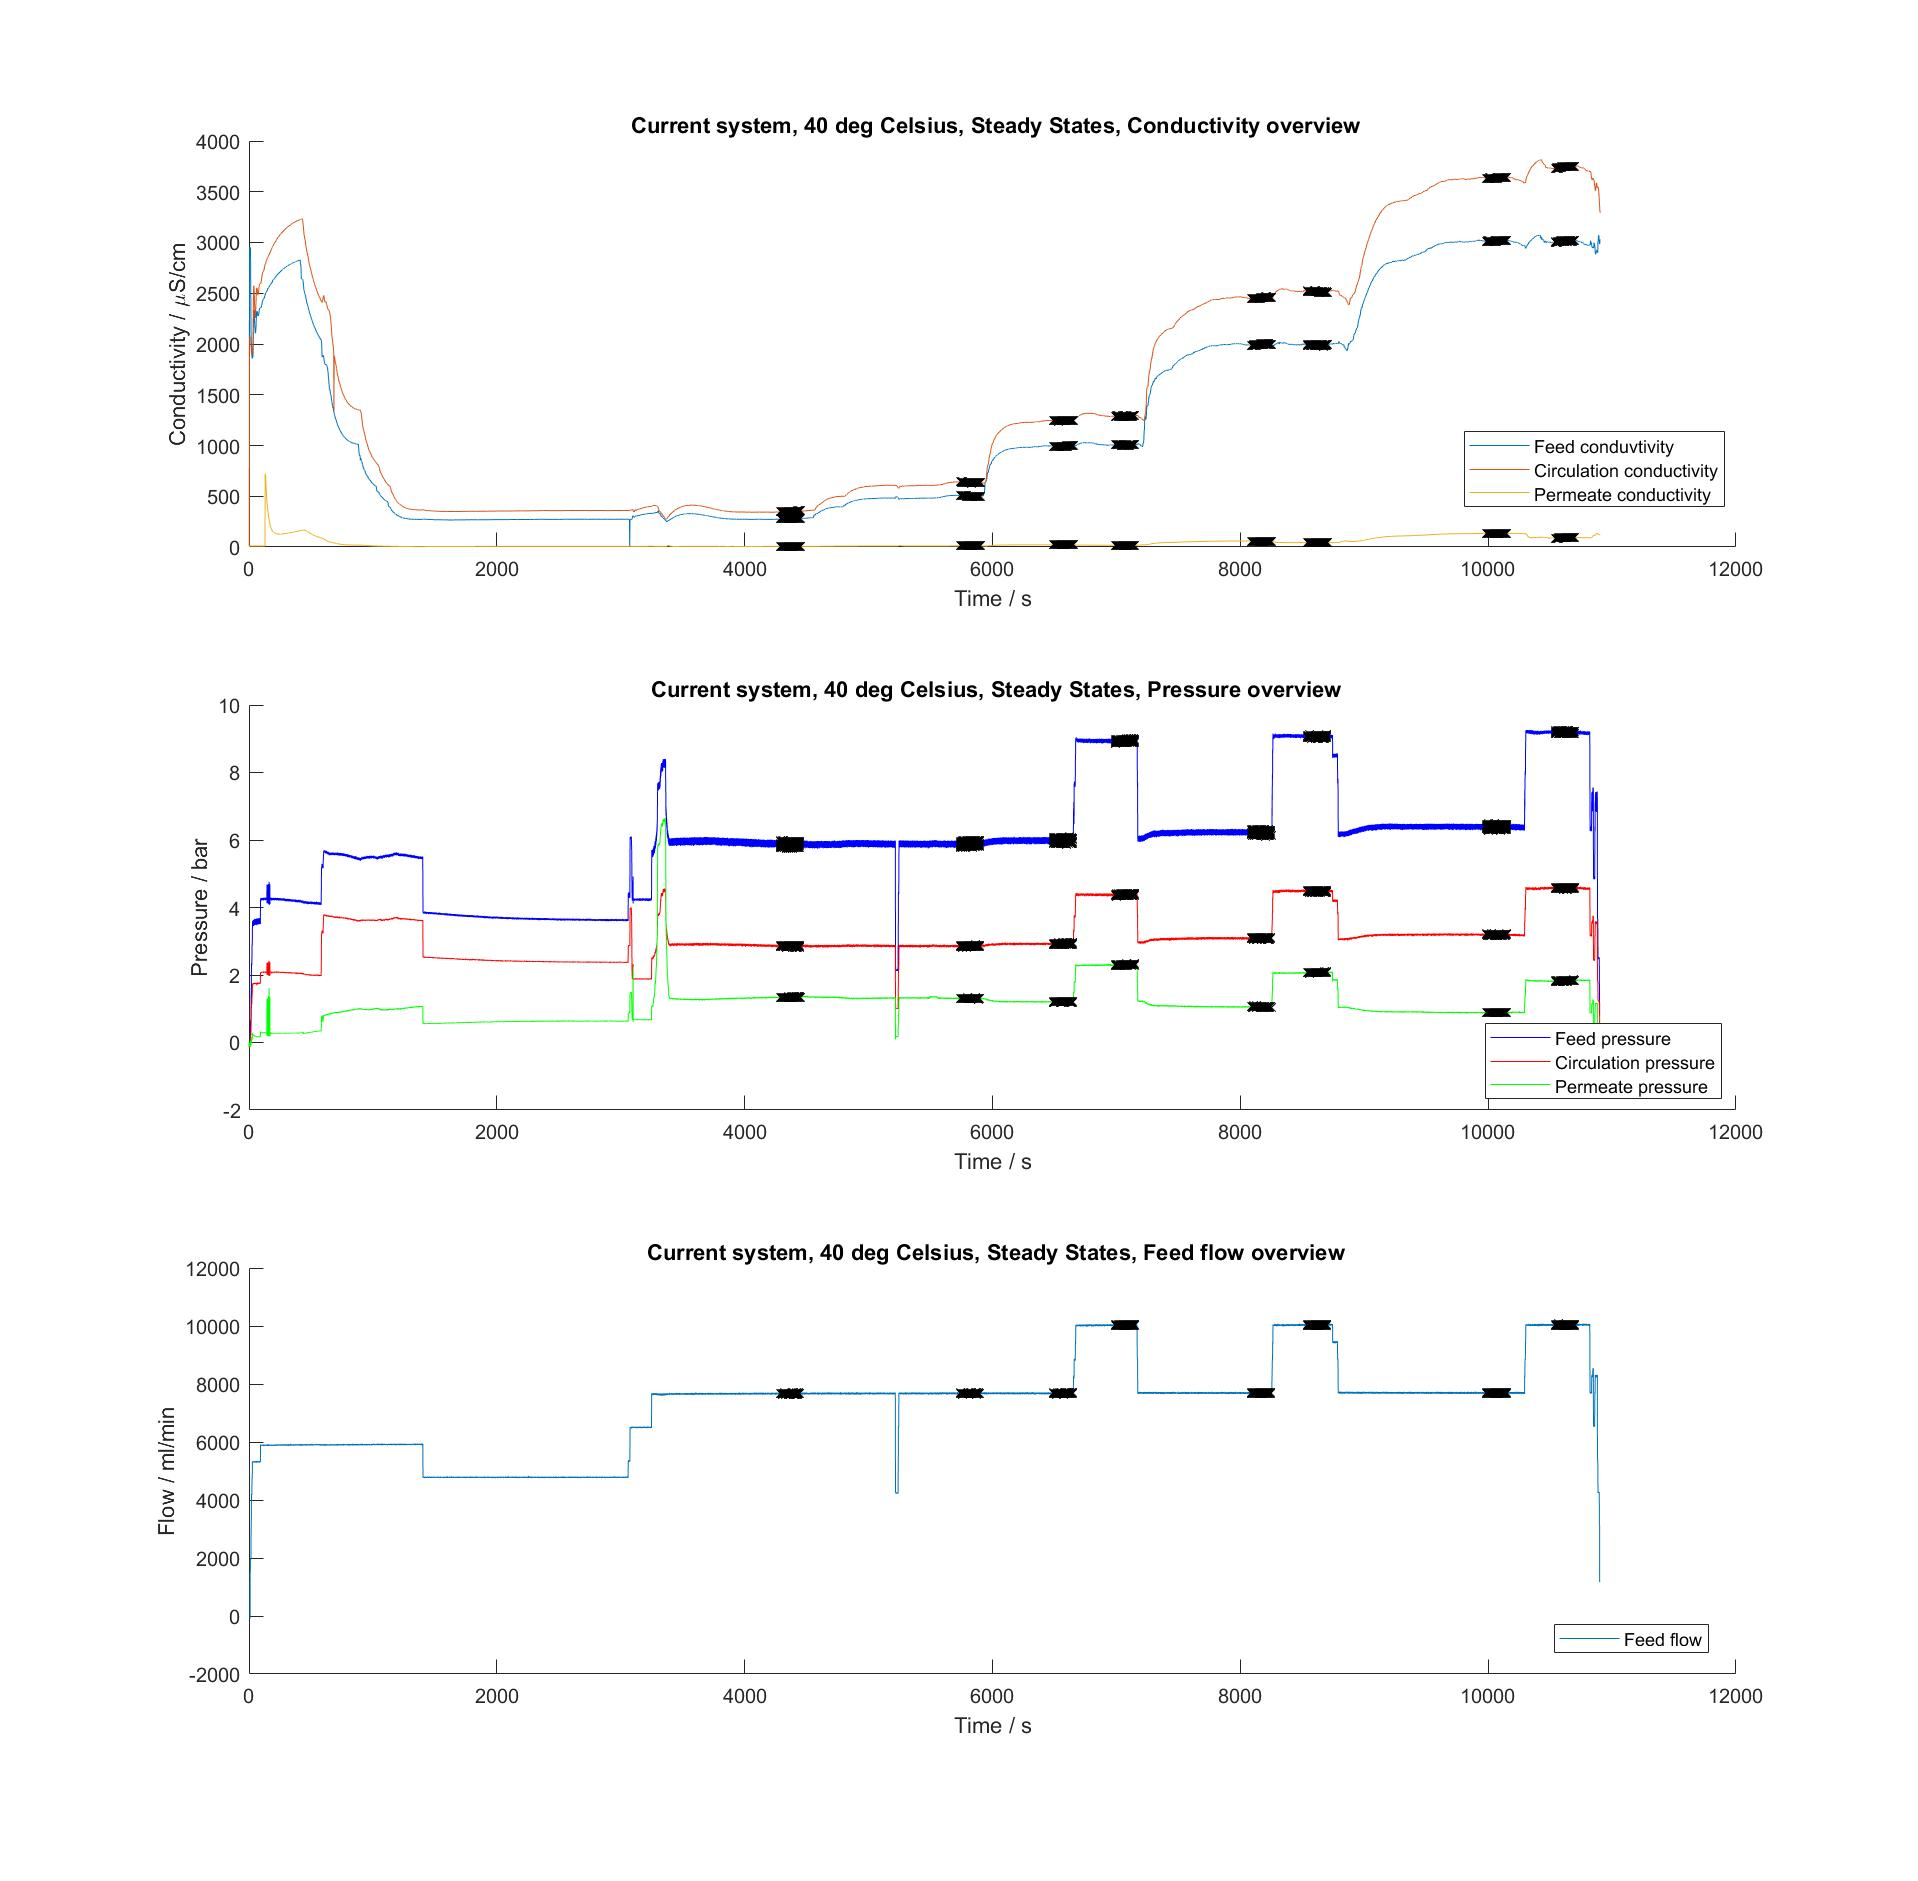
\includegraphics[width=1.1\textwidth]{overview40}
    \caption{Caption missing}
    \label{fig:PressConn}
\end{figure}

\newpage

Post processing in matlab generated the following data from the steady states.

\begin{figure}[H]
    \centering
    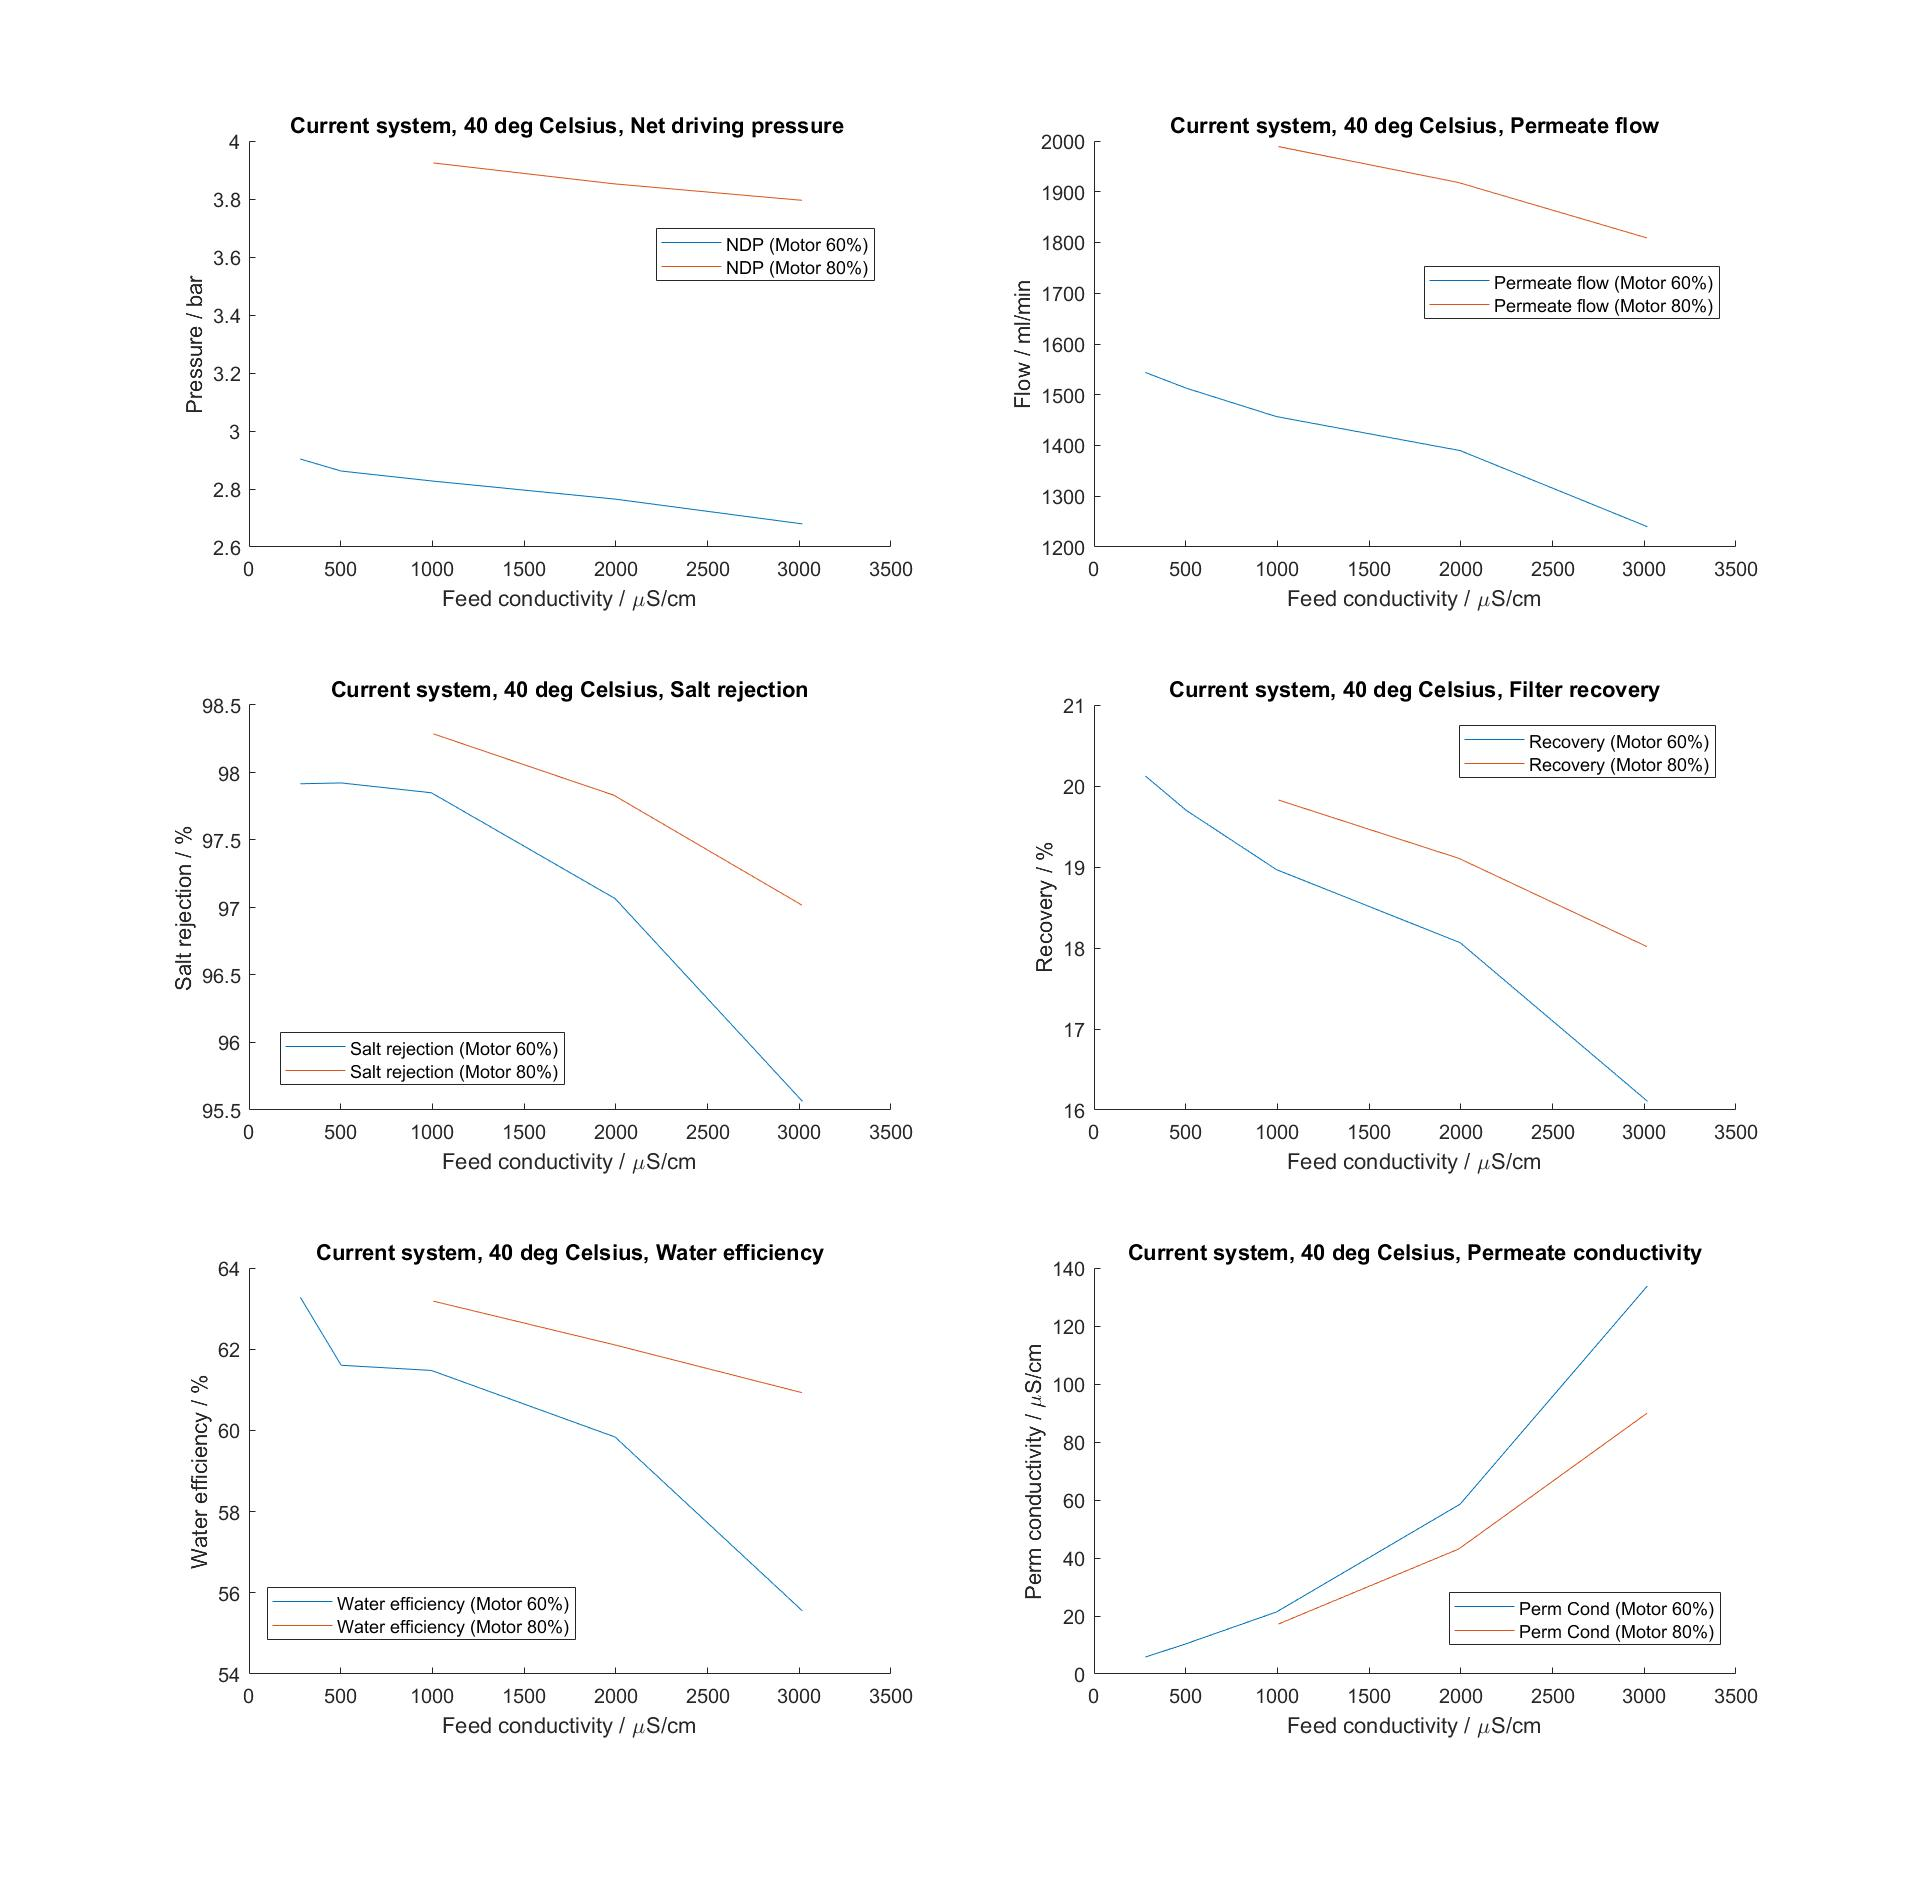
\includegraphics[width=1.1\textwidth]{Key40}
    \caption{Caption missing}
    \label{fig:PressConn}
\end{figure}

\newpage

In order to understand how the system current performed in different working conditions all plots from the post processing in Matlab was put togheter. 

\subsection{Net driving pressure}

Net driving pressure was decreased when the temperature was increased. Higher feed conductivity resulted in a decreased net driving pressure. As expected, running the feed pump at a higher RPM also increased the net driving pressure.

\begin{figure}[H]
    \centering
    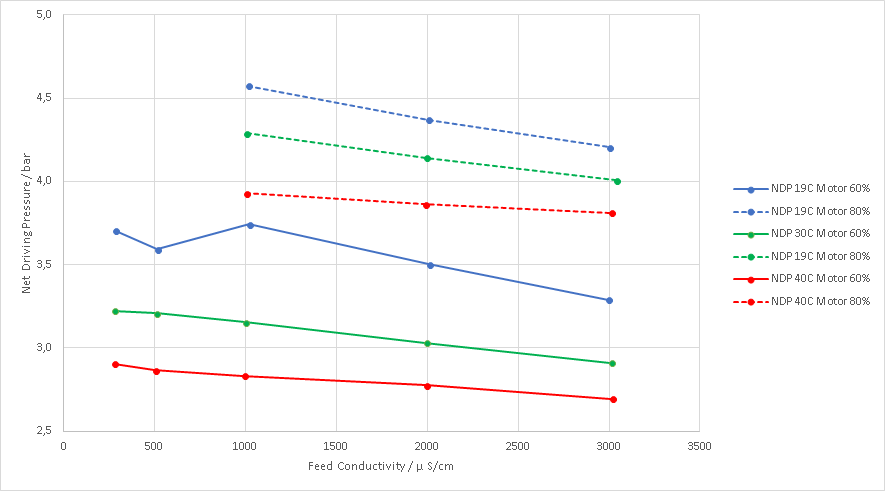
\includegraphics[width=0.8\textwidth]{NDP}
    \caption{Net driving pressure}
    \label{fig:NDP}
\end{figure}

\subsection{Permeate flow}

According to theory, Net driving pressure has a direct effect on permeate flow. When the feed pump was increased more water was pushed through the membrane. Increased water temperatures caused a much higher permeate flow. For instance, the permeate flow increased by around 50\% when the temperature was increased from 19 C to 40 C and the pump was running at 60\%. Due to the increased osmotic pressure, permeate flow decreased when the feed conductivity increased

\begin{figure}[H]
    \centering
    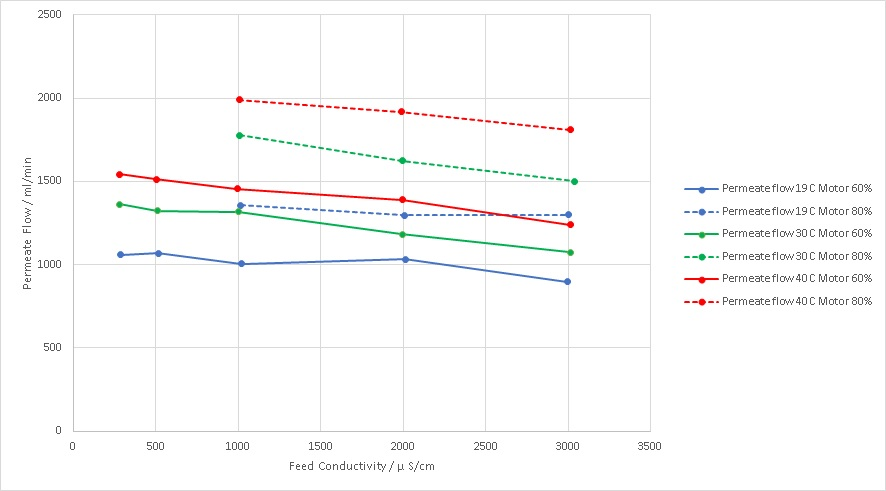
\includegraphics[width=0.8\textwidth]{permFlowCurrent}
    \caption{Caption missing}
    \label{fig:PressConn}
\end{figure}

\subsection{Recovery}

Warmer water enabled more feed water to pass through the membrane and therefore the recovery was increased. Increased conductivity reduced recovery due to the increased osmotic pressure.

\begin{figure}[H]
    \centering
    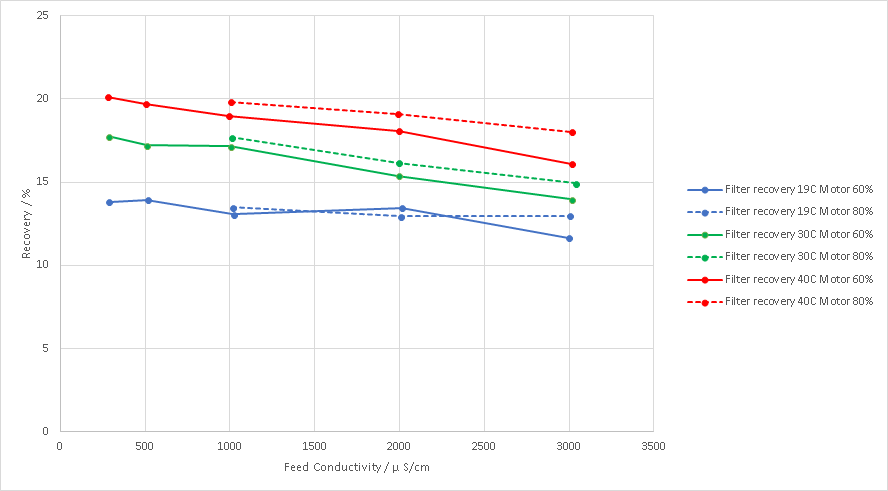
\includegraphics[width=0.8\textwidth]{Recovery}
    \caption{Caption missing}
    \label{fig:PressConn}
\end{figure}

\subsection{Salt rejection}

By looking at plot 5.13 the deterimental effects of both increased temperature and feed conductivity can be seen. The negative effect of increased feed conductivity was much more prominent at 40 C than 30C which means that the performance of the membrane decreased exponentially with higher temperature. Increased feed pump pressure resultet in better salt rejection and the positive effect of increased pump pressure was larger when the system was hot. Temperature was the parameter that decreased salt rejetion the most and by comparing how the system performed when the pump and feed conductivity was set to 60\% and 3000uS/cm at 19C and 40C it can be seen that the salt rejection decreased from 98.5\% to 95.5 \%. From the experiment it can also be concluded that the system perform much better at low temperature and feed conductivity that at high temperature and feed conductivity. 

\begin{figure}[H]
    \centering
    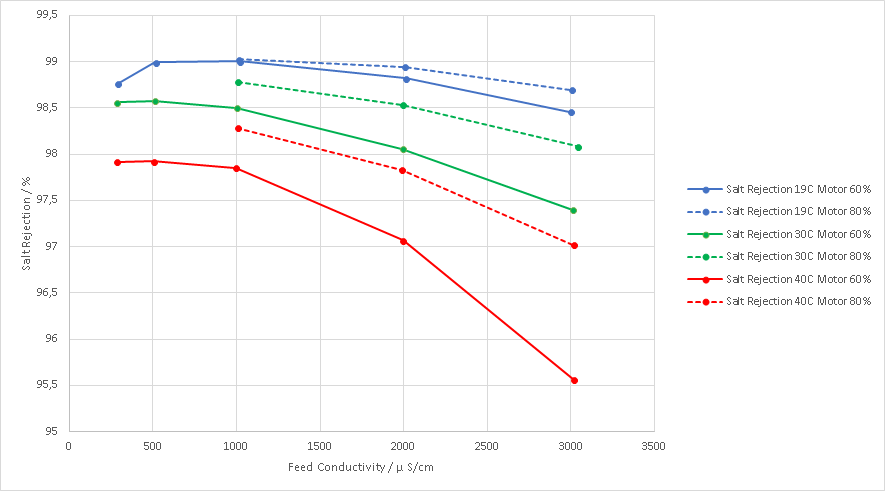
\includegraphics[width=0.8\textwidth]{SaltRejection}
    \caption{Saltrejection}
    \label{fig:SalrRejectionResult}
\end{figure}
 
\subsection{Permeate conductivity}

Permeate conductivity was directly proportional to salt rejection at a certain termperature and feed conductivity. The black line in plot 5.14 show the critical permeate conductivity that the system should be able to maintain and from the plot it is possible to se how high the conductivity can be in the recirculation loop without exceeding this limit. The operational area for the different temperature and pump pressure can be seen in plot TBD below.

\begin{figure}[H]
    \centering
    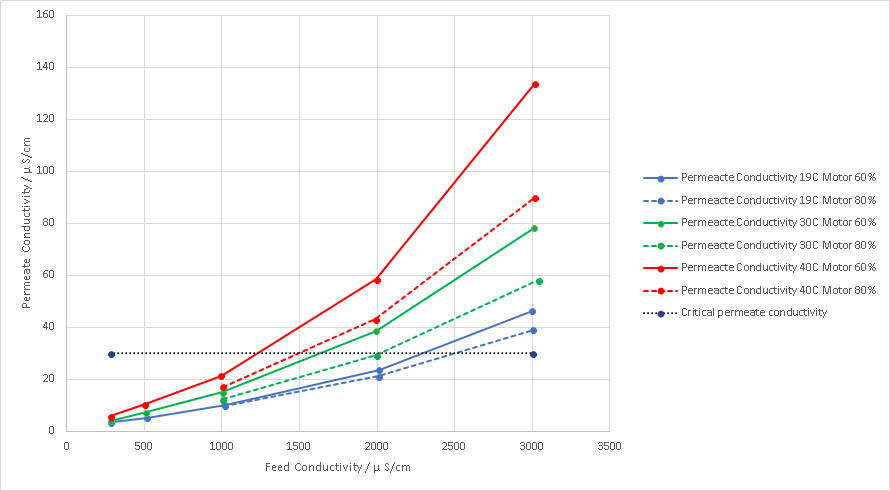
\includegraphics[width=0.8\textwidth]{PermCond}
    \caption{Conductivity}
    \label{fig:PressConn}
\end{figure}

!!INSERT TABLE!!

\subsection{Water efficiency}

Water efficiency increased when the temperature increased due to more permeate water being generated by the same feed pressure.

\begin{figure}[H]
    \centering
    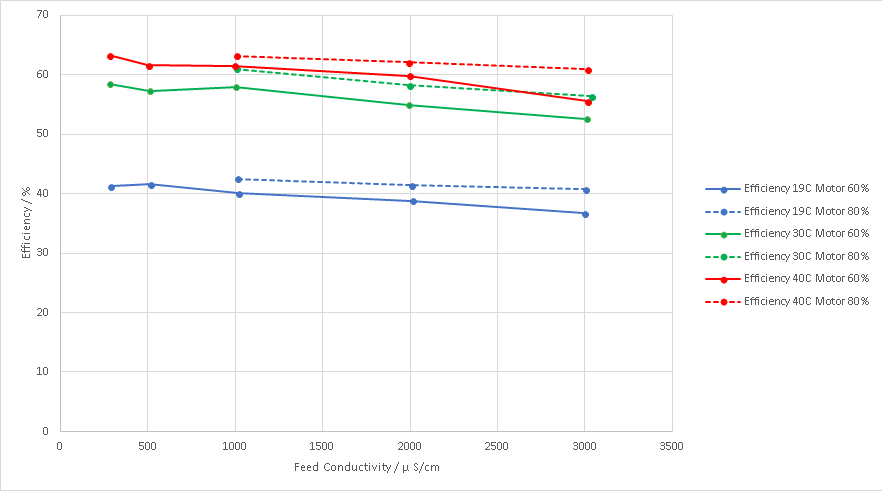
\includegraphics[width=0.8\textwidth]{Efficiency}
    \caption{Efficiency}
    \label{fig:PressConn}
\end{figure}

\newpage

\subsection{System 2}

The circulation pump and a flow meter was added to the system and the flow path was modified according to figure XXXX. The rig was also reprogrammed to be able to measure all flows in the flow path in real time. This could be done because now both the feed flow, circulation flow and permeate flow could be measured and from this data, the inlet and drain flow could be calculated. 


\newpage
\subsubsection{increased circulation}

The Initial idea for optimizing the membrane was to use the circulation pump to create a turbulent flow close to the membrane surface. Therefore, a test was set up to test this idea.
During the test, the feed pump and drain valve was set to a fixed value and the circulation pump was increased from 5\% to 35\%. Figure \ref{fig:RecIncrease} show the permeate conductivity, circulation flow and feed pressure and 7 steady state points from the test.

The circulation flow was increased from 1500 ml/min to 5000 ml/min and the increased circulation flow caused the pressure to increase from 5.5 to 7 bar. The permeate conductivity remained unchanged. 
\begin{figure}[H]
    \centering
    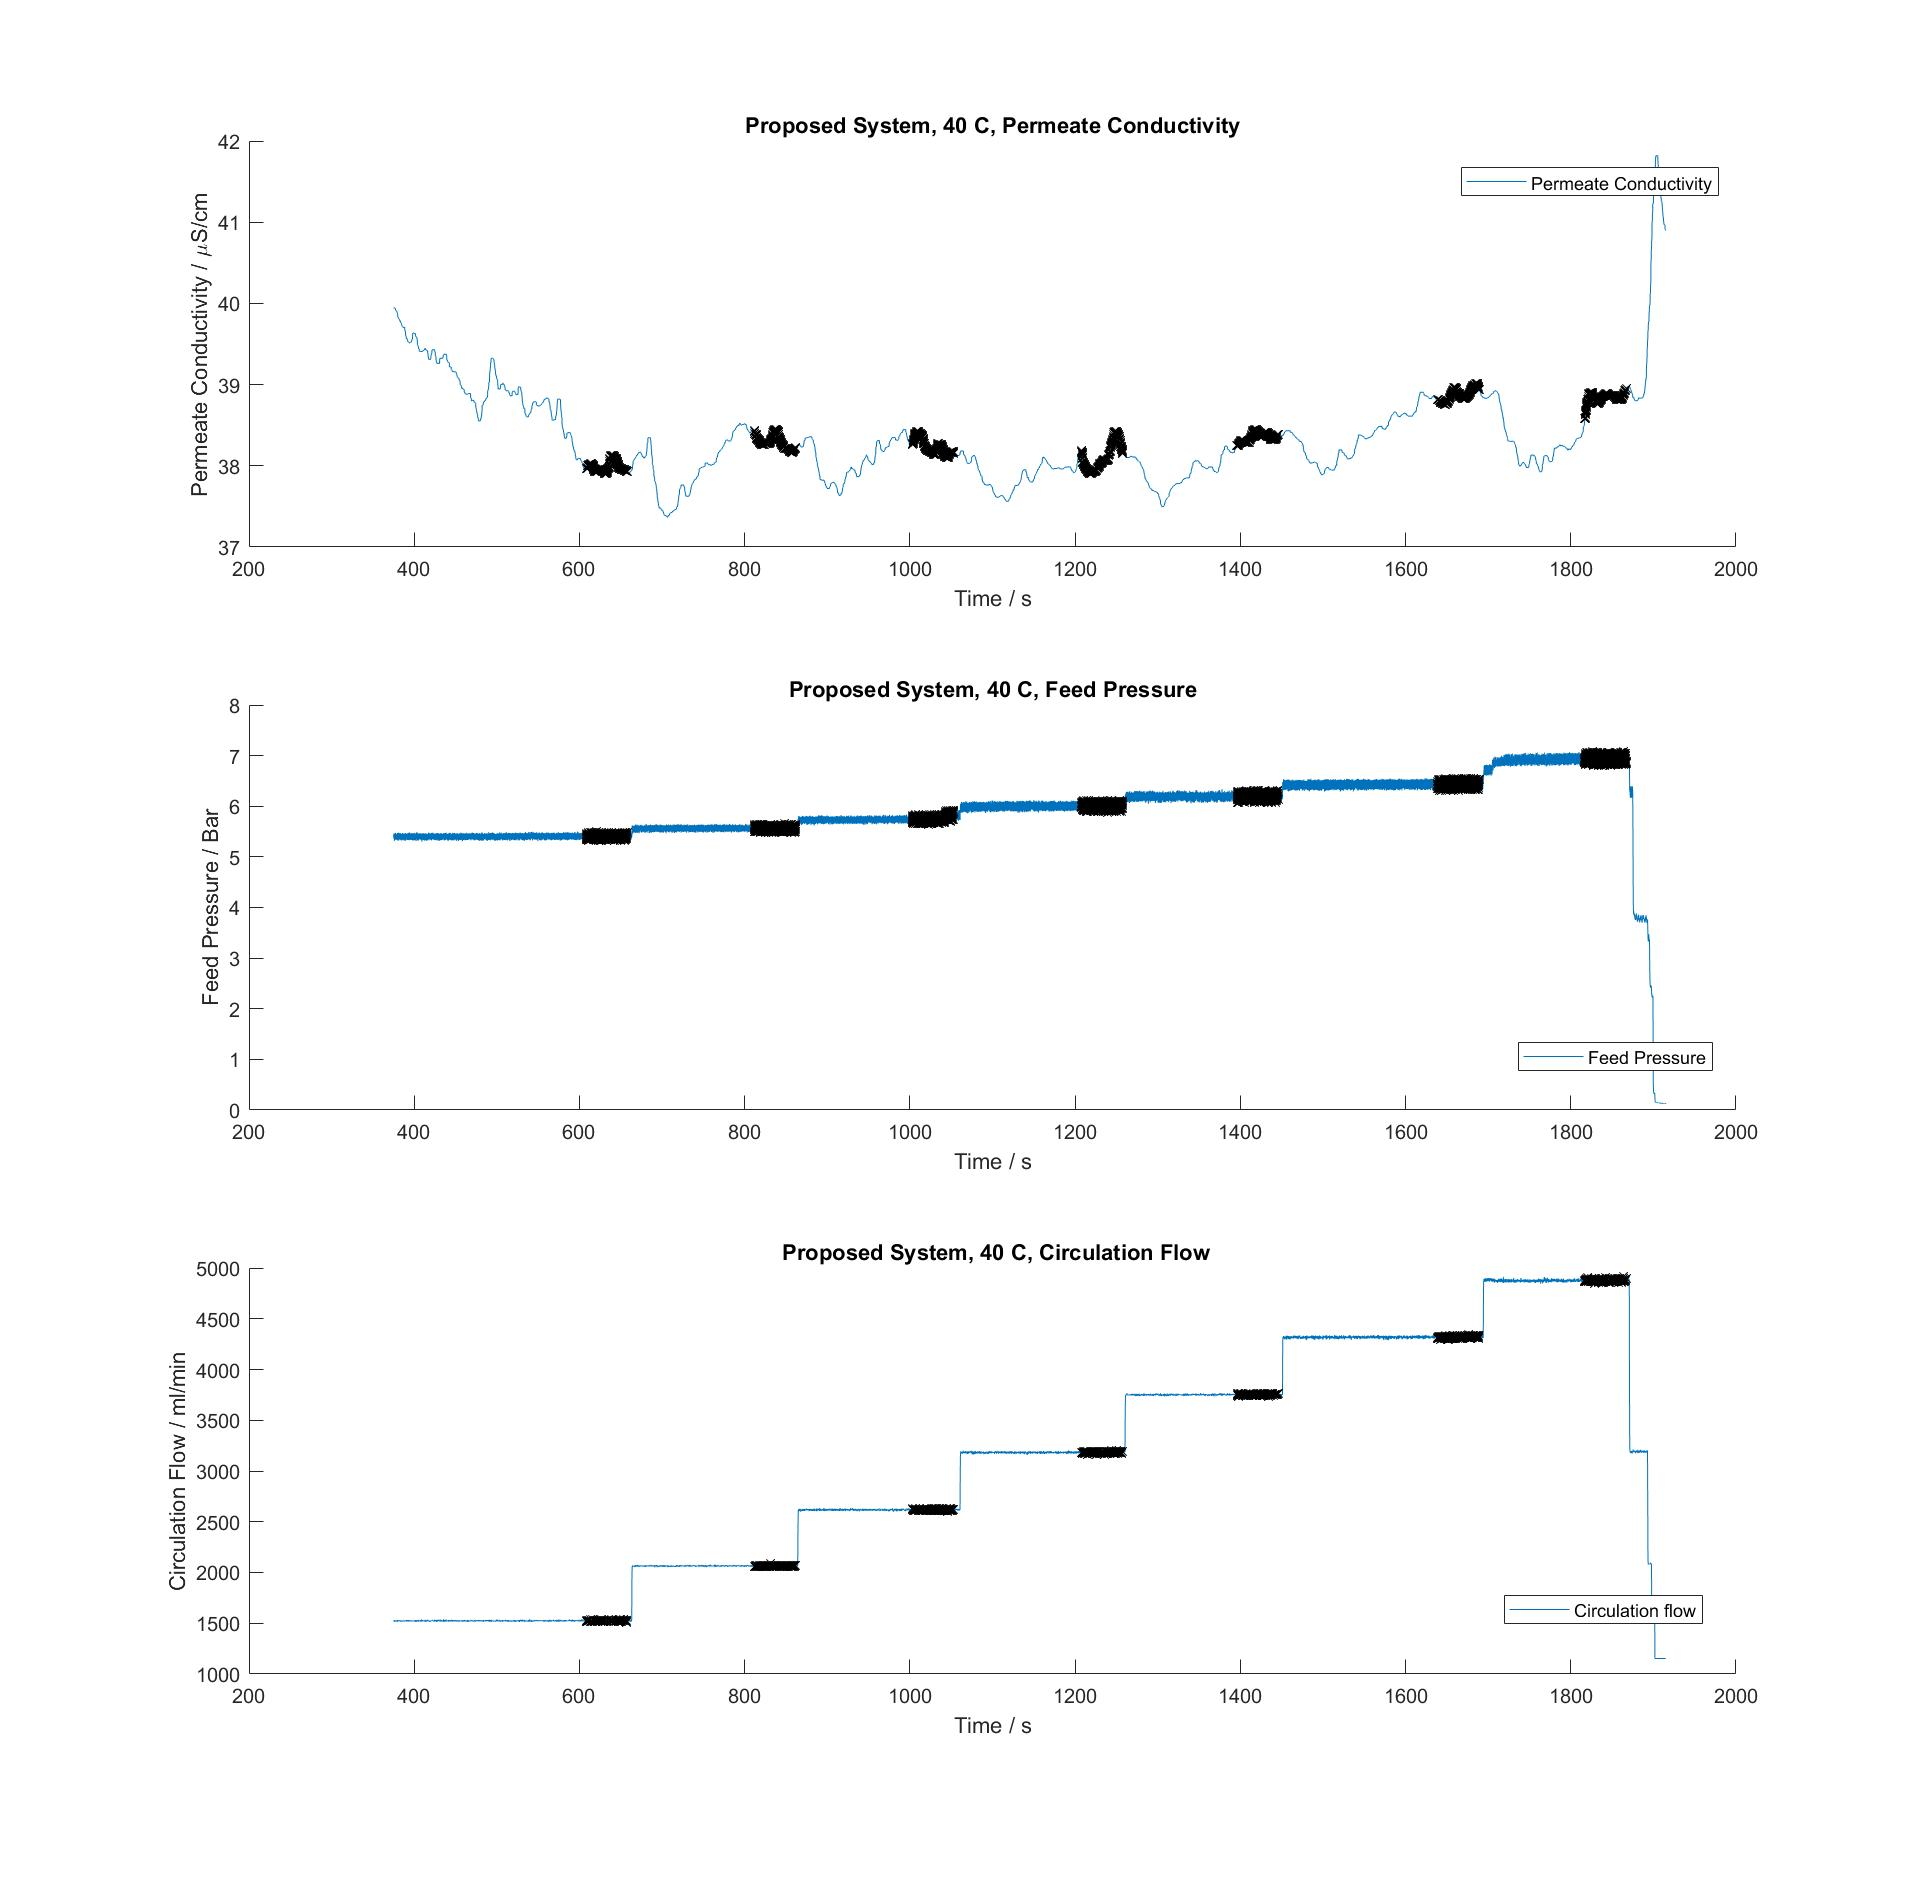
\includegraphics[width=1.1\textwidth]{RecIncrease40}
    \caption{Caption missing}
    \label{fig:RecIncrease}
\end{figure}  

More information about how the system performed during the test was calculated and can be seen in figure \ref{RecIncreaseKey}. The Recovery decreased from 22\% to 14\%  but salt rejection and permeate conductivity did only increase slightly. 
\begin{figure}[H]
    \centering
    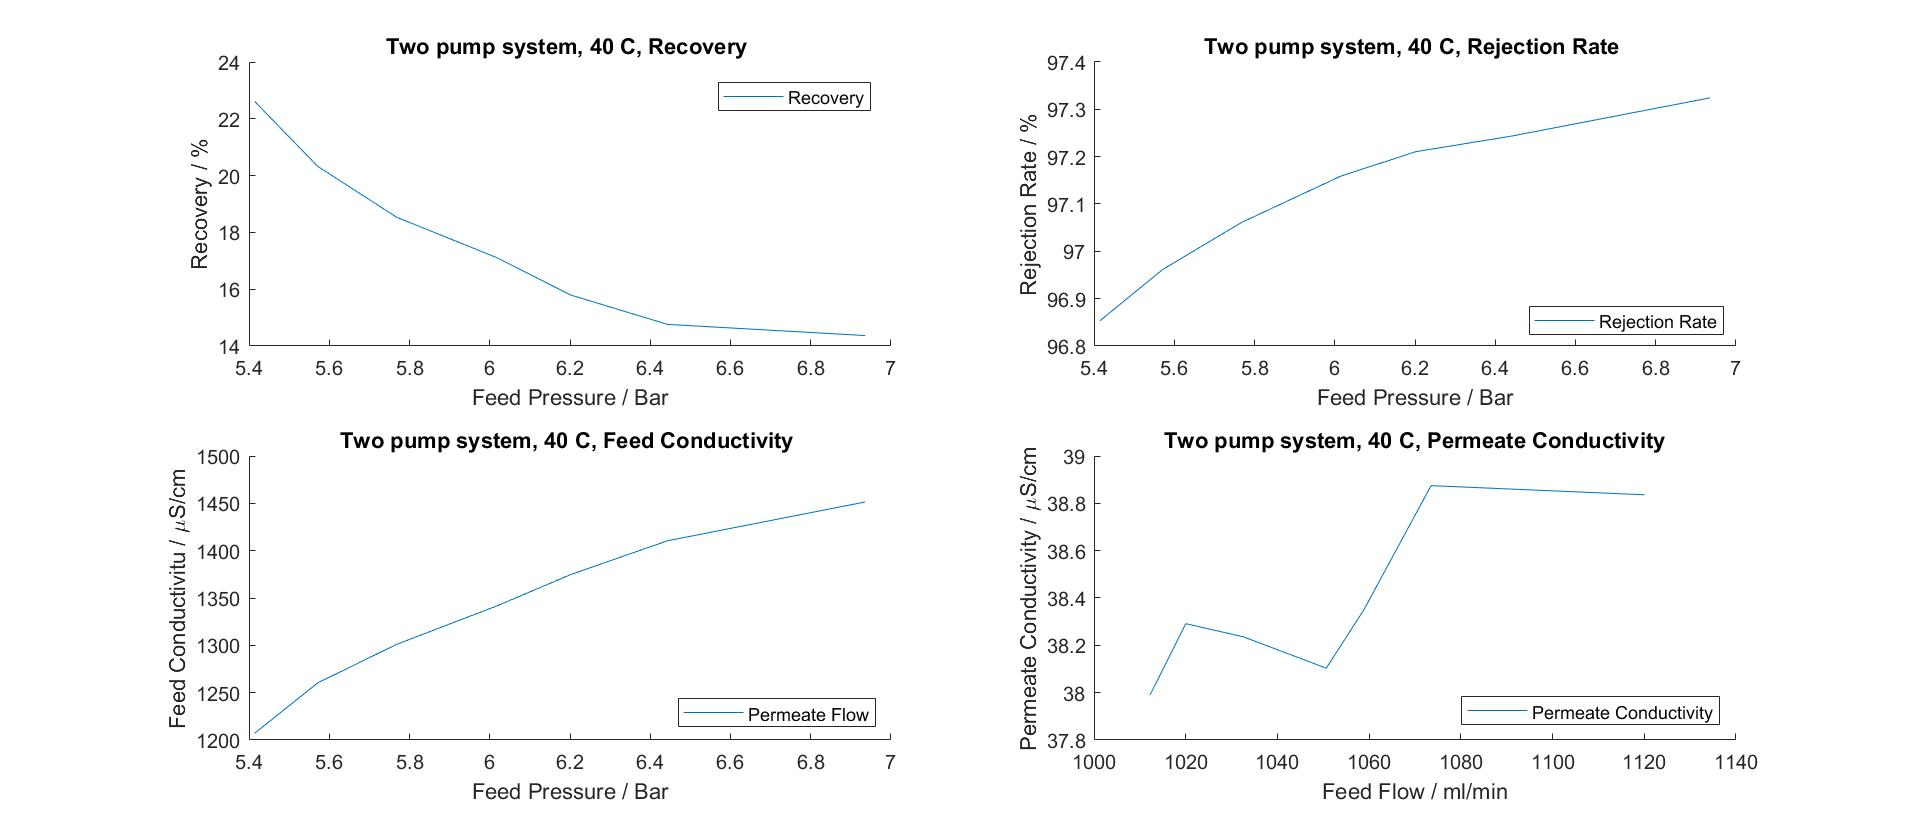
\includegraphics[width=1.1\textwidth]{RecIncrease40Key}
    \caption{Caption missing}
    \label{fig:RecIncreaseKey}
\end{figure} 
\par\bigskip 
\noindent
The test concluded that the initial theory that increased circulation flow would lead to better system performance was false. Increasing the circulation has no measureable positive effect on the system. 

\newpage
\subsubsection{increased circulation}
The next test was set up to investigate the effect of an increased feed pressure. During the test all parameters were kept constant except the rpm of the feed pump. An overview of the test can be seen in figure \ref{fig:FeedPumpIncrease40} and the key parameters calculated after the test can be seen in figure \ref{fig:FeedPumpIncrease40Key} 

\begin{figure}[H]
    \centering
    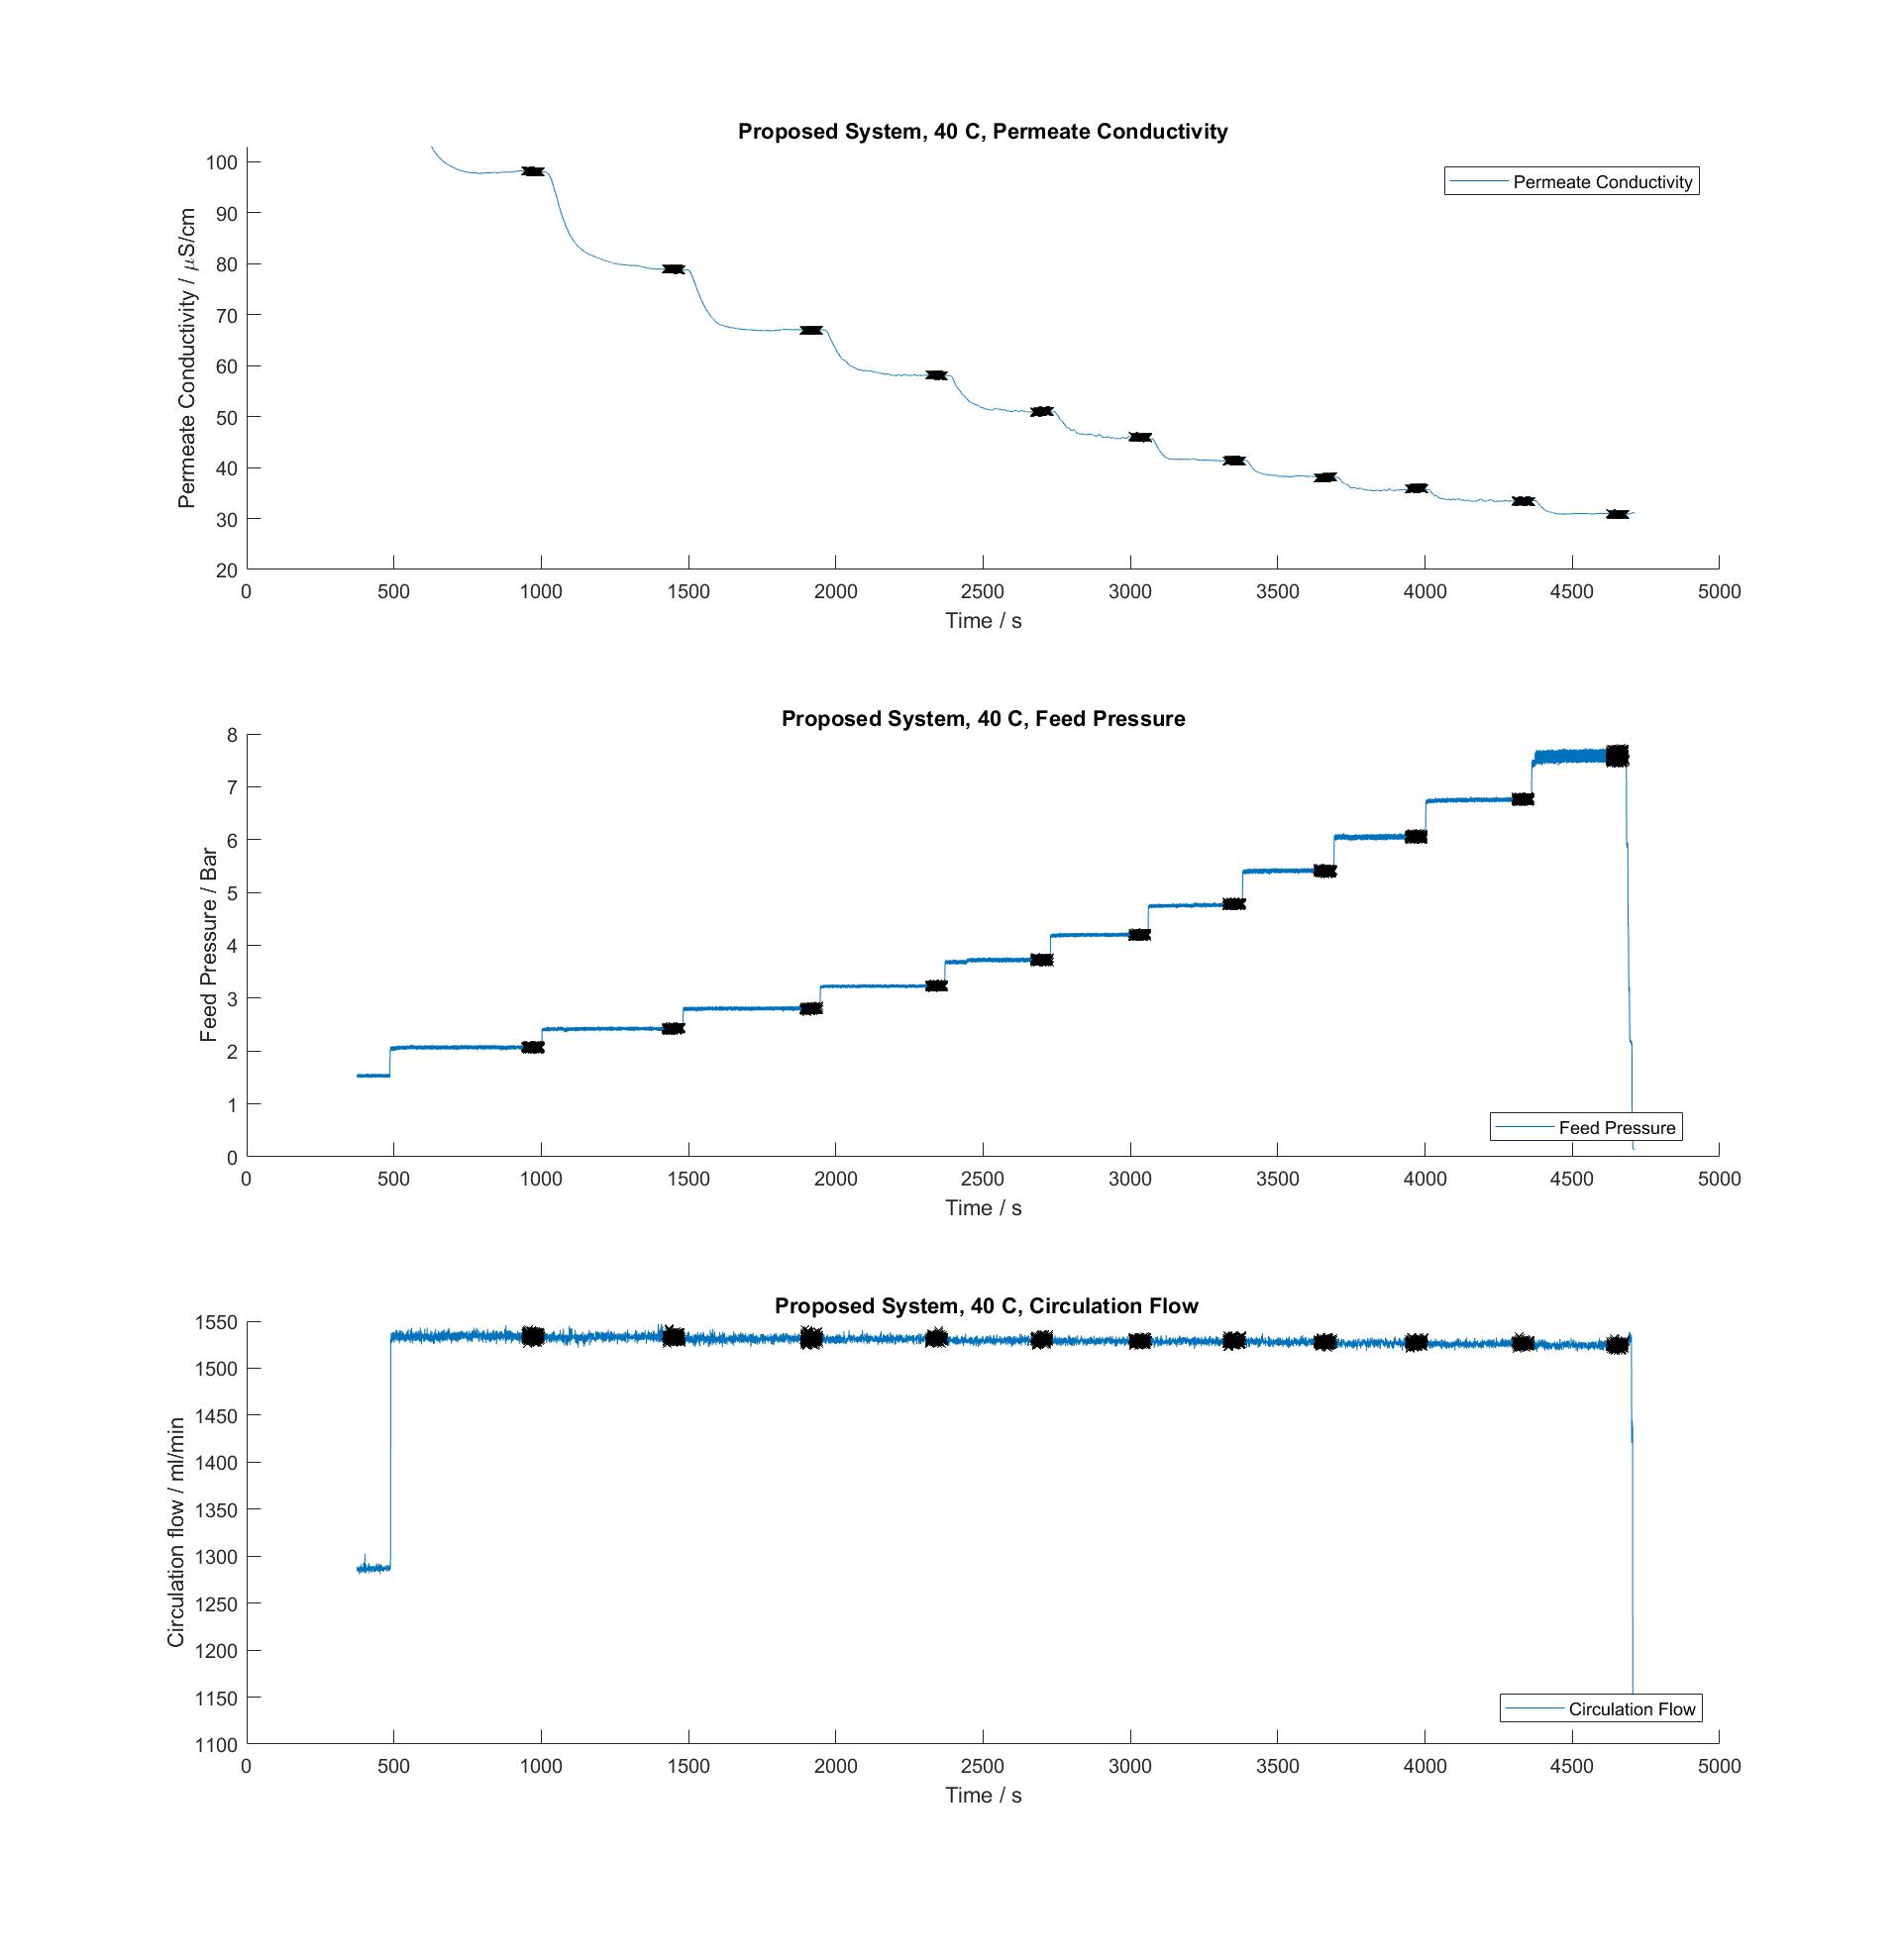
\includegraphics[width=1.1\textwidth]{FeedPumpIncrease40}
    \caption{Caption missing}
    \label{fig:FeedPumpIncrease40}
\end{figure}

\begin{figure}[H]
    \centering
    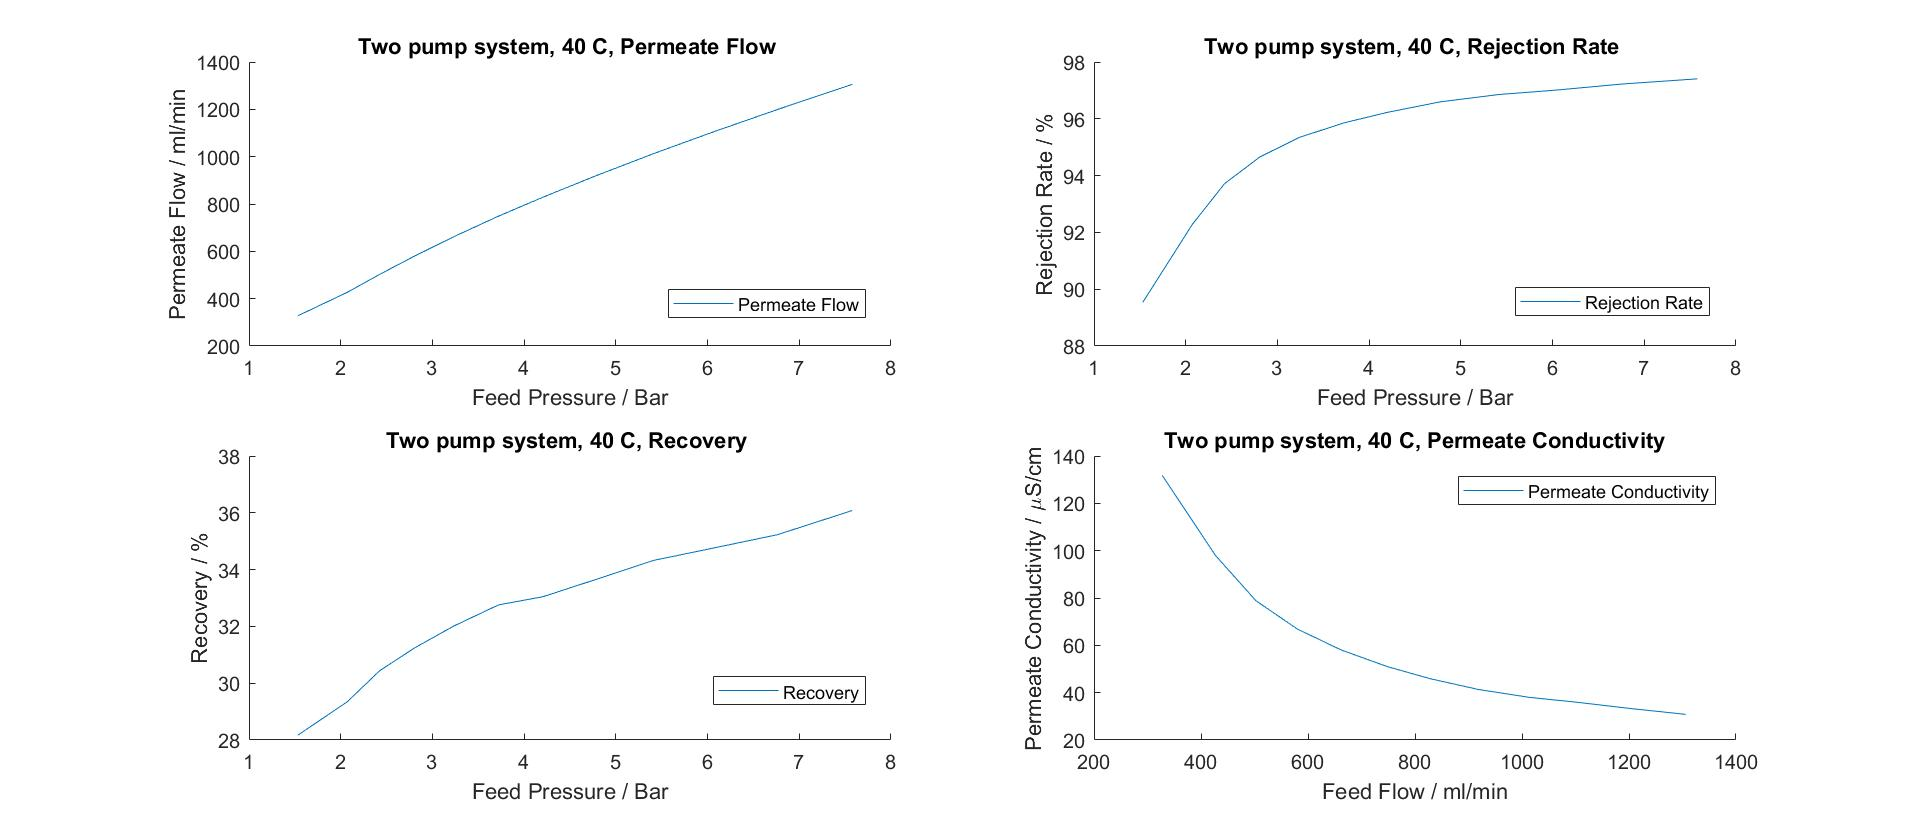
\includegraphics[width=1.1\textwidth]{FeedPumpIncrease40Key}
    \caption{Caption missing}
    \label{fig:FeedPumpIncrease40Key}
\end{figure}

From figure \ref{fig:FeedPumpIncrease40} it can be seen that the circulation flow remained constant and that the feed side pressure was increased from 1.5 to 8 bars. The permeate quality increased from 100 uS/cm to 30 uS/cm. As a result, it could be concluded that it was possbile to increase the performance of the membrane by increasing feed side pressure without the increased circulation flow. It should be noted that  the membrane recovery increased from 28\% to 36\% during the test and this is far above the maximum limit specified by the manufacturer. Therefore, it should also be concluded that only controlling the feed pump without controlling membrane recovery could damage the membrane. 

SAVING ENERGY COSTS WATER / VICE VERSA!


 
\newpage
\subsection{Optimization algorithm}

Previous tests concluded that it was ineffective to increase salt rejection by increasing the circulation flow, that it was possible to increase feed side pressure to increase salt rejection and that water temperature was the parameter that had the largest deterimental effect on salt rejection. Increased feed water conductivity also decreased the performance of the system, but not as much as increased temperature and the negative effect of high conductivity was more prominant at higher temperatures. Increased feed side pressure has a larger possitive effect on salt rejection at high temperature.
Since test showed that increased temperature decreased net driving pressure (See figure \ref{fig:NDP}) and that decreased feed pressure reduced salt rejection (see figure \ref{fig:SalrRejectionResult} it could be concluded that using a fixed value setpoint at either feed side pressure or permeate flow would not work. Instead a setpoint could be calculated for a given temperature and pressure or permeate flow could be used as a setpoint.
By using permeate flow instead of feed side pressure as a setpoint, factors such as membrane fouling, scaling and individual differences in the membrane could be compensated by the controller.

\subsection{Finding an optimal plane}

the purpose was to find a permeate flow setpoint that would ensure good quality peremeate at all temperatures without wasting more water and energy than needed. Since it was concluded in previous tests that membrane recovery did not improve saltrejection it was determined that this parameter should be set to 20\%. 

The goal of the test was to find the lowest pressure needed at a given feed conductivity and temperature to achieve a permeate conductivity of 30 uS/cm while maintaining a recovery of at most 20\%. The test was conducted by first adjusting the temperature in the heating bath to 20 deg C and then add salt so that the conductivity of the water in the bath was roughly 275 uS/cm. Afterwards, the feed and circulation pump were adjusted to obtain a  permeate conductivity of 30 uS/cm and 20\% recovery. Once the system had stabilised important parameters were noted. Once the parameters had been obtained, the conductivity was slowely increased and the pumps were modified to once again produce peremate water with a conductivity of 30 uS/cm. This procedure was repeated until the conductivity reached 3000 uS/cm. The same procedure was repeated using 30 C and 40 C inlet water.








 
 



 













\section{Mapping}
The mapping of the pumps RPM and flowrate can be seen in \ref{fig:RPM} and \ref{fig:Flowrate}.
\begin{figure}[h]
    \centering
    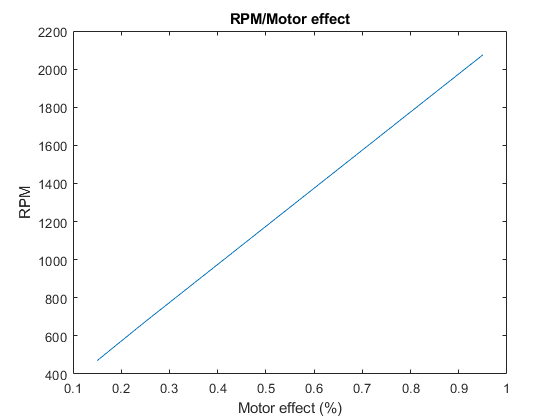
\includegraphics[width=0.7\textwidth]{RPM.png}
    \caption{RPM of the Pumps at different control signals/duty cycles}
    \label{fig:RPM}
\end{figure}


\begin{figure}[h]
    \centering
    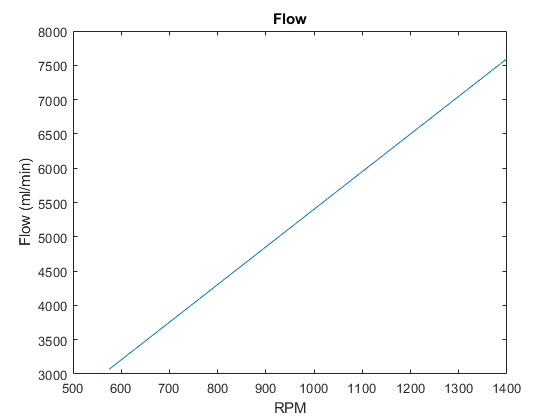
\includegraphics[width=0.7\textwidth]{Flow.png}
    \caption{Flow rate at different control signals/duty cycles}
    \label{fig:Flowrate}
\end{figure}


\section{Design of control algorithms}
In order to design control for driving the system some investigations on System 2, the two pump solution were done. In picture \ref{fig:PreTestReg1}, the results from test with all parameters except the speed of the recycle pump were kept constant, can be seen. \\
\\
In picture \ref{fig:PreTestReg3}, the results from test with all parameters except the speed of the feed pump were kept constant, can be seen.

\begin{figure}[h]
    \centering
    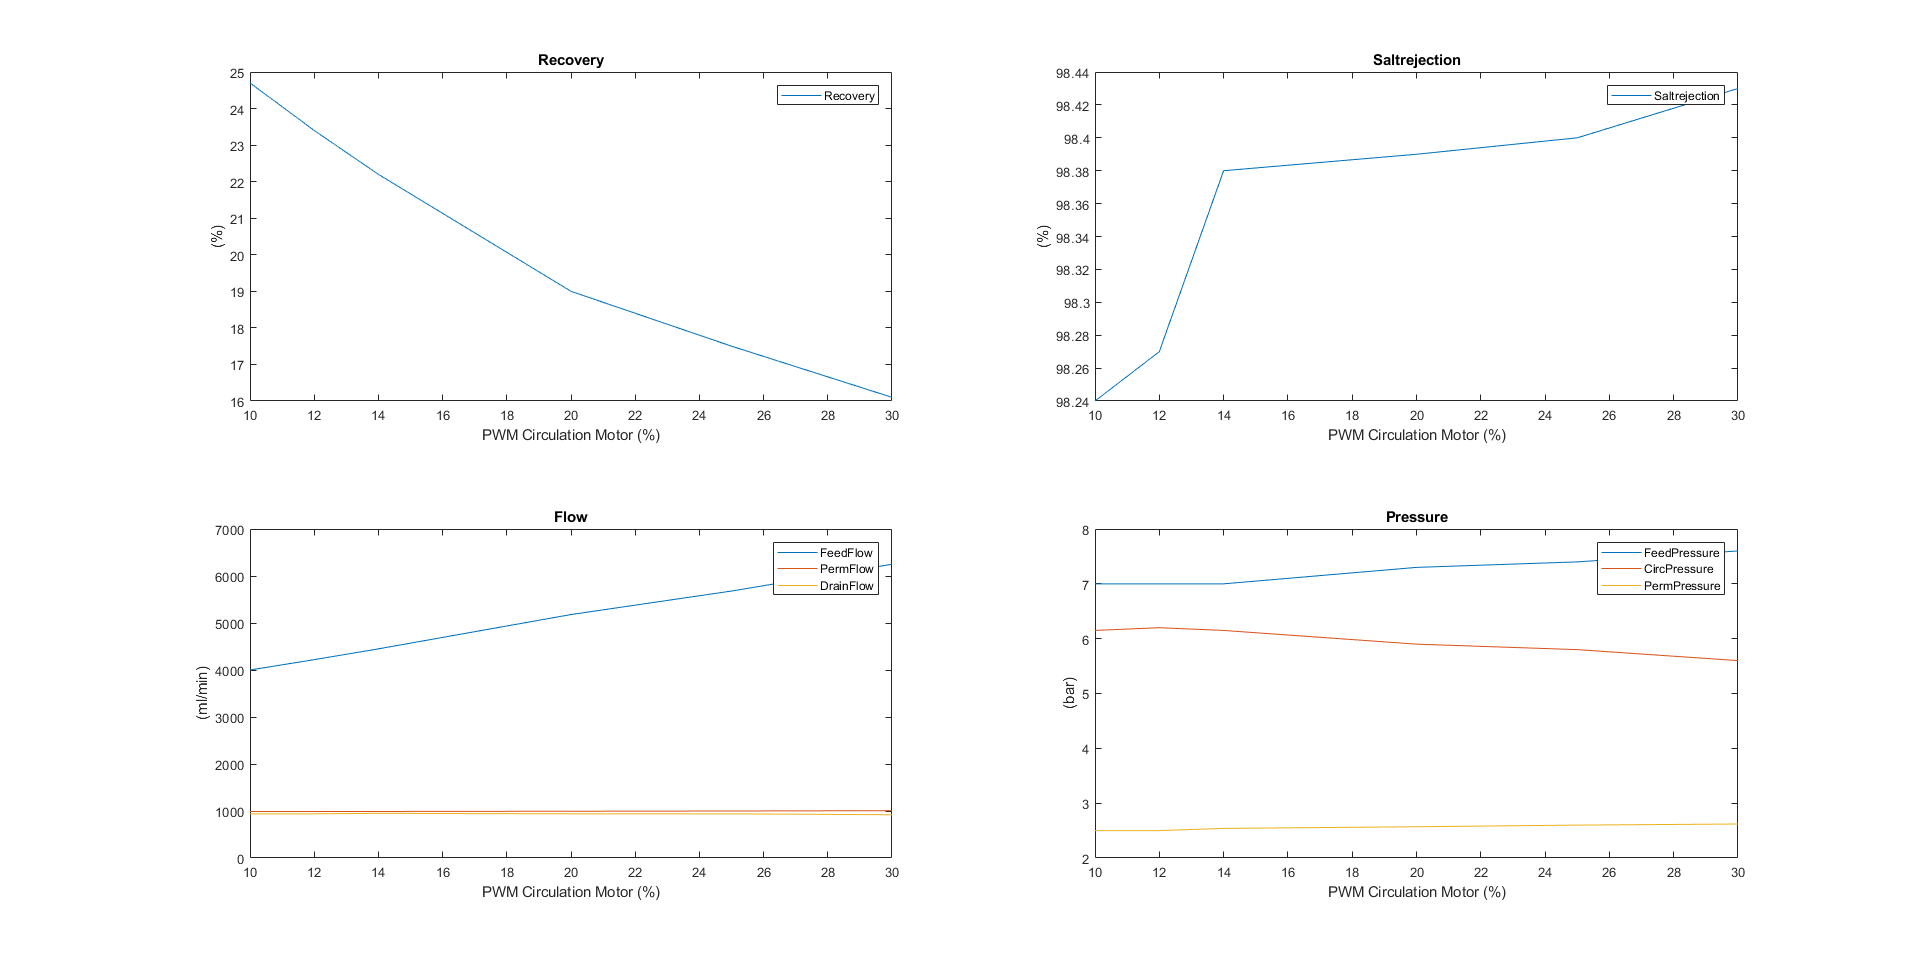
\includegraphics[width=1.65\textwidth, angle = 270]{PreTestReg1.png}
    \caption{Tests with recycle pump as changing parameter}
    \label{fig:PreTestReg1}
\end{figure}

\begin{figure}[h]
    \centering 
    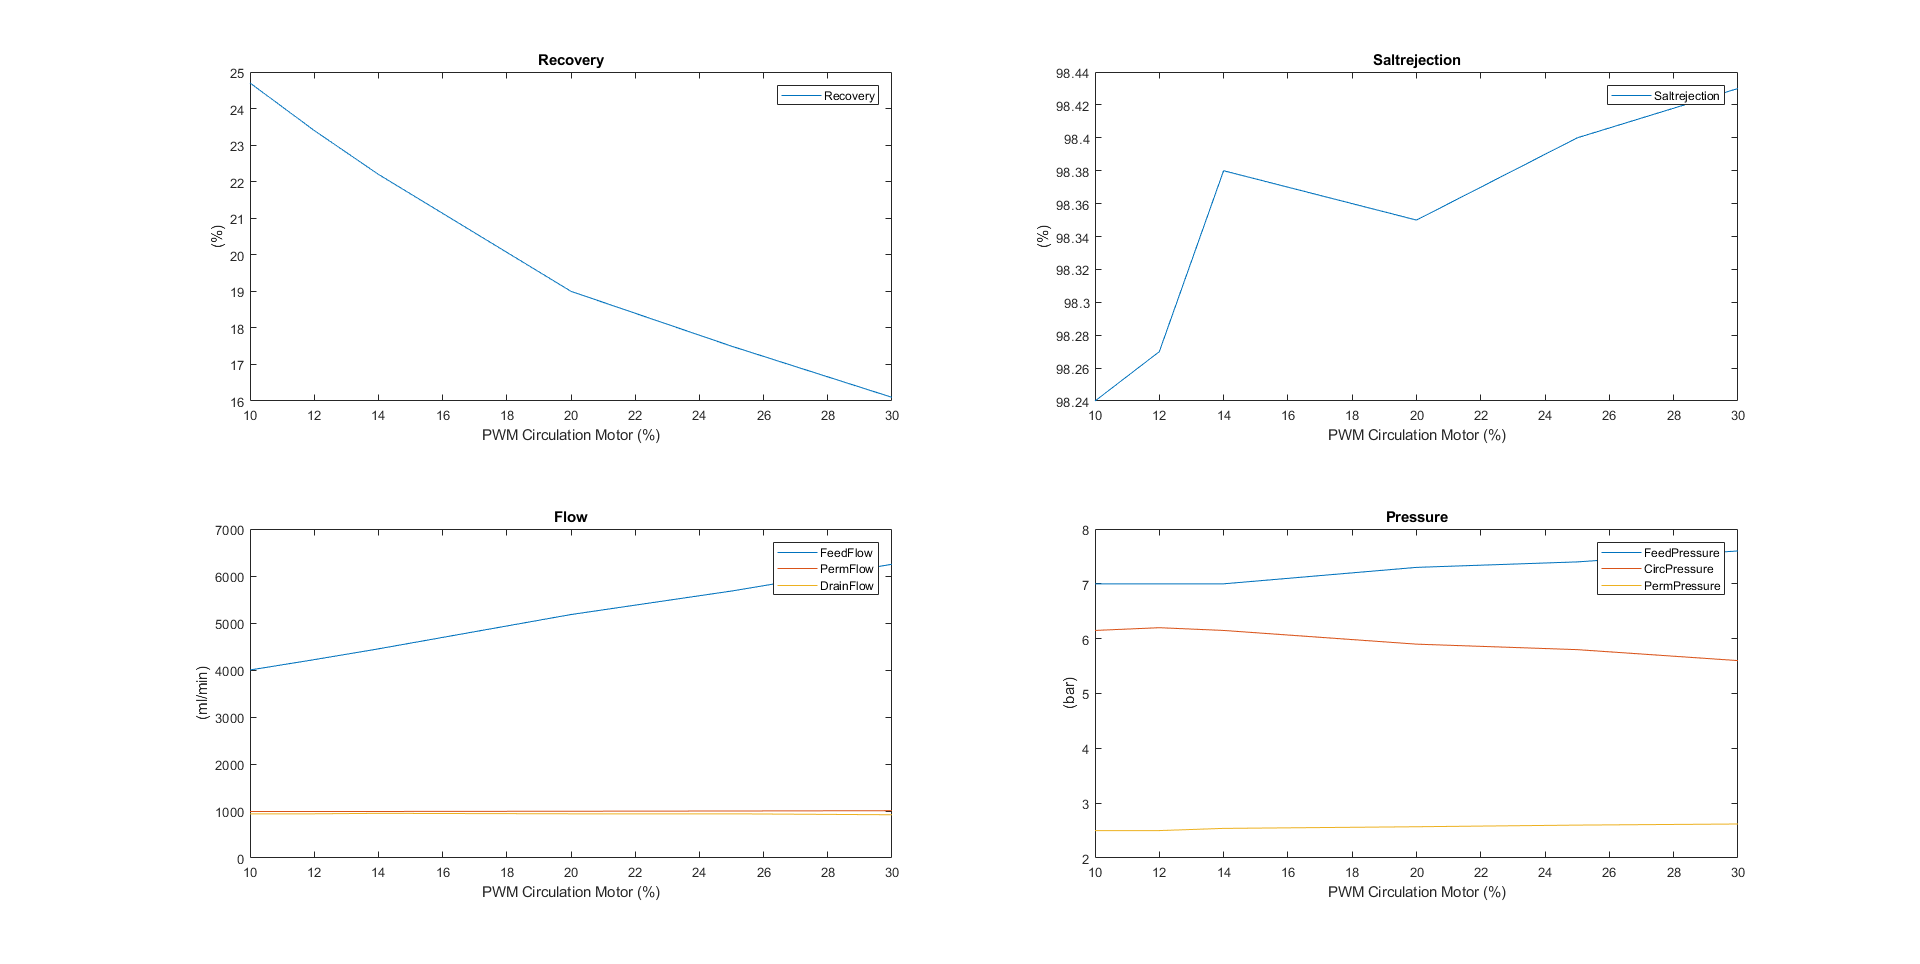
\includegraphics[width=1.65\textwidth, angle=270]{PreTestReg3.png}
    \caption{Tests with feed pump as changing parameter}
    \label{fig:PreTestReg3}
\end{figure}







\chapter{Discussion}
% !TEX root = /Users/Gela/Desktop/Thesis_latex/thesis.tex
\section{Simulations}
When performing the simulations in Simscape the main objective was to isolate the characteristics of the membrane functionally. The temperature dependencies in flow and pressure were expected to be implemented in the model. In order to receive good results, equations from DOW, the manufacturer of the membrane, were used. The results from the simulations showed that the membrane behaviour meets the constraints from theory. One important parameter is the temperature correction factor, plotted in figure \ref{fig:tcf}. It is used to compensate for the differences in temperature for the membrane performance, both in flow, pressure and conductivity and give the model some realistic behaviour in different temperatures. \\
\\
The simulations in Simscape showed significant results on the membrane behaviour. The flow characteristics over the membrane, due to changes in temperature, meets the expectations from the theory. Pressure characteristics, seen in figure \ref{fig:deltap} is a bit high, which probably is due to the pump and pipes simulated in the model. \\
\\


\section{System behaviour} 

%The test setup was built to understand how the performance of the reverse osmosis changed while operating in different conditions and by analysis the logs from the tests it was possible to understand the complexity of this multiple input and output system. Testing was mostly carried out by fixing all parameters but one and then change this parameter and log how the system behaved, this proved to be difficult because some parameters, for instance recirculation flow and feed pressure were directly connected to each other. However, analysis of the log files from the tests it was possible to understand how different conditions and setups affected the behaviour of the system. 

The main purpose of this thesis was to investigate the advantages of using a two-pump system instead of the current one pump system. We found that there were multiple advantages of using the two-pump system, the overall power consumption and noise levels could be reduced without reducing permeate quality or water efficiency. The new setup also had the unforeseen advantage of reducing the pressure drop over the membrane, from feed to reject side. This was a result of changing the position of the inlet pump from inside of the recirculation loop to pumping straight into the loop and using the recirculation pump to create the desired flow. The reduced pressure drop causes the membrane to be more evenly pressurized, creating a more uniform permeate flux accross the membrane surface, this could in theory prevent the uneven scaling of the membrane.\\
\\
Initially, it was believed that a higher recirculation flow would improve the performance of the membrane by increasing the flow rate over the membrane surface and thereby causing a more turbulent flow that would mix high salinity water close to the membrane with less saline water further from the membrane. However, tests showed that this was not the case. The performance did improve by a small amount, but by increasing the recirculation flow, the pressure was also increased and the small improvements that could be observed was more likely caused by the increased pressure on feed side, not the increased flow rate from feed to reject side. Therefore, it was concluded that there was a no possibility of effectively optimize the membrane by increasing the recirculation flow. \\
\\
According to the membrane manufacturer the recovery rate should not exceed 20 \% in order to ensure the longevity of the membrane. It was decided to use the recirculation pump to ensure that the recovery remained fixed at 20\% and not use this parameter for optimization.\\
\\
Feed pressure has a direct effect on both permeate flow and salt rejection. The physical reason for the improved salt rejection is that a larger volume of water passes through the membrane surface and dilutes the dissolved salts that also passes. This can be seen in figure \ref{fig:FeedPumpIncrease40}, from this data it can also be concluded that salt rejection does not increase linearly with increased pressure and that the positive effect of an increased feed pressure is greater at low pressure, for instance an increase from 2 to 4 bar has a larger positive effect than an increase from 7 to 9 bar. As a result, improving the performance of the membrane has low cost at low pressures but becomes more and more expensive when the pressure increases.\\
\\
Hot water has lower viscosity than cold water and also a higher diffusion rate than cold water. The pores of the membrane are also expanding at higher temperatures, causing a higher flow through the membrane from feed to product side. Consequently, higher temperatures cause higher permeate flow over the membrane and increased salt passage through the membrane surface. If both water and salt passage were equaly affected by temperature the rejection rate would not change with changing temperature but high temperatures makes it easier for salts to pass through the membrane surface than water, resulting in a larger flow of water that contains a proportionally larger amount of dissolved salts. In order to improve the salt rejection rate more permeate needs to pass through the surface to dilute the salts and this can be achieved by increasing feed side pressure, causing a higher flow. \\
\\
The conductivity of the inlet water is also a quantity that depends on the tap water and determines the lowest possible conductivity of the recirculation loop. By using permeate conductivity as a set point for controlling the drain valve it is possible to optimize the water efficiency of the system and ensure high quality permeate water. Lower conductivity feed water allows the system to recirculate more water without reaching the critical limit where a permeate conductivity of 30  can not be maintained. Therefore, the system can adapt to different feed water conductivity by adjusting the drain valve.\\
\\
Net driving pressure depends on the feed pressure in the recirculation loop, permeate side pressure and also the osmotic pressure caused by the different salt concentrations across the membrane. In order to save energy, it is beneficial to have a low permeate side pressure and lower conductivity in the recirculation loop. In order to save water, the control loop controlling the drain valve accumulate high conductivity water in the recirculation loop which increases NDP, net driving pressure. However, this drawback is necessary to maintain a high water efficiency and in the authors opinion, the slight decrease in NDP is worth the increase in efficiency. It is possible to increase the feed side pressure by increasing the pump speed, although, this requires more energy. The only way to improve the NDP of a system without decreasing water efficiency or increasing energy is to decrease the permeate side pressure. This can be done by selecting components on permeate side with a low pressure drop and by using a short flow path.

\section{One vs two pump system}

In the one pump system, the feed pump creates both flow and pressure and these parameter are therefore coupled to each other and cannot be changed independently. The pressure is generated by the resistance in the membrane and also in the recirculation restrictor. As a result, the feed pump must deliver a large amount of water to build the pressure needed to push the water through the membrane surface. \\
\\
By changing the flow path and adding another pump the feed pump can pressurize the circulation loop without a high water flow. As a result, the feed pump can run at a much lower rpm. The circulation pump creates the flow but does not have to generate any pressure since the circulation loop is pressurized by the feedpump.

\section{Fine tuning}

The PID parameters for the controllers could be changed at runtime in the simulink real time GUI and the PID parameters that were used was found by trial and error. We found that the recirculation, and permeate flow controller could be fast without causing problems. The drain valve controller on the other hand needed to be very slow to not cause oscillations. \\
\\
No effort was made to try to find the best possbile PID parameters for the control loops. Since the pumps or the drain valve most likely would be changed if there were any further development on the two pump system we choose not to spend time trying to make the system as fast and stable as possible and instead focus on the algorithm. \\
\\
\section{Control System Design}

There were two main properties that was to be optimized, water efficiency and energy consumption. The conductivity of the permeate water should also be controlled.\\
\\
A PI controller was used to control the conductivity of the permeate by opening or closing the drain valve. Salt rejection changes with different temperatures and feed pressure, because of this, the recirculation loop can only hold a certain amount of dissolved salts in order to maintain a permeate of 30 \SI{}{\micro\siemens}/cm. For instance, if the system has a salt rejection of 99\% the recirculation loop must hold water with a conductivity of 3000 \SI{}{\micro\siemens}/cm to obtain a 30 \SI{}{\micro\siemens}/cm permeate. If the system saltrejection change to 96\% then the conductivity in the recirculation loop must be 750 \SI{}{\micro\siemens}/cm to achieve the same permeate quality. As can be seen in figure \ref{fig:Permeatecond} from the tests with the current system, a system with room temperatured inlet water was able to maintain 30 \SI{}{\micro\siemens}/cm permeate water with 2500 \SI{}{\micro\siemens}/cm in the recirculation loop but if the inlet water was heated to 40 degrees Celsius only 1500 \SI{}{\micro\siemens}/cm recirculation conductivity was needed to reach 30 \SI{}{\micro\siemens}/cm. Thereby, controlling the valve position was critical to being able to make sure that the permeate conductivity was 30 \SI{}{\micro\siemens}/cm regardless of operating conditions. \\
\\
Opening the drain valve lowers the conductivity in the recirculation loop but it takes time to reach a new steady state. This caused a problem because if the changes were not slow the system would overshoot. The only way to fix this problem was to use a slower controller.\\
\\
%Since the recirculation loop and the membrane contains about TBD liters of water the response from changing the drain valve was slow, much longer than the other control loops which has an almost immediate effect. Because of this it was necessary for the controller to slow. 
An increase in pressure resulted in more fluid getting pushed out of the drain valve without the position of the valve being changed. As a result, changes in pressure will act as a disturbance on this control loop. To counter the effect of this, the valve needs to close to make sure that no water is unnecessarily being rejected to drain. However, closing the valve will result in an increased pressure in the system that needs to be handled by the controller controlling the pressure in the system. This means that these two controllers are coupled to each other and that it is impossible to change one without influencing the other. Because pressure can be changed quickly, this problem could be fixed by using a much faster controller for the controller controlling the feed pressure pump than the drain valve.\\
\\
Tests showed that increased recovery did not affect the salt rejection of the system. For this reason, it was decided to set the recovery setpoint to approximately 20 \% which was the recommended recovery from the membrane manufacturer. This regulator had little impact on the regulator controlling the drain valve but when the flow in the recirculation loop increase so does the pressure in the loop. The effect of this can be seen in figure \ref{fig:RecIncrease40}. From the plots it can be seen that 22 \% recovery caused a pressure of 5.5 bars and a recovery of 14 \% increased the pressure to 7 bars. Therefore, the regulator pressurizing the recirculation loop act as a disturbance on the recovery regulator.\\
\\
The last controller was the controller tasked with optimizing the membrane. Warmer inlet temperature increases the amount of salts that pass through the membrane as well as the water. However, the increased temperature increases the salt passage more than the passage of water, resulting in a higher permeate flow with a higher conductivity. The only way to counter this phenomenon and increase salt rejection is to increase the permeate flow by increasing feed pressure and dilute the increased salt in the increased permeate flow. By using the formula to convert feed water temperature to a set point for the permeate flow the salt rejection of the membrane could be optimized. This design allows the system to counter the detrimental effect that increased temperature has on the salt rejection of the membrane at the cost of using more energy. The increased salt rejection allows higher conductivity water to be accumulated into the recirculation loop and thereby water efficiency is increased. In figure \ref{fig:SaltRejectionResult} it can be seen that increasing feed pressure has a larger positive effect on salt rejection when the inlet temperature was high and therefor there is no need to waste energy running the system at high pressure. In this scenario, it is better to save energy by running the system at lower pressure and permeate flow. \\
\\
The system was designed to be able to deliver a stream of permeate water with a conductivity of 30 \SI{}{\micro\siemens}/cm without using more energy and rejected water than necessary, but our tests showed that the only way to increase salt rejection and lower the amount of rejected water was to increase the permeate flow. This means that there is a trade-off between water efficiency and energy efficiency. Running the system on low pressure decreases salt rejection and thereby less salts can be recirculated back into the recirculation loop and this means that more water is wasted. By testing, the lowest permeate flow that generated a permeate conductivity of 30 \SI{}{\micro\siemens}/cm at different temperatures could be found and these results were translated into a function for what permeate flow should be used as a set point at different temperatures. 

\section{Noise reduction}

An additional positive effect of using two pumps instead of one was that there was a significant reduction in noise. Since this effect was not a part of the initial scope and just a positive side effect of using two pumps no data was gathered to support the claim, but the difference could be heard when both systems were tested. The reason for the noise reduction was that both the two pumps were running at much lower rpms when using two pumps. 

\section{Reduced pump size}
When using the two pump system the pump speeds varied from 3\% to 25\% depending on the permeate flow setpoint which is a reduction from the 60 \% and 80 \% used when one pump was used. This indicate that it might be possible to use smaller pumps. Smaller pumps could allow the system to be smaller and they are often cheaper than larger pumps. This reduction of the prize could reduce the increased cost of buying two pumps instead of one. Smaller pumps might also be more quiet.

\section{Membrane size}
Membrane size determines the permeate flux at a certain pressure and for smaller systems it might be beneficial to reduce the size of the membrane to make the device smaller and possibly cheaper. In addition to the reduced size and prize a smaller membrane has less pressure drop and more even pressure over the whole membrane.

\section{Membrane identification method}
This report is based on the DOW FilmTec membrane used by Baxter today and the temperature to optimal permeate flow function will only work for this membrane. However, the method for finding this function can be used on any membrane. By following the method outlined in this report this function can be found for any other reverse osmosis membrane and can be modified for other specifications on permeate quality. 

\section{Scaling}
One advantage of using a permeate flow set point for the feed pump controller is that it will let the system adapt to scaling. When scaling occur, the membrane surface becomes coated with suspended solids that clogs the surface of the membrane. Using the control design from this thesis, when the membrane surface clogs up more pressure is needed to reach the permeate flow setpoint and this will automatically be achieved by increasing the feed pump. Membrane fouling is inevitable and eventually the membrane will have to be replaced. Even though membrane fouling can't be stopped it can be minimized by following the operational guidelines from the membrane manufacturer. One of these guidelines is the maximum allowed recovery and by controlling this parameter with a control loop, the system improves the longevity of the membrane. 

\section{Drain valve}
The valve used in the test rig was built for much larger systems and is not intended for fine tuning. This caused problems because it was not possible to make small changes and this caused oscillations in the conductivity of the permeate. Because it was clear what caused the oscillation and that it would take a lot of time to find, order and rebuilt the test rig with a new valve we choose to continue using the valve. If there are any further development of the system, the valve should be replaced.\\
\\

\chapter{Conclusion}
% !TEX root = /Users/Gela/Desktop/Thesis_latex/thesis.tex
The permeate quality of an RO-system is reduced considerably when the system is running on hot water due to the decreased salt rejection. The results from our tests showed that the most effective way of incresing permeate quality was to create a higher permeate flow when the system was hot to dilute the increased salts in the permeate with a larger volume of water. By identifiying what permeate flows are needed at different temperatures it is possible to find an optimized permeate flow for every temperature within the operating range.\\
 \\
By replacing the current one pump system without any feedback loops with a system using two pumps and PI regulators and the ability to control the system allow a more optimzed performance on both water efficiency and energy consumption. As mentioned, the current system does not use any feedback controllers and therefore it cannot adapt to the changing behaviour that is introduced by changing temperatures. The modified system however, can measure and adapt to changing working condition and improve the performance of the membrane. \\
 \\
Since the performance of the membrane improves when it is subjected to more feed side pressure it can be argued that the system can be optimized by always applying maximum feed pressure. However, generating pressure costs energy and at low temperatures this extra energy might not be worth the cost even if it improves water efficiency by increasing salt rejection. Consequently, running the system at low pressure will cost less energy but waste more water. Therefore, it is not possible to optimize energy consumption without reducing the water efficiency of the system and vice versa. As a result, to optimize the system it needs to be determined which one of these parameters is considered to have the highest cost. \\
 \\
The model of the reverse osmosis membrane is build around the theoretical equations presented by DOW. These equations are accurate in describing the flow and pressure characteristics at different temperature. However, DOW is using a fixed rejection rate for all temperatures and does not incorporate the diluting effect that occurs when pressure is increased.  To be able to make a more accurate model this phenomenon needs to be matematically described and added to the model. \\
 \\
 The two pump system that is proposed in this thesis is more energy efficient in all working condition than the old one pump system. By looking at figure \ref{fig:EnergySys2} it is clear that the gains are substantial. \\
  \\
To summarize, the feedback controlled two pump system is a viable solution with several benefits over the current system and it is possible to optimize water efficiency and power consumption when using two pumps that would not have been possible with one pump. 

\chapter{Future Prospects}
% !TEX root = /Users/Gela/Desktop/Thesis_latex/thesis.tex

\section{Parameters of concern}
Saltrejection
Recovery


\section{Optimization}

Energy efficiency
Water efficiency



\section{Mapping}
This work is a first step in investigating the possibility to optimize the performance of the membrane. It can be seen that there are great possibilities, but in order to achieve an optimum performance more mapping is to be done. The main factors that is seen and a proposal for further investigations are:

\begin{itemize}
\item XXX
\item XXX
\end{itemize}


\section{Membrane size}
As seen in the tests the permeate water quality is due to the flow and salt rejection rate. In order to design devices that will deliver as clean and purified water as possible it might be beneficial to use smaller membranes when lower permeate flow is needed. Today there are recirculation paths from permeate side back to tank where clean purified water is mixed with inlet water, which might not be neccssary if down scaling the membrane.










\printbibliography 
\clearpage
\appendix
\chapter{Appendix A} 
\label{A}
%\input{}



\end{document}


